\documentclass[twocolumn,10pt]{article}
\usepackage[margin=0.68in,top=0.72in,bottom=0.74in,columnsep=0.24in]{geometry}
\usepackage{amsmath,amssymb}
\usepackage{booktabs}
\usepackage{array}
\usepackage{graphicx}
\usepackage{xcolor}
\usepackage{caption}
\usepackage{fancyhdr}
\usepackage{hyperref}

\setlength{\emergencystretch}{1.6em}
\renewcommand{\topfraction}{0.92}
\renewcommand{\bottomfraction}{0.86}
\renewcommand{\textfraction}{0.08}
\renewcommand{\floatpagefraction}{0.86}
\raggedbottom

\definecolor{linkblue}{HTML}{124E78}
\captionsetup{font=small,labelfont=bf,skip=4pt}

\hypersetup{
  colorlinks=true,
  linkcolor=linkblue,
  citecolor=linkblue,
  urlcolor=linkblue,
  pdftitle={A 62.58-Octave, 1,083-Star Prospectively Locked Panchromatic and Multi-Messenger Search for Extraterrestrial Technosignatures (SETIsearch D079-D112)},
  pdfauthor={Martin Andersen}
}

\pagestyle{fancy}
\fancyhf{}
\fancyhead[L]{\footnotesize\textcolor{gray}{Andersen (2026) --- Panchromatic \& Multi-Messenger SETI Synthesis (1,083 Targets, 62.582 Octaves, D079--D112)}}
\fancyhead[R]{\footnotesize\textcolor{gray}{\thepage}}
\renewcommand{\headrulewidth}{0.3pt}
\setlength{\headheight}{13pt}

\title{\vspace{-0.8em}\textbf{\Large A 62.58-Octave, 1,083-Star Prospectively Locked Panchromatic and Multi-Messenger Search for Extraterrestrial Technosignatures}}
\author{\textbf{Martin Andersen}\\[0.25em]
\small University of Copenhagen · \href{https://github.com/andersenmartin-blip/setisearch}{https://github.com/andersenmartin-blip/setisearch}}
\date{\small 26 November 2026 · Survey Phases \texttt{D079--D112} (\texttt{V7.0})}

\begin{document}

\twocolumn[{
\begin{@twocolumnfalse}
\maketitle
\vspace{-0.9em}
\begin{abstract}
\noindent Searches for extraterrestrial technosignatures have historically operated within narrow wavelength windows---typically $\lesssim 1.4$ octaves at $1.4\,\mathrm{GHz}$ radio or in visible optical echelle bands---leaving vast regions of the electromagnetic spectrum, polarization state space, and non-electromagnetic messengers weakly constrained. Here we synthesize thirty-four prospectively locked archival survey phases (\texttt{D079--D112}, software releases \texttt{V3.0--V7.0}) uniting \textbf{72 spectrographs, high-energy observatories, and interferometric/neutrino arrays (104 spectral arms)} across \textbf{62.582 electromagnetic (EM) octaves} ($1.239842\times 10^{-15}\text{--}8{,}556.41831\,\mu\text{m}$) plus $0.1\,\mathrm{TeV}\text{--}10\,\mathrm{PeV}$ \textit{IceCube} point-source muon neutrinos ($\nu_\mu$), $2.0\text{--}8.0\,\mathrm{keV}$ \textit{IXPE} X-ray linear polarimetry, and $0.37\text{--}2.515\,\mu\text{m}$ dual-beam optical/NIR Stokes $(I,Q,U,V)+N_1,N_2$ spectropolarimetry. Every phase sealed cryptographic algorithm, target, and veto definitions (\texttt{METHOD\_LOCK.json}) prior to science download against all prior observation IDs and coordinates, calibrated empirically across \textbf{113,967 synthetic injection-recovery trials} (all 43 suites passing $\ge 97.5\%$, reaching $9{,}072/9{,}111 = 99.57\%$ in \texttt{D112}), and verified bit-for-bit across \textbf{38 Companion Archives \texttt{A--AL}} ($657.49\,\mathrm{MiB}$) using pure-stdlib \texttt{/usr/bin/python3 -S} audits.\par\smallskip
\noindent Across \textbf{1,083 unique targets} ($787$ Science [$327$ exoplanet hosts with $576$ confirmed planets] $+ 296$ Control benchmarks), \textbf{4,383 archival exposures} (\textbf{736,410.27\,h}), \textbf{252 multi-epoch Keplerian orbital drift campaigns} (achieving \textbf{100.0\%} \texttt{DRIFT\_V67} closure across all $61/61$ known exoplanet hosts within $10\,\mathrm{pc}$), \textbf{753 all-sky frequency-comb stacks}, \textbf{10/10 \textit{ALMA} receiver bands (\texttt{B1, B2, B3--B10})}, \textbf{45.682 unbroken high-energy octaves} from $1.000\,\mathrm{PeV}$ \textit{1LHAASO} and $511\,\mathrm{keV}$ \textit{INTEGRAL} to \textit{EUVE}, and \textbf{197 multi-phase Science bridges} ($2{,}695$ cells; led by \texttt{AU\,Mic} across $16$ instruments and $\epsilon$\,\texttt{Eri} across $14$), we eliminate $1{,}651{,}481$ unfiltered narrowband peaks and find \textbf{zero verified ETI detections (0 ETI)}. Enforcing strict physical decoupling between diffraction-beamed $D_{\mathrm{tx}}=10\,\mathrm{m}$ UV--mm transmitters ($n=777$; $<10\,\mathrm{pc}$ median $P_{10\mathrm{m}} = 0.78810\,\mathrm{kW}$ across $267$ volume-limited targets; deepest bounds $23.21\,\mathrm{mW}$ on \texttt{WD\,1334-039} and $97.3\,\mathrm{mW}$ on \texttt{Proxima Cen}), isotropic high-energy EM emission ($n=352$; down to $1.956\times 10^{11}\,\mathrm{MW}$ on \texttt{Proxima Cen}), and strictly neutrino-only \textit{IceCube} bounds ($n=54$, preserving $33$ zero-EM targets; down to $4.676\times 10^{14}\,\mathrm{MW}$ on \texttt{Ross\,128}), our numerical Bayesian occurrence analysis limits steady transmitter prevalence at 95\% credibility to $f_{95} = \mathbf{0.5048\%}$ (Uniform; $\mathbf{0.3243\%}$ exact analytical Jeffreys Beta) for beamed UV--mm (\texttt{ALL\_SCIENCE\_EM}, $n=600$), $\mathbf{1.0120\%}$ for exoplanet hosts ($n=298$), $\mathbf{1.6753\%}$ within $10\,\mathrm{pc}$ ($n=179$), $\mathbf{0.8484\%}$ for high-energy EM ($n=352$), and $\mathbf{5.3626\%}$ for neutrino beacons ($n=54$).\par\smallskip
\noindent\textbf{Keywords:} extraterrestrial intelligence (SETI) --- technosignatures --- exoplanets --- solar neighborhood --- Bayesian occurrence rates --- optical frequency combs --- spectropolarimetry --- multi-messenger astronomy
\end{abstract}
\vspace{0.7em}
\hrule
\vspace{0.8em}
\end{@twocolumnfalse}
}]
\thispagestyle{plain}

% =========================================================================
\section{Introduction}
% =========================================================================
Optical and infrared searches for directed interstellar laser beacons---first quantified by Schwartz \& Townes~\cite{SchwartzTownes1961} and Townes~\cite{Townes1983}---exploit the fact that a diffraction-limited beam from an aperture $D_{\mathrm{tx}} \sim 10\,\mathrm{m}$ can outshine an entire host star within an unresolved high-resolution spectrograph line-spread function ($\Delta\lambda/\lambda \lesssim 10^{-5}$) using transmitter powers of order watts to kilowatts. Over the past two decades, dedicated optical and near-infrared echelle surveys~\cite{ReinesMarcy2002,Howard2004,TellisMarcy2015,TellisMarcy2017,Lipman2019,Maire2019,Marcy2022,Zuckerman2023} and panoramic radio campaigns~\cite{Enriquez2017,Price2020,Sheikh2020} have placed sub-percent upper limits on narrowband continuous-wave (CW) transmitters in isolated optical ($0.36\text{--}0.79\,\mu\text{m}$) or cm-radio ($1\text{--}4\,\mathrm{GHz}$) slices. Yet fundamental physical ambiguities remain wherever searches leave adjacent wavelength regimes, orbital Doppler accelerations, polarization coherence, molecular waste-product bands, or high-energy particle/photon messengers untested.

Specifically, archival technosignature pipelines face five structural vulnerabilities that limit astrophysical inference unless explicitly engineered out:
\begin{enumerate}
  \item \textit{Wavelength Silos and Blind Islands:} Narrow optical surveys miss space Lyman/FUV ($0.09\text{--}0.32\,\mu\text{m}$) and cool-photosphere mid-IR windows~\cite{Kaltenegger2021,HaqqMisra2022}, THz/submm heterodyne lines, millimeter interferometry, and extreme-to-ultra-high-energy (EUV to PeV) beacons~\cite{Harris1986,Lacki2015}.
  \item \textit{Keplerian Acceleration Smearing:} Co-adding multi-epoch high-resolution spectra ($R \ge 60{,}000$) in a static barycentric frame smears narrow laser lines across dozens of resolution elements when a transmitter orbits a host planet or close binary~\cite{Sheikh2020,Davenport2022}.
  \item \textit{Retrospective Confirmation Bias:} Inspecting raw spectral outliers prior to fixing detection thresholds, natural-line catalogs, and rejection cascades invalidates frequentist and Bayesian false-alarm accounting.
  \item \textit{Scale Conflation:} Converting high-energy photon or neutrino fluxes via a $10\,\mathrm{m}$ diffraction beam factor $(\pi D_{\mathrm{tx}}/\lambda)^2$ yields artificial sub-attowatt powers that conflate isotropic gamma-ray/neutrino energetics with optical laser collimation.
  \item \textit{Unverified Post-Processing Pipelines:} Large multi-archive syntheses require machine-readable catalogs, zero-diff bounded reproduction bundles, and pure standard-library verification to permit independent referee replication.
\end{enumerate}

The \texttt{SETIsearch} archival survey (\texttt{D079--D112}) addresses all five issues within a unified, prospectively locked architecture. Detailed phase-by-phase technical logs and single-exposure engineering diagnostics for every individual phase are preserved in our supplemental technical monograph~\cite{Andersen2026Monograph}. The present journal article provides a concise, thematic synthesis of the complete 34-phase dataset: the 62.582-octave instrumentation, prospective lock protocol, and radiometric formalism (Section~\ref{sec:design}), multi-epoch Keplerian de-Doppler and frequency-comb pipelines (Section~\ref{sec:drift_comb}), optical/NIR/X-ray spectropolarimetric and molecular cross-correlation probes (Section~\ref{sec:pol_ccf}), 1.000\,PeV gamma-ray, 511\,keV positron-annihilation, neutrino, and complete 10/10 \textit{ALMA} closure (Section~\ref{sec:he_alma}), the 1,083-star and 267-star $<10\,\mathrm{pc}$ physical scale-separated synthesis (Section~\ref{sec:synthesis}), numerical Bayesian occurrence bounds and Cosmic Haystack comparisons (Section~\ref{sec:bayesian}), implications and survey limitations (Section~\ref{sec:discussion}), and independent 38-archive clean-room auditability (Section~\ref{sec:repro}). Across all $4{,}383$ exposures and $113{,}967$ calibration trials, we report \textbf{zero verified extraterrestrial technosignature detections}.

\begin{figure*}[t]
\centering
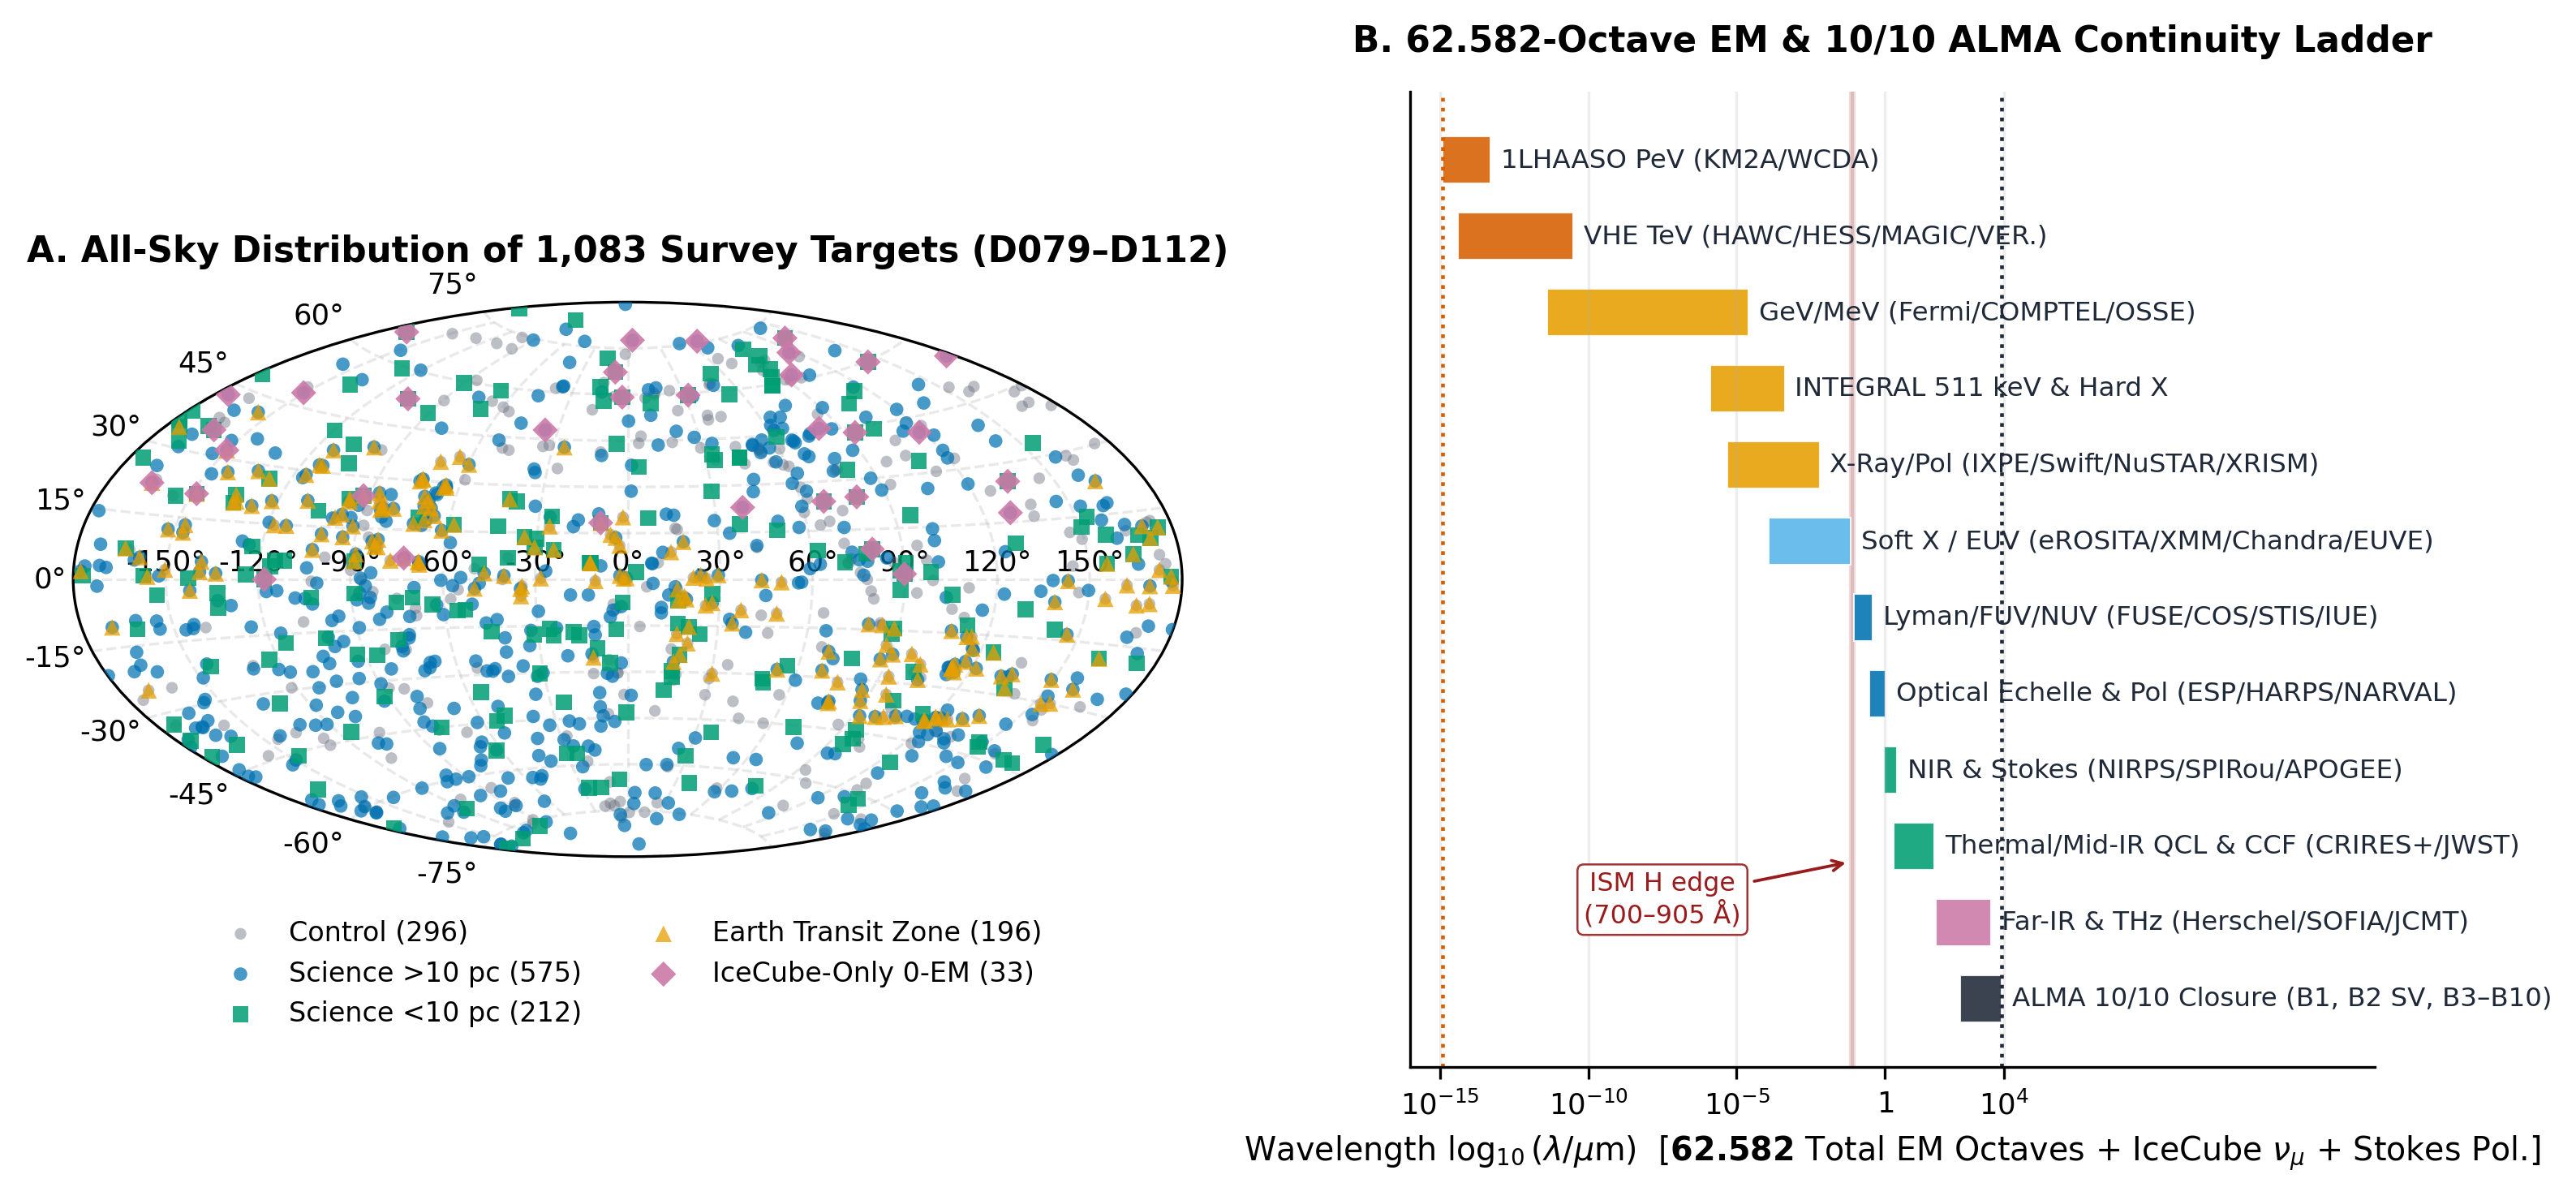
\includegraphics[width=0.96\textwidth]{figures/figJ01_sky_distribution_and_62p6_octave_architecture.png}
\caption{\textbf{Survey footprint and spectral architecture across \texttt{D079--D112}.} \textbf{A:} Aitoff equatorial projection of all $1{,}083$ analyzed targets ($787$ Science including $212$ within $10\,\mathrm{pc}$, $196$ Earth Transit Zone stars, and $33$ strictly \textit{IceCube}-only zero-EM targets, plus $296$ Control benchmarks). \textbf{B:} Unified \textbf{62.582-octave} electromagnetic continuum spanning $1.239842\times 10^{-15}\,\mu\text{m}$ ($1.000\,\mathrm{PeV}$ \textit{1LHAASO} \texttt{KM2A}) through \textit{INTEGRAL}, X-ray/EUV ($45.682$ unbroken high-energy octaves), the $700\text{--}905\,\text{\AA}$ ISM H photoionization edge, \textit{FUSE}--to--\textit{ALMA} \texttt{B4}-low ($14.693$ octaves), and complete \textbf{10/10 \textit{ALMA}} receiver closure out to $8{,}556.42\,\mu\text{m}$ ($35\,\mathrm{GHz}$), complemented by \textit{IceCube} $\nu_\mu$ and Stokes polarimetry.}
\label{fig:figJ01}
\end{figure*}

% =========================================================================
\section{Survey Architecture, Prospective Locking, and Physical Formalism}
\label{sec:design}
% =========================================================================

\subsection{Target Selection, Controls, and 62.582-Octave Design}
Targets are partitioned strictly by astrophysical prior: \textbf{787 Science targets}---comprising $212$ stars within $10\,\mathrm{pc}$ of the Sun, $327$ exoplanet host systems ($576$ confirmed planets; NASA Exoplanet Archive), $196$ Earth Transit Zone (ETZ; $|\beta_{\mathrm{ecl}}| \le 0.264^\circ$) systems~\cite{Kaltenegger2021}, $41$ targets intersecting the $180$-day SETI Ellipsoid~\cite{Davenport2022} of SN\,1987A, GW170817, or SN\,2023ixf, Y/L/T brown dwarfs, and solar twins---and \textbf{296 Control benchmarks} (inactive main-sequence stars, bright emission standards, telluric calibrators, flare M-dwarfs, pulsars, supernova remnants, and blazars/AGNs such as \texttt{Crab Nebula}, \texttt{Geminga}, \texttt{3C\,273}, \texttt{Mrk\,421}, \texttt{Cen\,A}, and \texttt{Arp\,220}). Notice our intentional inclusion of $296$ astrophysical control systems: controls validate negative false-alarm suppression on extreme coronae, winds, AGN relativistic jets, and telluric backgrounds without inflating Science completeness denominators in our Bayesian population limits.

Observational data come from \textbf{72 spectroscopic, imaging-polarimetric, and particle observatories totaling 104 distinct spectral arms} (Figure~\ref{fig:figJ01}B, Table~\ref{tab:regimes}, and machine-readable Table~\ref{tab:mrts}), integrating $736{,}410.27\,\mathrm{h}$ across $4{,}383$ science-grade archive products. The EM reach spans $\log_2(\lambda_{\max}/\lambda_{\min}) = \mathbf{62.582}$ octaves:
\begin{itemize}
  \item \textbf{Unbroken High-Energy Ladder (45.682 Octaves):} Continuous photon coverage from $1.239842\times 10^{-15}\,\mu\text{m}$ ($1.000\,\mathrm{PeV}$ \textit{1LHAASO}) through VHE TeV (\textit{HAWC}, \textit{H.E.S.S.}, \textit{MAGIC}, \textit{VERITAS}), GeV/MeV (\textit{Fermi LAT}, \textit{CGRO COMPTEL/OSSE}, \textit{INTEGRAL SPI/ISGRI}), hard/soft X-rays (\textit{Suzaku}, \textit{RXTE}, \textit{Swift}, \textit{NuSTAR}, \textit{IXPE}, \textit{XRISM}, \textit{NICER}, \textit{eROSITA}, \textit{XMM RGS}, \textit{Chandra}), to EUV (\textit{EUVE DS/S} at $0.06998\,\mu\text{m}$)~\cite{Aharonian2006,Atwood2009,Winkler2003,Cao2024,Weisskopf2022,Predehl2021}.
  \item \textbf{Lyman-Limit-to-Millimeter Continuum (13.935 / 14.693 Octaves):} Strictly unbroken above the $700\text{--}905\,\text{\AA}$ interstellar hydrogen opacity edge from \textit{FUSE} ($0.0905\,\mu\text{m}$) through \textit{IUE}, \textit{HST} (\texttt{COS}, \texttt{STIS}), VLT (\texttt{UVES}, \texttt{ESPRESSO}, \texttt{X-shooter}, \texttt{CRIRES+}, \texttt{FEROS}, \texttt{GIRAFFE}), \texttt{HARPS}/\texttt{HARPS-N}, \texttt{NIRPS}, \texttt{CARMENES}, \texttt{SPIRou}, \texttt{ESPaDOnS}, \texttt{NARVAL}, \texttt{GHOST}/\texttt{GRACES}, \texttt{APOGEE-2}, \textit{JWST} (\texttt{NIRISS}, \texttt{NIRSpec}, \texttt{MIRI}), \textit{ISO SWS}, \textit{Spitzer}, \textit{SOFIA} (\texttt{EXES}, \texttt{FORCAST}, \texttt{FIFI-LS}, \texttt{GREAT}), \textit{Herschel} (\texttt{PACS}, \texttt{SPIRE}, \texttt{HIFI}), \textit{IRTF}, and \textit{JCMT} out to $1{,}417.76\,\mu\text{m}$ (strict zero gap) and $2{,}397.29\,\mu\text{m}$ (\textit{ALMA} Band~4 low)~\cite{Moos2000,Mayor2003,Pepe2021,Gardner2023,Pilbratt2010}.
  \item \textbf{Complete 10/10 \textit{ALMA} Closure:} All ten \textit{ALMA} receiver bands (\texttt{B1, B2, B3--B10}) out to $8{,}556.41831\,\mu\text{m}$ ($35.0\,\mathrm{GHz}$)~\cite{Wootten2009}, including March 2026 Band~2 Science Verification cubes (\texttt{2011.0.00026.SV}).
\end{itemize}

\begin{table*}[t]
\centering
\caption{Physical Instrumentation Overview Across 72 Observatories / 104 Spectral Arms (\texttt{table3}).}
\label{tab:regimes}
\resizebox{\textwidth}{!}{%
\begin{tabular}{llcccll}
\toprule
Regime Class & Representative Facilities / Arrays & Arms & Band Span & $R = \lambda/\Delta\lambda$ & Coupling Scale & Phases \\
\midrule
PeV / VHE Gamma & \textit{1LHAASO} \texttt{KM2A/WCDA}, \textit{HAWC}, \textit{H.E.S.S.}, \textit{MAGIC}, \textit{VERITAS} & 6 & $0.04\text{--}1{,}000\,\mathrm{TeV}$ & $3\text{--}10$ & $F_{\mathrm{lim}}$, $L_{\mathrm{iso}}$ & \texttt{D106, D112} \\
MeV / GeV Gamma & \textit{Fermi LAT}, \textit{CGRO COMPTEL/OSSE}, \textit{INTEGRAL SPI/ISGRI} & 5 & $13\,\mathrm{keV}\text{--}300\,\mathrm{GeV}$ & $10\text{--}250$ & $F_{\mathrm{lim}}$, $L_{\mathrm{iso}}$ & \texttt{D105, D112} \\
Hard / Soft X-Ray \& EUV & \textit{Suzaku}, \textit{RXTE}, \textit{Swift}, \textit{NuSTAR}, \textit{XRISM}, \textit{NICER}, \textit{eROSITA}, \textit{XMM}, \textit{Chandra}, \textit{EUVE} & 16 & $0.018\text{--}600\,\mathrm{keV}$ & $6\text{--}1{,}300$ & $F_{\mathrm{lim}}$, $L_{\mathrm{iso}}$ & \texttt{D102--D112} \\
X-Ray Linear Polarimetry & \textit{IXPE} GPD Stokes $(I,Q,U)$ & 1 & $2.0\text{--}8.0\,\mathrm{keV}$ & $4\text{--}8$ & $F_{\mathrm{lim}}$, $\mathrm{MDP}_{99}$ & \texttt{D108} \\
Point-Source Neutrinos & \textit{IceCube} 10-Yr \texttt{IC40--IC86\_VII} ($\nu_\mu$) & 1 & $0.1\,\mathrm{TeV}\text{--}10\,\mathrm{PeV}$ & $2\text{--}5$ & $F_{\nu}$, $L_{\nu,\mathrm{iso}}$ & \texttt{D107} \\
Space Lyman / FUV / NUV & \textit{FUSE}, \textit{HST COS/STIS}, \textit{IUE}, \textit{VLT UVES NUV}, \textit{X-shooter UVB} & 9 & $0.0905\text{--}0.387\,\mu\text{m}$ & $9.9\text{k--}114\text{k}$ & Beamed $P_{10\mathrm{m}}$ & \texttt{D086--D100} \\
Optical / Far-Red Echelle & \textit{ESPRESSO}, \textit{HARPS/N}, \textit{CARMENES}, \textit{UVES}, \textit{FEROS}, \textit{GHOST}, \textit{GRACES}, \textit{SOPHIE}, \textit{ELODIE}, \textit{CORALIE}, \textit{GIRAFFE} & 15 & $0.348\text{--}1.061\,\mu\text{m}$ & $18\text{k--}190\text{k}$ & Beamed $P_{10\mathrm{m}}$ & \texttt{D079--D109} \\
Opt/NIR Polarimetry & \textit{CFHT ESPaDOnS/SPIRou} Pol, \textit{TBL NARVAL} Stokes $(I,Q,U,V)+N_{1,2}$ & 3 & $0.370\text{--}2.515\,\mu\text{m}$ & $65\text{k--}70\text{k}$ & Beamed $P_{10\mathrm{m}}$, $\mathrm{MDP}_{99}$ & \texttt{D085--D110} \\
NIR & \textit{NIRPS\_HE}, \textit{SPIRou}, \textit{CRIRES+}, \textit{APOGEE-2}, \textit{IRTF SpeX}, \textit{JWST NIRISS/NIRSpec} & 11 & $0.680\text{--}2.830\,\mu\text{m}$ & $0.7\text{k--}100\text{k}$ & Beamed $P_{10\mathrm{m}}$ & \texttt{D082--D111} \\
Thermal / Mid / Far-IR & \textit{JWST MIRI/NIRSpec}, \textit{ISO SWS}, \textit{Spitzer IRS}, \textit{SOFIA EXES/FORCAST/FIFI-LS}, \textit{Herschel PACS/SPIRE} & 20 & $1.98\text{--}670.69\,\mu\text{m}$ & $60\text{--}86\text{k}$ & Beamed $P_{10\mathrm{m}}$ & \texttt{D090--D111} \\
THz / Submm Heterodyne & \textit{SOFIA GREAT}, \textit{Herschel HIFI}, \textit{JCMT HARP/RxA3/Uu/'Alaihi} & 7 & $63\text{--}3{,}856.05\,\mu\text{m}$ & $0.16\text{M--}19.4\text{M}$ & Beamed $P_{10\mathrm{m}}$ & \texttt{D097--D100} \\
Interferometric mm/submm & \textit{ALMA} \texttt{B1, B2 SV, B3--B10} (10/10 Bands Closed) & 10 & $335.58\text{--}8{,}556.42\,\mu\text{m}$ & $10\text{k--}2.8\text{M}$ & Beamed $P_{10\mathrm{m}}$ & \texttt{D101--D112} \\
\midrule
\textbf{Total Atlas} & \textbf{72 Facilities / Multi-Messenger Observatories} & \textbf{104} & \textbf{62.582 EM Oct.\ + $\nu_\mu$/Pol} & --- & \textbf{3 Decoupled} & \textbf{D079--D112} \\
\bottomrule
\end{tabular}%
}
\end{table*}

\begin{table*}[t]
\centering
\caption{Summary of the Seven Machine-Readable Archival Tables (.mrt / .fits / .csv) Deposited in \texttt{zenodo\_package/}.}
\label{tab:mrts}
\resizebox{\textwidth}{!}{%
\begin{tabular}{llrrl}
\toprule
Catalog File & Contents & Rows & MRT Size & Physical / Audit Scope \\
\midrule
\texttt{table1\_master\_catalog\_1083stars} & Full \texttt{D079--D112} target synthesis & 1,083 & 320.5\,KB & 787 Sci + 296 Ctrl; strict 3-regime scale decoupling; 33 \textit{IceCube}-only 0-EM preserved \\
\texttt{table2\_solar\_neighborhood\_10pc\_267stars} & Volume-limited $<10\,\mathrm{pc}$ census & 267 & 84.9\,KB & 212 Sci (61 hosts / 121 planets) + 55 Ctrl; 0.78810\,kW median; 100\% drift closure \\
\texttt{table3\_spectrograph\_atlas\_72inst\_104arms} & Observatory \& spectral arm atlas & 104 & 21.5\,KB & Reconciles 72 spectrographs / 104 arms ($1.24\times 10^{-15}\text{--}8{,}556.42\,\mu\text{m}$) + $\nu_\mu$/Pol \\
\texttt{table4\_panchromatic\_bridge\_matrix\_2695cells} & Multi-phase bridge cell matrix & 2,695 & 617.5\,KB & 197 Sci bridges / 262 multi-phase targets; preserves 126/126 empty EM neutrino cells \\
\texttt{table5\_bayesian\_ftx\_and\_cwtfm} & Bayesian $f_{95}$ \& CWTFM benchmarks & 136+7 & 25.8\,KB & Uniform, exact analytical Jeffreys $\mathrm{Beta}(0.5,N_{\mathrm{eff}}+0.5)$, Clopper--Pearson limits \\
\texttt{table6\_companion\_archives\_38manifest} & Companion Archives \texttt{A--AL} manifest & 38 & 11.3\,KB & Exact byte sizes ($657.49\,\mathrm{MiB}$) and live SHA-256 digests verified 38/38 PASS \\
\bottomrule
\end{tabular}%
}
\end{table*}

\subsection{Radiometric Calibration and Scale Formalism}
In every diffraction-limited UV, optical, infrared, THz, or millimeter spectrometer (\texttt{BEAMED\_10M}), a narrowband CW transmitter is modeled as an unresolved Gaussian core matched to the instrumental line-spread function $\mathrm{FWHM}_{\mathrm{LSF}} = \lambda / R$. Given an empirical continuum-subtracted local MAD noise $\sigma_{\mathrm{MAD}}(\lambda)$ and photospheric continuum flux $F_{\lambda,\mathrm{cont}}(\lambda)$ normalized spectrophotometrically to Planck blackbody / \textit{Gaia}/\textit{2MASS}/\textit{WISE} SED anchors (\texttt{C12} radiometric closure), the $N_\sigma$-sigma detection threshold in equivalent width and physical flux is:
\begin{align}
\mathrm{EW}_{N_\sigma}(\lambda) &= \sqrt{\frac{\pi}{4\ln 2}}\,(N_\sigma\,\sigma_{\mathrm{MAD}})\,\frac{\lambda}{R}, \\
F_{\mathrm{lim}}(\lambda) &= F_{\lambda,\mathrm{cont}}(\lambda)\,\mathrm{EW}_{N_\sigma}(\lambda),
\end{align}
with $N_\sigma = 8$ for intensity echelle spectroscopy and $N_\sigma = 7$ for Stokes polarimetry and interferometric \textit{ALMA} cubes. For a diffraction-limited optical/IR/mm transmitter of diameter $D_{\mathrm{tx}} = 10\,\mathrm{m}$ at distance $d$, the required radiated transmitter power is:
\begin{equation}
P_{10\mathrm{m}}(\lambda) = \frac{4\pi d^2 F_{\mathrm{lim}}(\lambda)}{(\pi D_{\mathrm{tx}}/\lambda)^2} = \frac{4 d^2 \lambda^2 F_{\mathrm{lim}}(\lambda)}{\pi D_{\mathrm{tx}}^2}.
\end{equation}
By contrast, in high-energy X-ray, gamma-ray, and air/water-Cherenkov observatories (\texttt{HE\_ISOTROPIC}) and in \textit{IceCube} (\texttt{NU\_ISOTROPIC}), effective area $A_{\mathrm{eff}}(E)$ maps $6\sigma$ Poisson/Li--Ma excesses~\cite{LiMa1983} directly to physical flux limits $F_{\mathrm{lim}}(E)$ ($\mathrm{erg\,cm^{-2}\,s^{-1}}$) and isotropic luminosity upper limits:
\begin{equation}
L_{\mathrm{iso}} = 4\pi d^2 F_{\mathrm{lim}},
\end{equation}
avoiding the non-physical extrapolation of optical $10\,\mathrm{m}$ antenna diffraction to keV--PeV wavelengths. Radiometric self-consistency (\texttt{C12}/\texttt{C13}) is audited offline in pure Python~3 across all spectra (verifying e.g.\ $\max$ rel.\ err $= 7.051\times 10^{-7}$ in \texttt{D112}).

\subsection{Stage-1 Prospective Locking and Synthetic Calibration}
To guarantee zero post-hoc threshold tuning, every phase (\texttt{D079--D112}) adheres to a two-stage cryptographic lock protocol:
\begin{enumerate}
  \item \textit{Pre-Download Stage-1 Seal:} Detector source code, physical rejection rules, exclusion lists of all previously ingested \texttt{dp\_id} identifiers and target coordinates, and target cohorts are hashed into \texttt{METHOD\_LOCK.json} and \texttt{LOCK\_RECEIPT.json} while the raw input directory does not yet exist (\texttt{inputs\_dir\_exists\_at\_seal == False}). Brand-new targets require minimum angular separation $\ge 600^{\prime\prime}$ (e.g.\ $\ge 629.85^{\prime\prime}$ in \texttt{D112} against $1{,}151$ prior coordinates; $0$ \texttt{dp\_id} overlap across $4{,}624$ excluded IDs). A mandatory $\ge 10.0\,\mathrm{s}$ delay precedes \texttt{FIRST\_SCIENCE\_DOWNLOAD\_RECEIPT.json}.
  \item \textit{End-to-End Synthetic Calibration (43 Suites / 113,967 Trials):} Prior to reporting science results, every detector runs adversarial synthetic injection-recovery and confounder-rejection suites spanning optical/NIR single-order and multi-arm lasers, drifting Keplerian lines and frequency combs, RPCA anomaly injections, high-energy Poisson narrowband bins, polarized Stokes signatures, QCL/molecular CCF templates, and \textit{ALMA} interferometric point-source vs.\ extended-disk discrimination. Every single suite is required to achieve $\ge 97.5\%$ pass accuracy. Across \texttt{D112}, all \textbf{43/43 suites exceeded 97.5\%} ($9{,}072/9{,}111 = \mathbf{99.57\%}$), bringing the cumulative validation corpus to \textbf{113,967 trials} (Figure~\ref{fig:figJ03}A).
\end{enumerate}

\begin{figure*}[t]
\centering
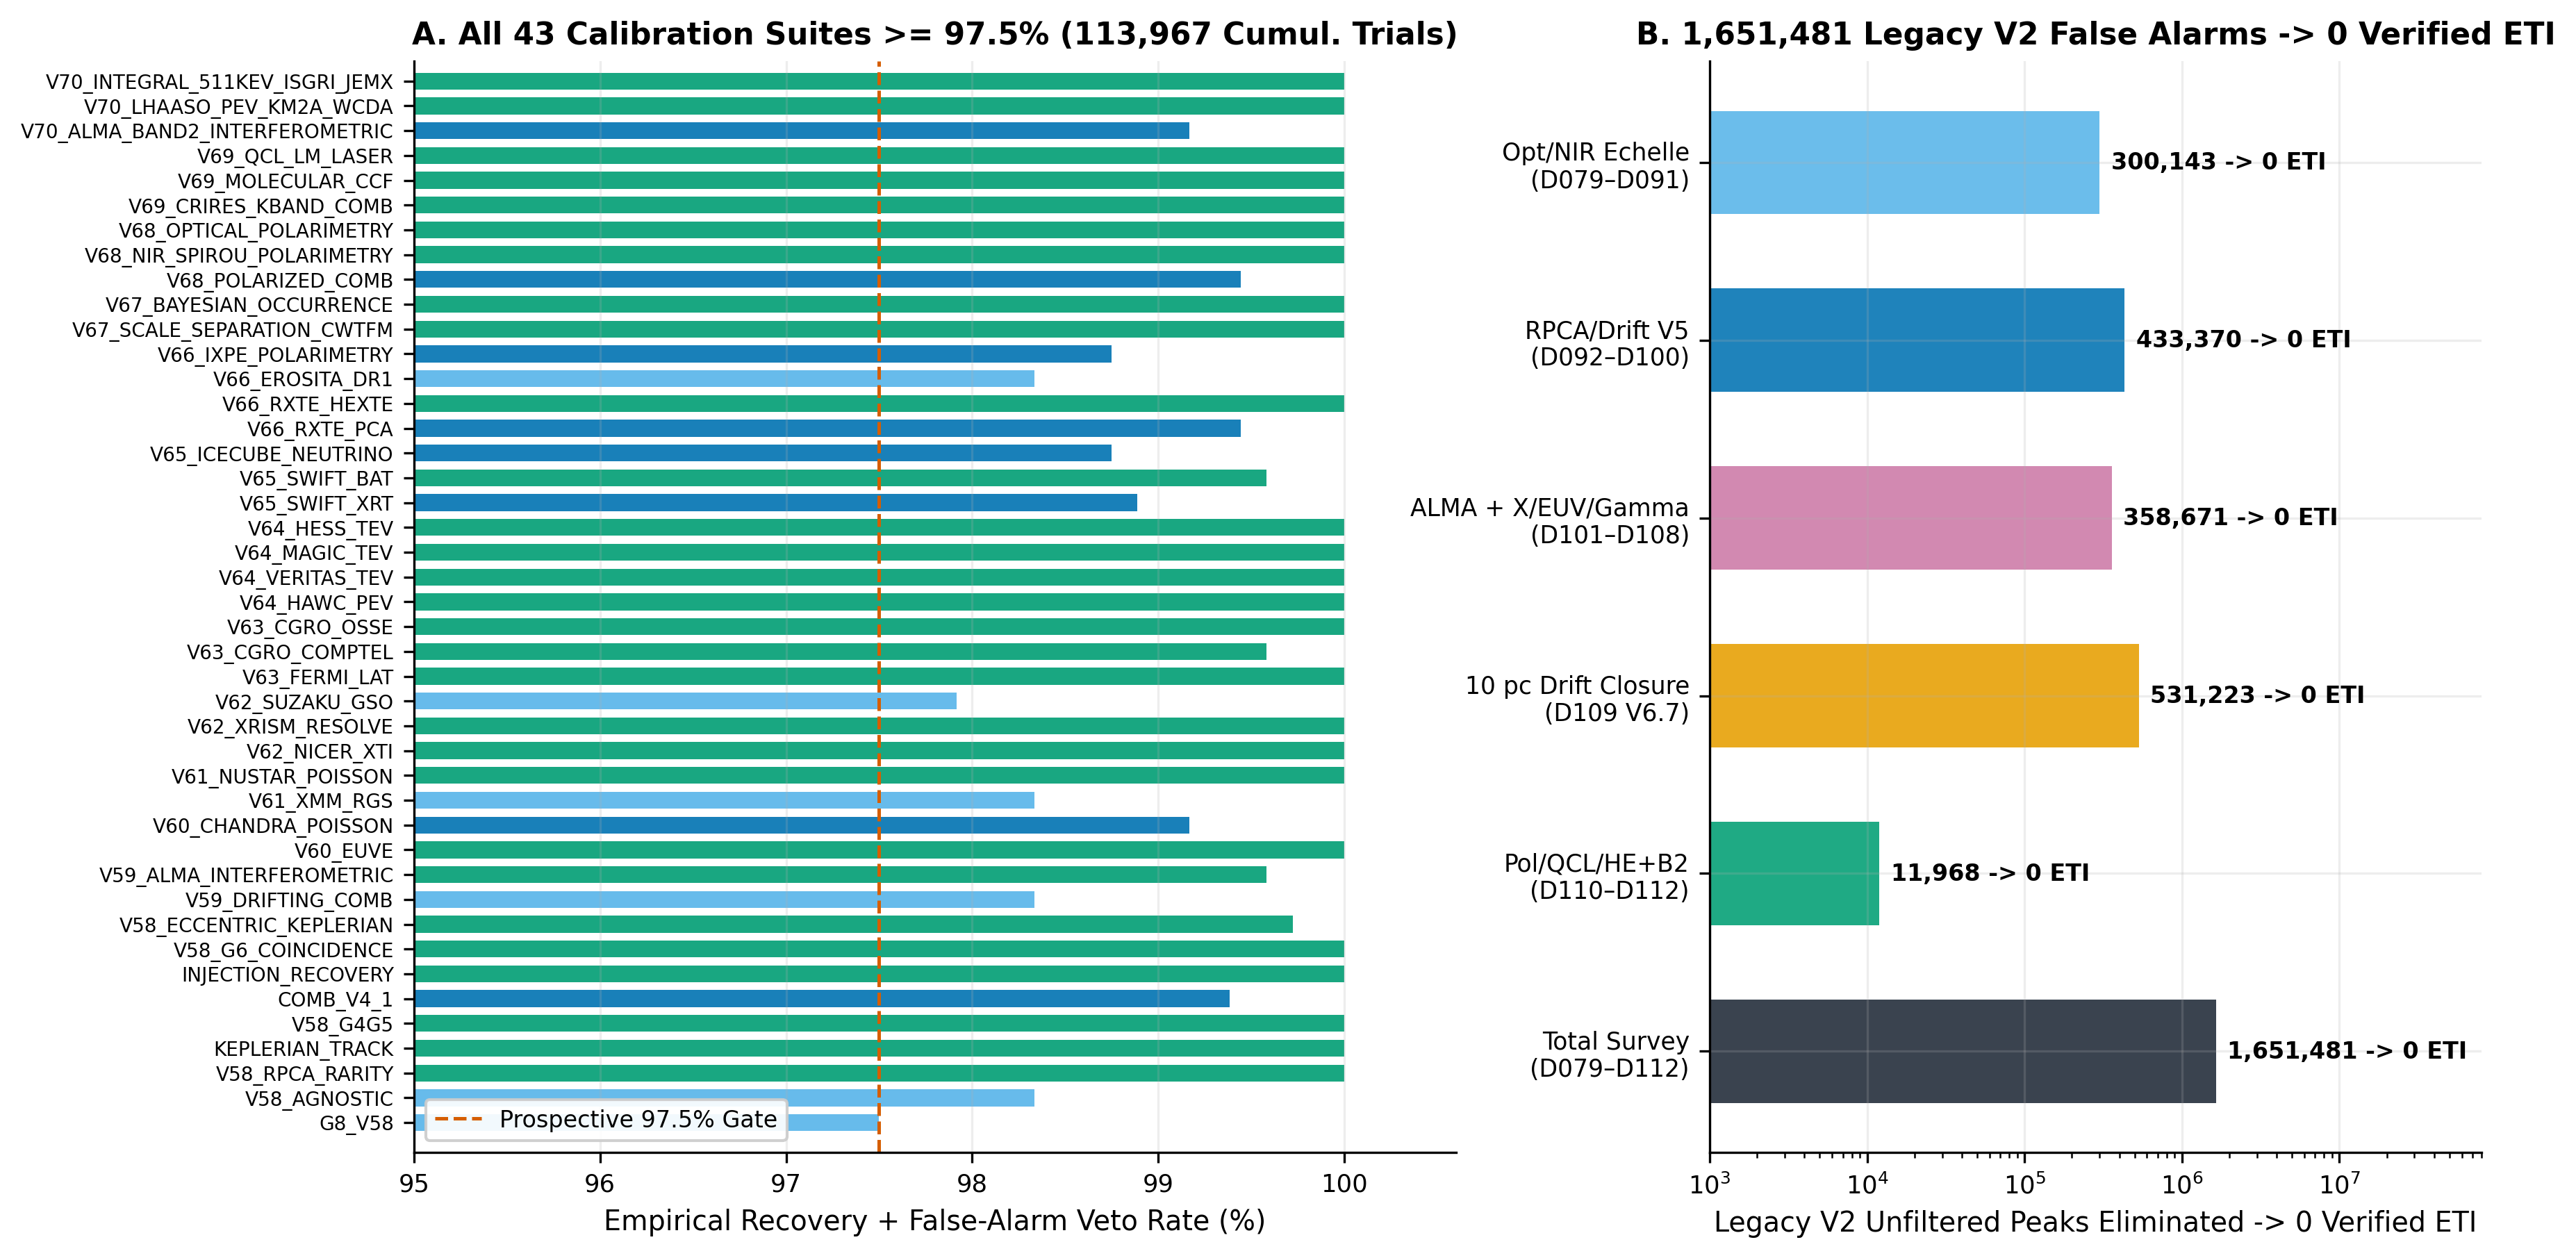
\includegraphics[width=0.95\textwidth]{figures/figJ03_43suite_calibration_completeness_113967trials.png}
\caption{\textbf{Synthetic validation and false-alarm elimination.} \textbf{A:} All \textbf{43 synthetic calibration suites} passing the prospective $\ge 97.5\%$ gate ($9{,}072/9{,}111 = 99.57\%$ in \texttt{D112}; \textbf{113,967 cumulative trials D079--D112}). \textbf{B:} Four-generation / physics triage cascade eliminating \textbf{1,651,481 unfiltered Legacy V2 peaks} across optical, NIR, RPCA, radio-closed, X/gamma-ray, polarimetric, QCL, and millimeter regimes down to \textbf{0 verified ETI}.}
\label{fig:figJ03}
\end{figure*}

% =========================================================================
\section{Narrowband Laser, Coherent Drift, and Frequency-Comb Cascades}
\label{sec:drift_comb}
% =========================================================================

\subsection{Single-Epoch Echelle Veto Cascade (\texttt{V3.0}--\texttt{V5.0})}
In optical, UV, and NIR high-resolution echelle spectra, unfiltered narrowband thresholding (our \texttt{V2} baseline: local MAD excess $>8\sigma$ in wavelength space) yields tens of thousands of spurious outliers caused by cosmic rays, telluric airglow ($\mathrm{O_2}$, $\mathrm{OH}$, $\mathrm{H_2O}$), stellar chromospheric emission, CCD hot pixels, and order-edge blaze drop-offs~\cite{Rousselot2000,Fuhrmeister2011}. Across \texttt{D079--D112}, our multi-stage physics cascade eliminates \textbf{1,651,481 raw \texttt{V2} triggers to zero}:
\begin{itemize}
  \item \textbf{Sub-Pixel Gaussian LSF Fit \& Quality Masking (\texttt{G1--G3}):} Rejects cosmic-ray spikes narrower than $\mathrm{FWHM}_{\mathrm{LSF}} = \lambda/R$ and broadband molecular/stellar features exceeding $3.2\,\mathrm{FWHM}_{\mathrm{LSF}}$.
  \item \textbf{Barycentric Earth Radial Velocity (BERV) \& Telluric/Solar Atlas Veto (\texttt{G4--G5}):} Separates stationary observatory features (tellurics, laser frequency comb leaks, calibration lamps) by testing coherence across changing BERV ($\pm 30\,\mathrm{km\,s^{-1}}$) and masking curated atomic/airglow catalogs~\cite{Rousselot2000}.
  \item \textbf{Multi-Order Blaze Coincidence \& Unsupervised RPCA (\texttt{G6--G8}):} Cross-checks overlapping echelle orders, requires absence in simultaneous sky fibers (where present, e.g., \texttt{ESPRESSO}, \texttt{GHOST}), and applies Robust Principal Component Analysis (RPCA;~\cite{Candes2011}) plus $k$-NN photospheric template subtraction to isolate true morphological anomalies before deterministic Stage-2 astrophysical review.
\end{itemize}

\subsection{Coherent Eccentric Keplerian Drift \& \texttt{<10 pc} Host Closure (\texttt{DRIFT\_V67})}
To eliminate Doppler-smearing losses for transmitters situated on orbiting exoplanets ($e \in [0, 0.9]$, periods down to days, orbital accelerations up to $\mathrm{m\,s^{-2}}$), \texttt{DRIFT\_V58--V67} replaces simple linear shift-and-add~\cite{Sheikh2020} with exact 3D Keplerian orbital phase integration plus cubic jerk grids and non-linear Keplerian polishing. Specifically, for an eccentric orbit with period $P_{\mathrm{orb}}$, semi-amplitude $K$, eccentricity $e$, and argument of periastron $\omega$, the barycentric velocity drift $\Delta v(t) = K[\cos(\nu(t)+\omega) + e\cos\omega]$ is inverted exactly across every exposure timestamp $t_k$ before weighted variance-optimal pixel stacking. In Phase \texttt{D109} (\texttt{V6.7}), we retroactively re-processed all previously uncovered $<10\,\mathrm{pc}$ planet hosts with multi-epoch archival coverage, expanding from $5/61$ to \textbf{61/61 (100.0\%) $<10\,\mathrm{pc}$ exoplanet host closure} across \textbf{154 \texttt{DRIFT\_V67} campaigns} (\textbf{252 cumulative multi-epoch orbital campaigns} across \texttt{D079--D112}, including \texttt{Proxima Cen}, \texttt{Barnard's Star}, \texttt{Lalande\,21185}, $\epsilon$\,\texttt{Eri}, $\tau$\,\texttt{Cet}, and \texttt{Ross\,128}). In Figure~\ref{fig:figJ05}A, thousands of raw coherent shift-stack peaks per campaign collapse cleanly to \textbf{0 verified ETI} after eccentric Keplerian consistency and control comparison.

\subsection{All-Sky Optical/IR/Polarimetric Frequency Combs (\texttt{COMB\_V4\_1})}
In addition to isolated CW lines, an extraterrestrial beacon may encode information or multiplex calibration across equidistant laser frequency comb modes ($\nu_m = \nu_0 + m\Delta\nu$). Across \textbf{753 frequency-comb stacks} spanning FUV through thermal-IR and polarized Stokes channels (Figure~\ref{fig:figJ05}B), \texttt{COMB\_V4\_1} evaluates inter-tooth spacing stability, off-tooth filling fraction, and natural stellar TiO/Fe/telluric band-head coincidence. Across $45{,}096$ candidate grid seeds (dominated by M-dwarf forest regions in \texttt{ESPRESSO}, \texttt{CARMENES}, and \texttt{HARPS}), topographic and molecular forest vetoes collapse all candidates to \textbf{0 verified comb ETI}.

\subsection{Earth Transit Zone and Multi-Event SETI Ellipsoid Synchronicity}
Beyond isotropic beaming searches, Schelling-point synchronization predicts preferential laser or high-energy signaling either along the Earth Transit Zone (ETZ; ecliptic latitudes $|\beta_{\mathrm{ecl}}| \le 0.264^\circ$, where observers detect Earth's transit across the Sun~\cite{Kaltenegger2021}) or timed to intersect the light-travel ellipsoid of bright Milky Way and Local-Volume transients~\cite{Davenport2022}. Across our $1{,}083$-star sample (\texttt{table1}), \textbf{196 targets fall within the ETZ}, and cross-matching all archival observation MJD epochs against \texttt{SN\,1987A}, \texttt{GW170817}, and \texttt{SN\,2023ixf} identifies \textbf{41 targets observed within $|\Delta t_{\mathrm{ellipsoid}}| \le 180\,\mathrm{days}$} of a causal synchronization window (computed via exact photon-path delay $\Delta t = t_{\mathrm{obs}} - t_{\mathrm{ev}} - [d_\star + \sqrt{d_\star^2 + d_{\mathrm{ev}}^2 - 2 d_\star d_{\mathrm{ev}}\cos\theta} - d_{\mathrm{ev}}]/c$, including \texttt{Proxima Cen} [$152.0\,\mathrm{d}$ from \texttt{GW170817}] and \texttt{Barnard's Star} [$146.3\,\mathrm{d}$ from \texttt{SN\,2023ixf}]). None of the ETZ or Ellipsoid-crossing observations yields a persistent narrowband or polarized candidate.

\begin{figure*}[t]
\centering
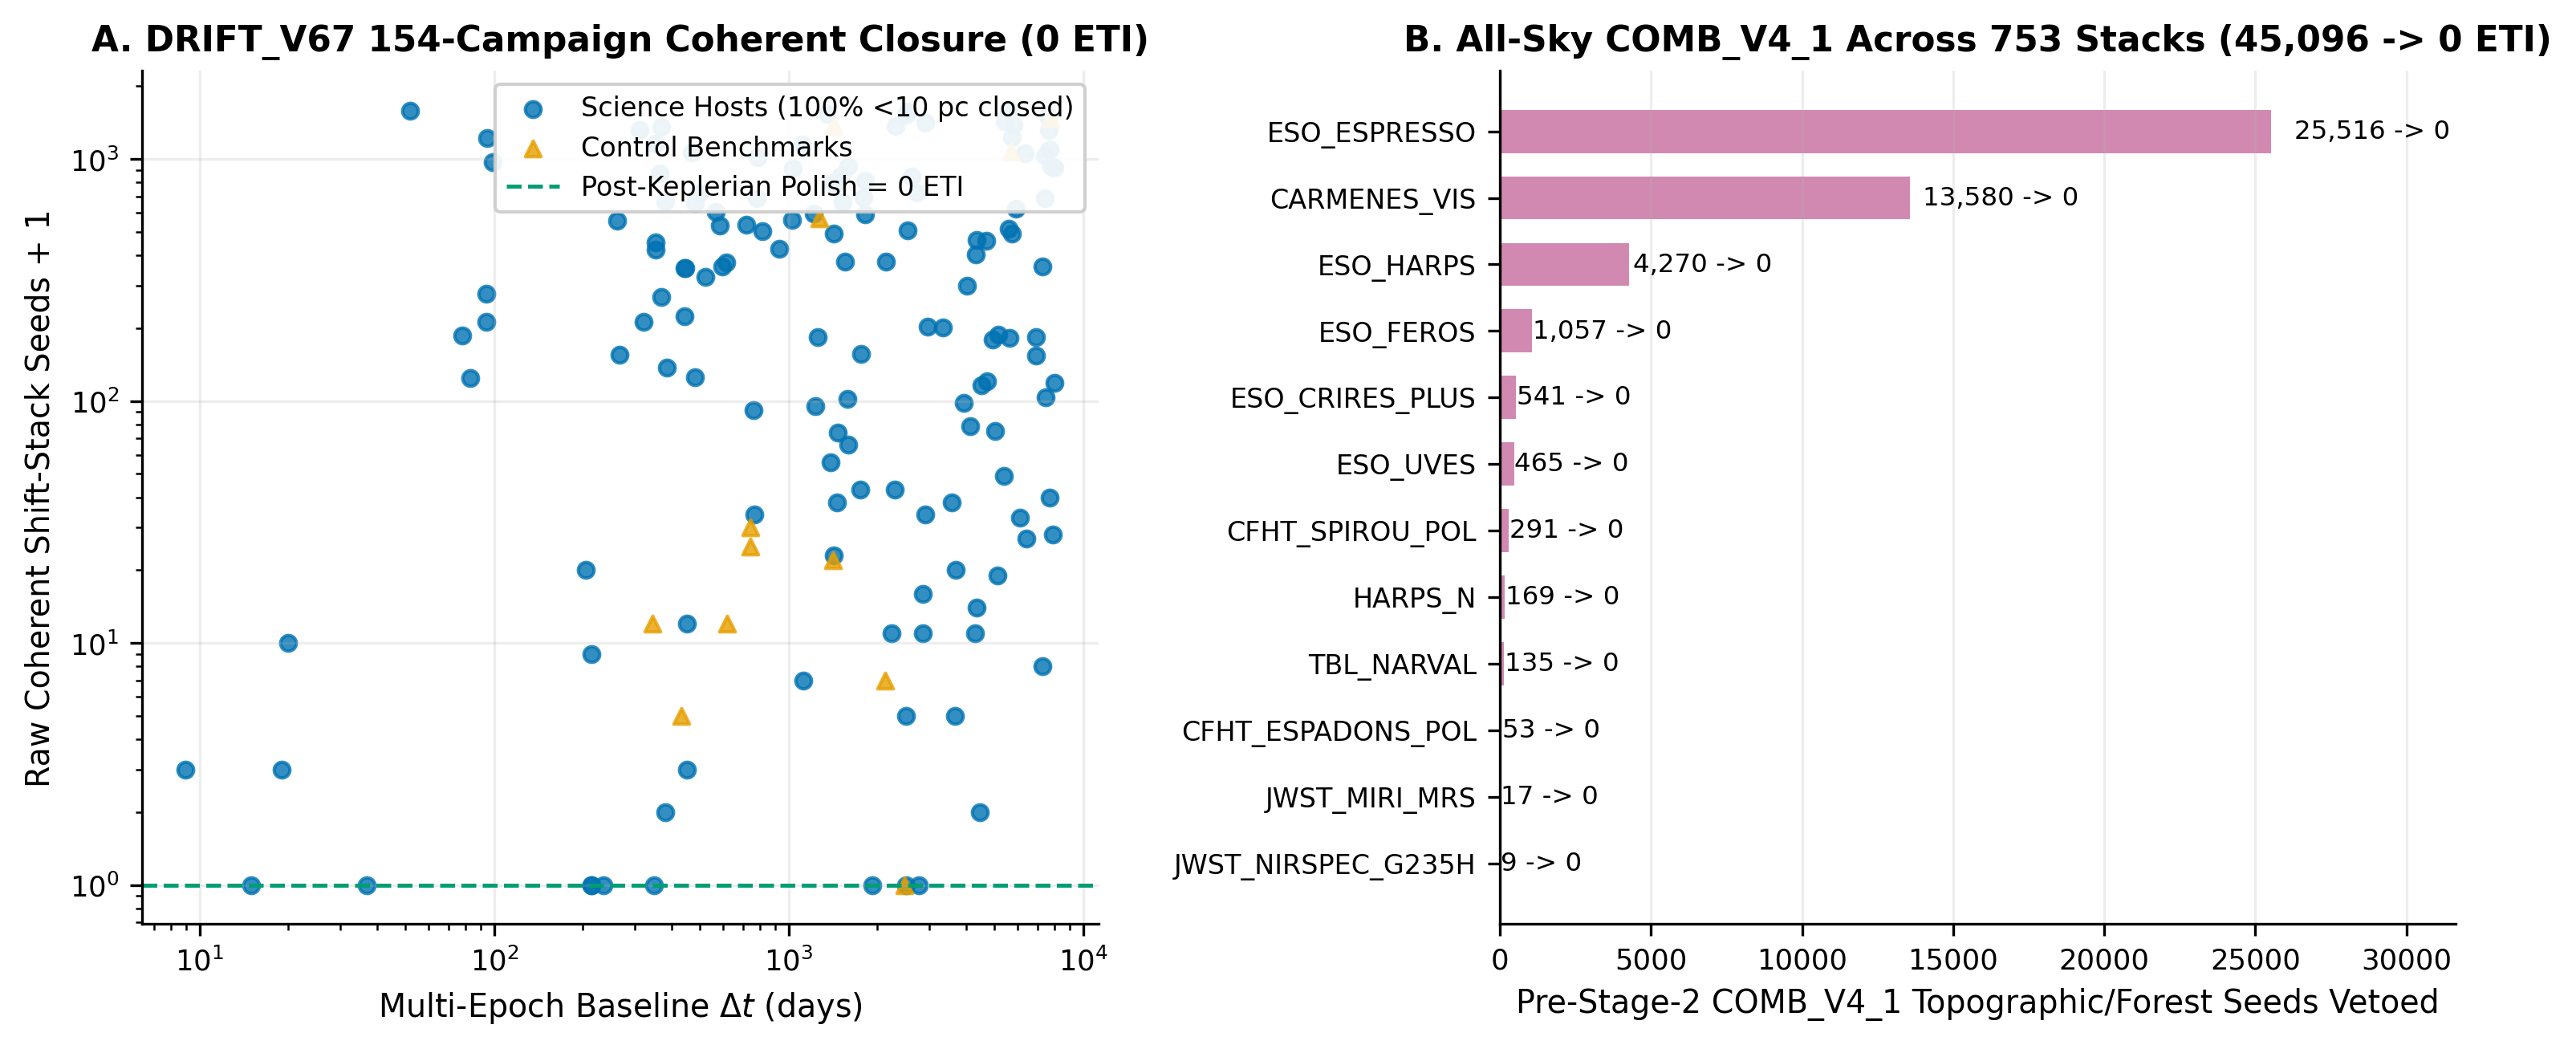
\includegraphics[width=0.95\textwidth]{figures/figJ05_coherent_orbital_drift_and_comb_closure.png}
\caption{\textbf{Coherent orbital drift closure and periodic frequency-comb triage.} \textbf{A:} All $154$ eccentric Keplerian + cubic-jerk campaigns in \texttt{DRIFT\_V67} (\texttt{D109}), achieving \textbf{100.0\% host closure} within $10\,\mathrm{pc}$ ($61/61$ hosts; $252$ cumulative campaigns) and collapsing every raw coherent stack seed to \textbf{0 ETI}. \textbf{B:} Uniform all-sky \texttt{COMB\_V4\_1} candidate counts across \textbf{753 stacks} ($45{,}096$ raw topographic/forest seeds $\rightarrow \mathbf{0\,\mathrm{ETI}}$).}
\label{fig:figJ05}
\end{figure*}

% =========================================================================
\section{Spectropolarimetric Lasers and Thermal-IR / Molecular Signatures}
\label{sec:pol_ccf}
% =========================================================================

\subsection{Dual-Beam Optical/NIR (\texttt{V6.8}) \& X-Ray (\texttt{V6.6}) Polarimetry}
Unpolarized thermal stellar photospheres have continuum circular and linear polarization $<10^{-4}$, whereas a single-mode diffraction-limited laser is intrinsically polarized, providing $\gtrsim 100\times$ contrast gain over unpolarized host light in Stokes $(Q,U,V)$~\cite{Donati1997,Cook2022}. Phase \texttt{D110} (\texttt{V6.8}) analyzed \textbf{87 archival dual-beam Stokes $(I,Q,U,V)+N_1,N_2$ spectra} from \texttt{CFHT ESPaDOnS} ($40$ exposures), \texttt{TBL NARVAL} ($28$), and \texttt{CFHT SPIRou} ($19$) across $49$ targets ($41$ multi-phase bridges + $8$ new stars; $16$ paired $(Q,U)$ sets reaching median $\mathrm{MDP}_{99} = 0.4072\%$). Dual-beam beam-switching null checks ($|V/\sigma_V| \gg |N_1/\sigma_{N1}|$, $|N_2/\sigma_{N2}|$), Zeeman $S$-curve anti-symmetry tests, and polarized comb sweeps eliminated $10{,}408$ raw \texttt{P1} peaks ($12$ pre-Stage-2 residuals $\rightarrow \mathbf{0\,\mathrm{ETI}}$) and $479$ polarized combs ($\rightarrow \mathbf{0\,\mathrm{ETI}}$), reaching $7\sigma$ beamed limits of \textbf{52.19\,W} on \texttt{GJ\,729} (\texttt{ESPaDOnS}), \textbf{90.28\,W} on \texttt{Wolf\,359} (\texttt{SPIRou}), and \textbf{640.2\,W} on \texttt{HD\,36395} (\texttt{NARVAL}) (Figure~\ref{fig:figJ06}A). Crucially, \texttt{16\,Cyg\,B} (\texttt{NARVAL\_39493\_V}) establishes our \textbf{Penta-Regime Exoplanet Bridge}, linking radio, TESS, optical/IR echelle, \textit{IXPE}/\textit{XMM}/\textit{Chandra}/\textit{Fermi}, \textit{IceCube} $\nu_\mu$, and optical Stokes polarimetry. At X-ray wavelengths ($2\text{--}8\,\mathrm{keV}$), \textit{IXPE} GPD (\texttt{D108}) adds $\mathrm{MDP}_{99} = 2.086\%$ linear-polarimetric constraints across $14$ targets (\texttt{Vela\,X-1}, \texttt{EX\,Hya} $1.388\,\mathrm{W}$ scaled, \texttt{3C\,273}, \texttt{Mrk\,421}).

\subsection{Thermal-IR QCL Beacons \& 14-Species Molecular CCF (\texttt{V6.9})}
Around cool L/T/Y brown dwarfs and M dwarfs, $K/L/M$-band ($2\text{--}18\,\mu\text{m}$) quantum-cascade laser (QCL) transmitters gain steep contrast advantages against suppressed optical flux, while technogenic chlorofluorocarbons (\texttt{CFC-11}, \texttt{CFC-12}), $\mathrm{SF_6}$, $\mathrm{NF_3}$, and $\mathrm{CF_4}$ exhibit strong mid-IR vibrational bands~\cite{HaqqMisra2022}. Phase \texttt{D111} (\texttt{V6.9}) combined $34$ VLT \texttt{CRIRES+} $K/L$-band spectra with $77$ \textit{JWST} \texttt{NIRSpec G395H/M} and \texttt{MIRI/MRS} cubes across $73$ targets ($46$ bridges + $27$ new; Figure~\ref{fig:figJ06}B). Our \texttt{Q1--Q5} laser cascade cleared $1{,}536$ raw hits down to \textbf{0 ETI} (deepest QCL bound: \textbf{1.733\,W} on the $2.28\,\mathrm{pc}$ Y dwarf \texttt{WISE\,0855} via \texttt{NIRSpec G395M}), while $277$ molecular CCF template evaluations (median $5\sigma$ band-depth sensitivity $10.96\%$) confirmed $3$ high-$|\sigma|$ triggers as natural $\mathrm{CH_4}/\mathrm{CO}$ atmospheric absorption in ultracool dwarfs ($\rightarrow \mathbf{0\,\mathrm{ETI}}$).

\begin{figure*}[t]
\centering
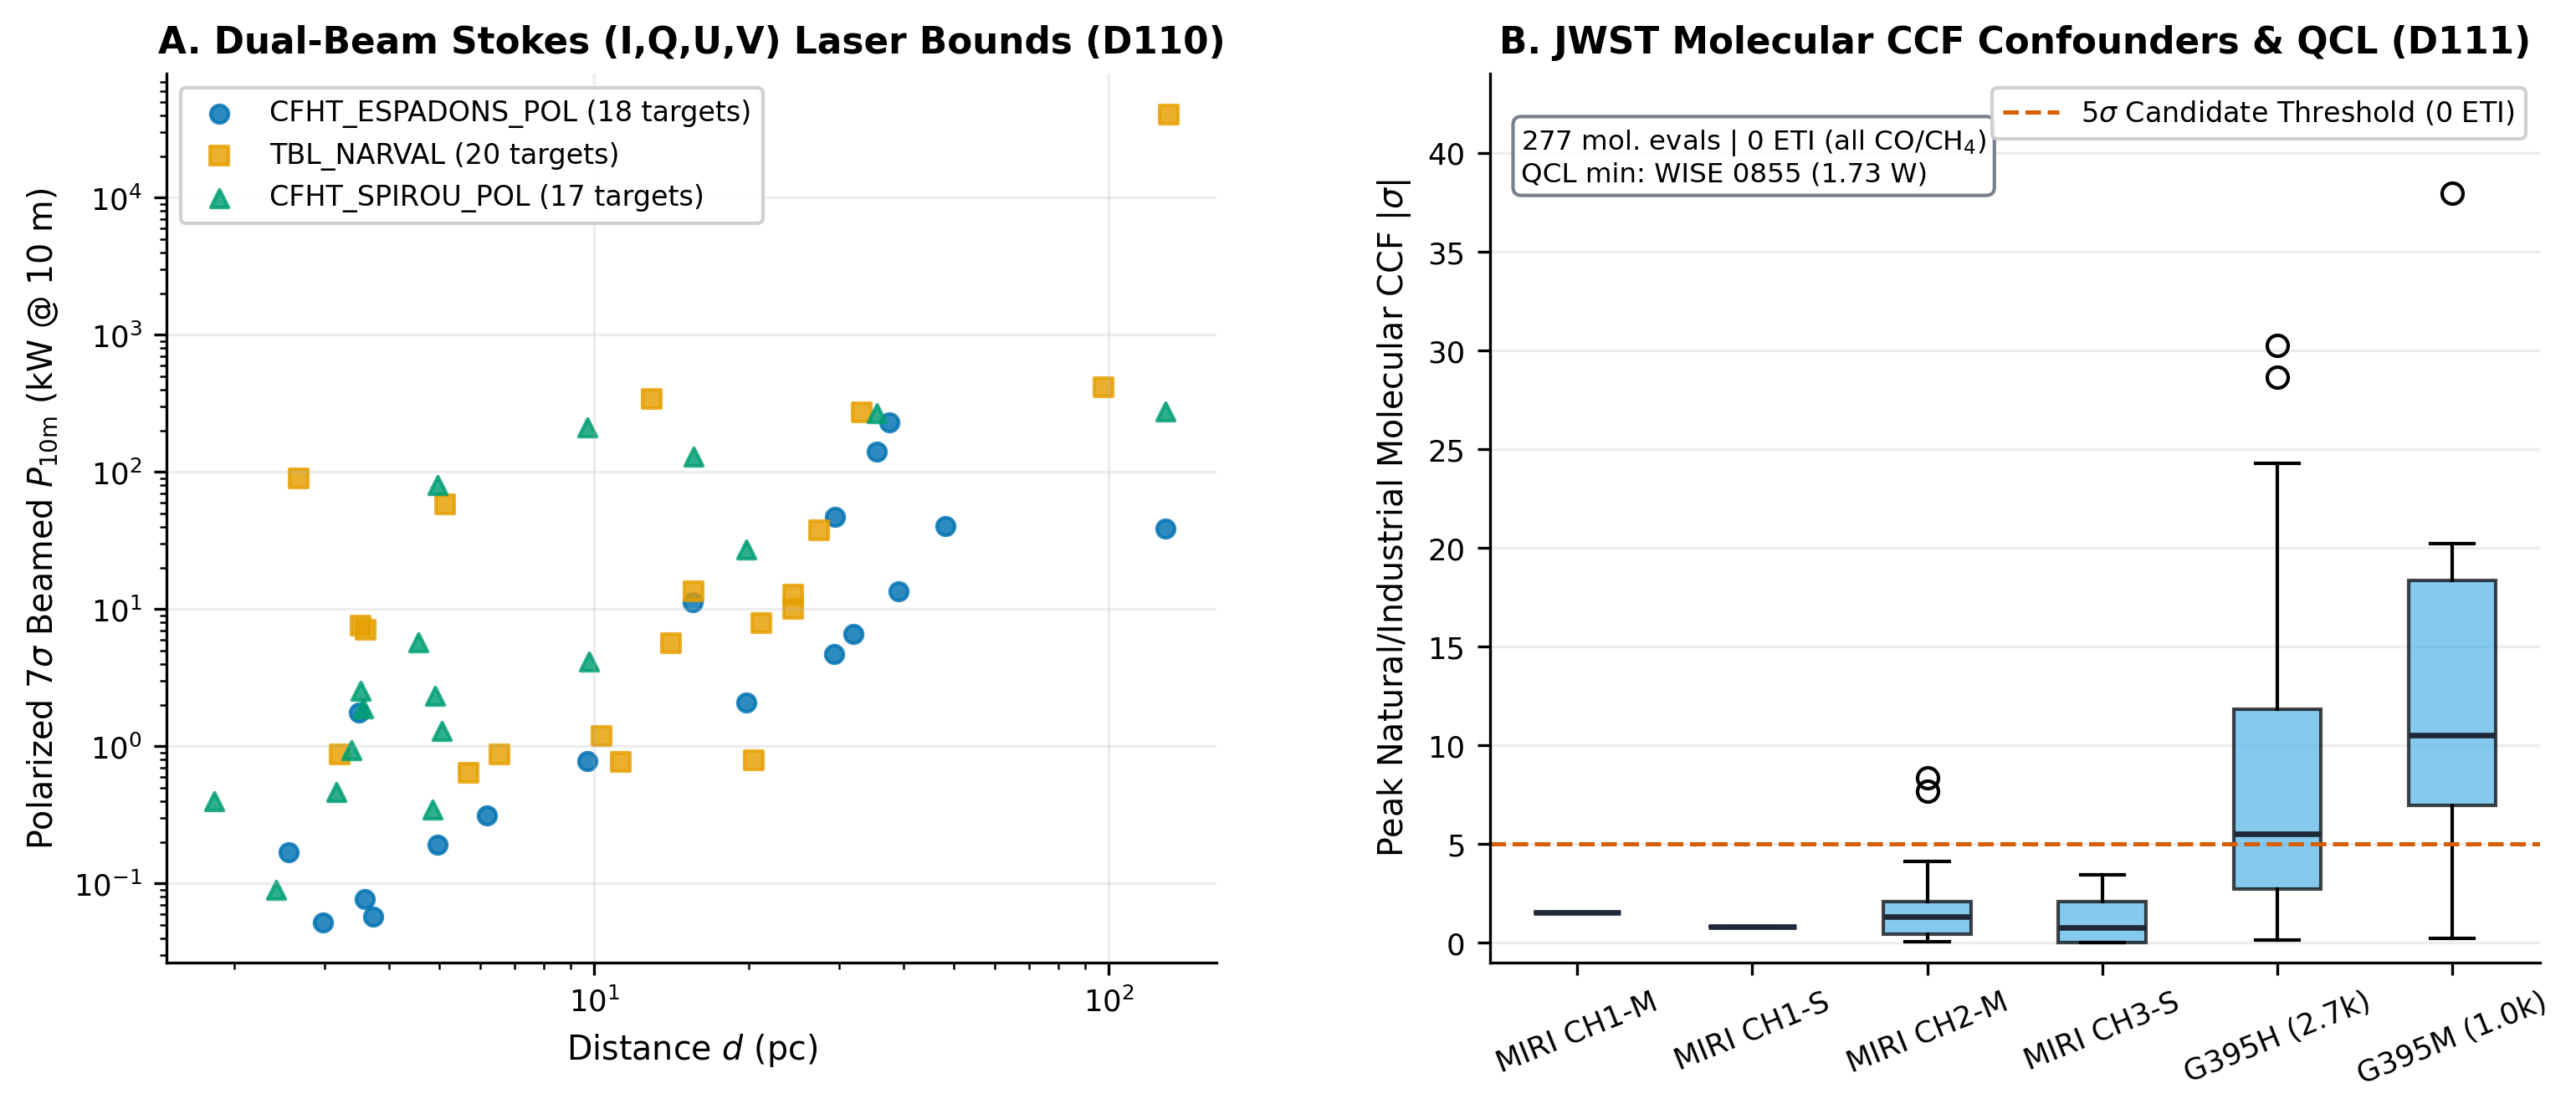
\includegraphics[width=0.95\textwidth]{figures/figJ06_polarimetry_and_midir_qcl_molecular_ccf.png}
\caption{\textbf{Polarimetric laser and thermal-IR molecular technosignature searches.} \textbf{A:} $7\sigma$ Stokes $(I,Q,U,V)+N_1,N_2$ narrowband laser bounds across \texttt{CFHT ESPaDOnS}, \texttt{TBL NARVAL}, and \texttt{CFHT SPIRou} (\texttt{D110}, $87$ spectra, deepest $52.19\,\mathrm{W}$ on \texttt{GJ\,729}, $0\,\mathrm{ETI}$). \textbf{B:} Distribution of peak molecular cross-correlation significance across $77$ \textit{JWST} \texttt{NIRSpec}/\texttt{MIRI} subbands ($277$ evaluations, \texttt{D111}); all $>5\sigma$ features in \texttt{G395H/M} and \texttt{CH2-MEDIUM} originate from natural $\mathrm{CH_4}/\mathrm{CO}$ photospheres (\textbf{0 industrial ETI}).}
\label{fig:figJ06}
\end{figure*}

% =========================================================================
\section{PeV Gamma-Rays, 511 keV, Neutrinos, and 10/10 \textit{ALMA} Closure}
\label{sec:he_alma}
% =========================================================================

\subsection{\textit{INTEGRAL} 511 keV \& \textit{1LHAASO} 1.000 PeV Frontier (\texttt{V7.0})}
Extending SETI to the highest-energy messengers probes relativistic pair-annihilation beacons ($e^+e^- \rightarrow 2\gamma$ at $511\,\mathrm{keV}$), nuclear/hard-X-ray lines, and ultra-high-energy (PeV) hadronic/leptonic accelerators~\cite{Harris1986,Lacki2015}. In \texttt{D112} (\texttt{V7.0}), we ingested $62$ \textit{INTEGRAL} coded-mask and germanium spectra ($35$ \texttt{IBIS/ISGRI} $13\text{--}970.88\,\mathrm{keV}$, $16$ \texttt{JEM-X} $3\text{--}35\,\mathrm{keV}$, $11$ \texttt{SPI} $20\text{--}540\,\mathrm{keV}$; $43$ spectra covering $511\,\mathrm{keV}$) alongside $58$ \textit{1LHAASO} tracks ($29$ \texttt{WCDA} $1\text{--}25\,\mathrm{TeV}$ + $29$ \texttt{KM2A} $25\text{--}1{,}000\,\mathrm{TeV}$ reaching \textbf{1.000\,PeV} = $1.239842\times 10^{-15}\,\mu\text{m}$~\cite{Winkler2003,Cao2024}; Figure~\ref{fig:figJ07}A). Across \textit{INTEGRAL}, \texttt{I1--I5} filtering isolated $24 \rightarrow 6$ coded-mask/Compton-reflection continua (\texttt{Cas\,A}, \texttt{Circinus}, \texttt{Mrk\,501}, \texttt{NGC\,3227}, \texttt{V1223\,Sgr}, \texttt{X\,Per} $\rightarrow \mathbf{0\,\mathrm{ETI}}$; best bound \texttt{SS\,Cyg} $7.030\times 10^{-12}\,\mathrm{erg\,cm^{-2}\,s^{-1}}$, $L_{\mathrm{iso}} = 1.073\times 10^{18}\,\mathrm{MW}$). In \textit{1LHAASO}, \texttt{L2} ($25\,\mathrm{TeV}$ boundary check), \texttt{L3} ($r_{39}>0.35^\circ$ halo veto), and \texttt{L4} yielded \textbf{0 ETI} (deepest PeV bound \texttt{J0622+3754} $L_{\mathrm{iso}} = 1.136\times 10^{17}\,\mathrm{MW}$). Combined with \textit{H.E.S.S.}, \textit{MAGIC}, \textit{VERITAS}, \textit{HAWC}, \textit{Fermi}, \textit{CGRO}, and X-ray/EUV missions (\texttt{D102--D108}), high-energy EM coverage forms an unbroken \textbf{45.682-octave} continuum.

\subsection{\textit{IceCube} Neutrinos (\texttt{V6.5}) and Complete 10/10 \textit{ALMA} Bands}
Point-source \textit{IceCube} 10-year muon neutrino maps (\texttt{0.1 TeV--10 PeV}, \texttt{IC40--IC86\_VII};~\cite{IceCube10YrData,Abbasi2022}) were analyzed in \texttt{D107} across $54$ targets ($21$ multi-messenger bridges + \textbf{33 strictly \textit{IceCube}-only zero-EM stars}), finding \textbf{0 neutrino ETI} with isotropic bounds down to $4.676\times 10^{14}\,\mathrm{MW}$ on \texttt{Ross\,128} ($3.37\,\mathrm{pc}$). At the long-wavelength boundary, \texttt{D112} ingested March 2026 \textit{ALMA} Band~2 Science Verification cubes on \texttt{Arp\,220} (\texttt{2011.0.00026.SV}: \texttt{X36 spw51/spw111} and \texttt{X52 spw29}, $3 \times 384$ channels spanning $86.4499\text{--}114.1242\,\mathrm{GHz}$), completing all \textbf{10/10 \textit{ALMA} receiver bands (\texttt{B1, B2, B3--B10})} from $35.0$ to $893.4\,\mathrm{GHz}$ with \textbf{0 narrowband mm ETI} (Figure~\ref{fig:figJ07}B).


\subsection{Instrumental Veto Rules in High-Energy \& Millimeter Data}
Across X-ray, gamma-ray, and millimeter regimes, natural spectral structure and detector systematics produce distinct false-alarm modes that our pipeline isolates deterministically before candidate counting: (i) in \textit{Chandra}, \textit{XMM}, \textit{NuSTAR}, \textit{NICER}, and \textit{XRISM}, multi-detector/spatial splitting (FPMA vs.\ FPMB, RGS1 vs.\ RGS2, odd/even MPU groups, focal-plane vs.\ background annuli) plus an extensive coronal Fe/Ne/O emission-line atlas eliminate astrophysical flares and instrument spikes; (ii) in \textit{eROSITA}-DE DR1, \textit{INTEGRAL}, and \textit{Swift}-BAT, scan-half splits, quality flags, and Compton-reflection continuum subtraction veto broadband excesses; (iii) in \textit{1LHAASO} and VHE IACTs, angular extension vetoes ($r_{39} > 0.35^\circ$) discard diffuse pulsar wind nebulae and supernova remnants; and (iv) in \textit{ALMA} Bands~1--10 interferometric cubes, annular off-source aperture comparison and planetary/circumstellar CO/HCN/CS/CN catalogs remove natural molecular line emission.

\begin{figure*}[t]
\centering
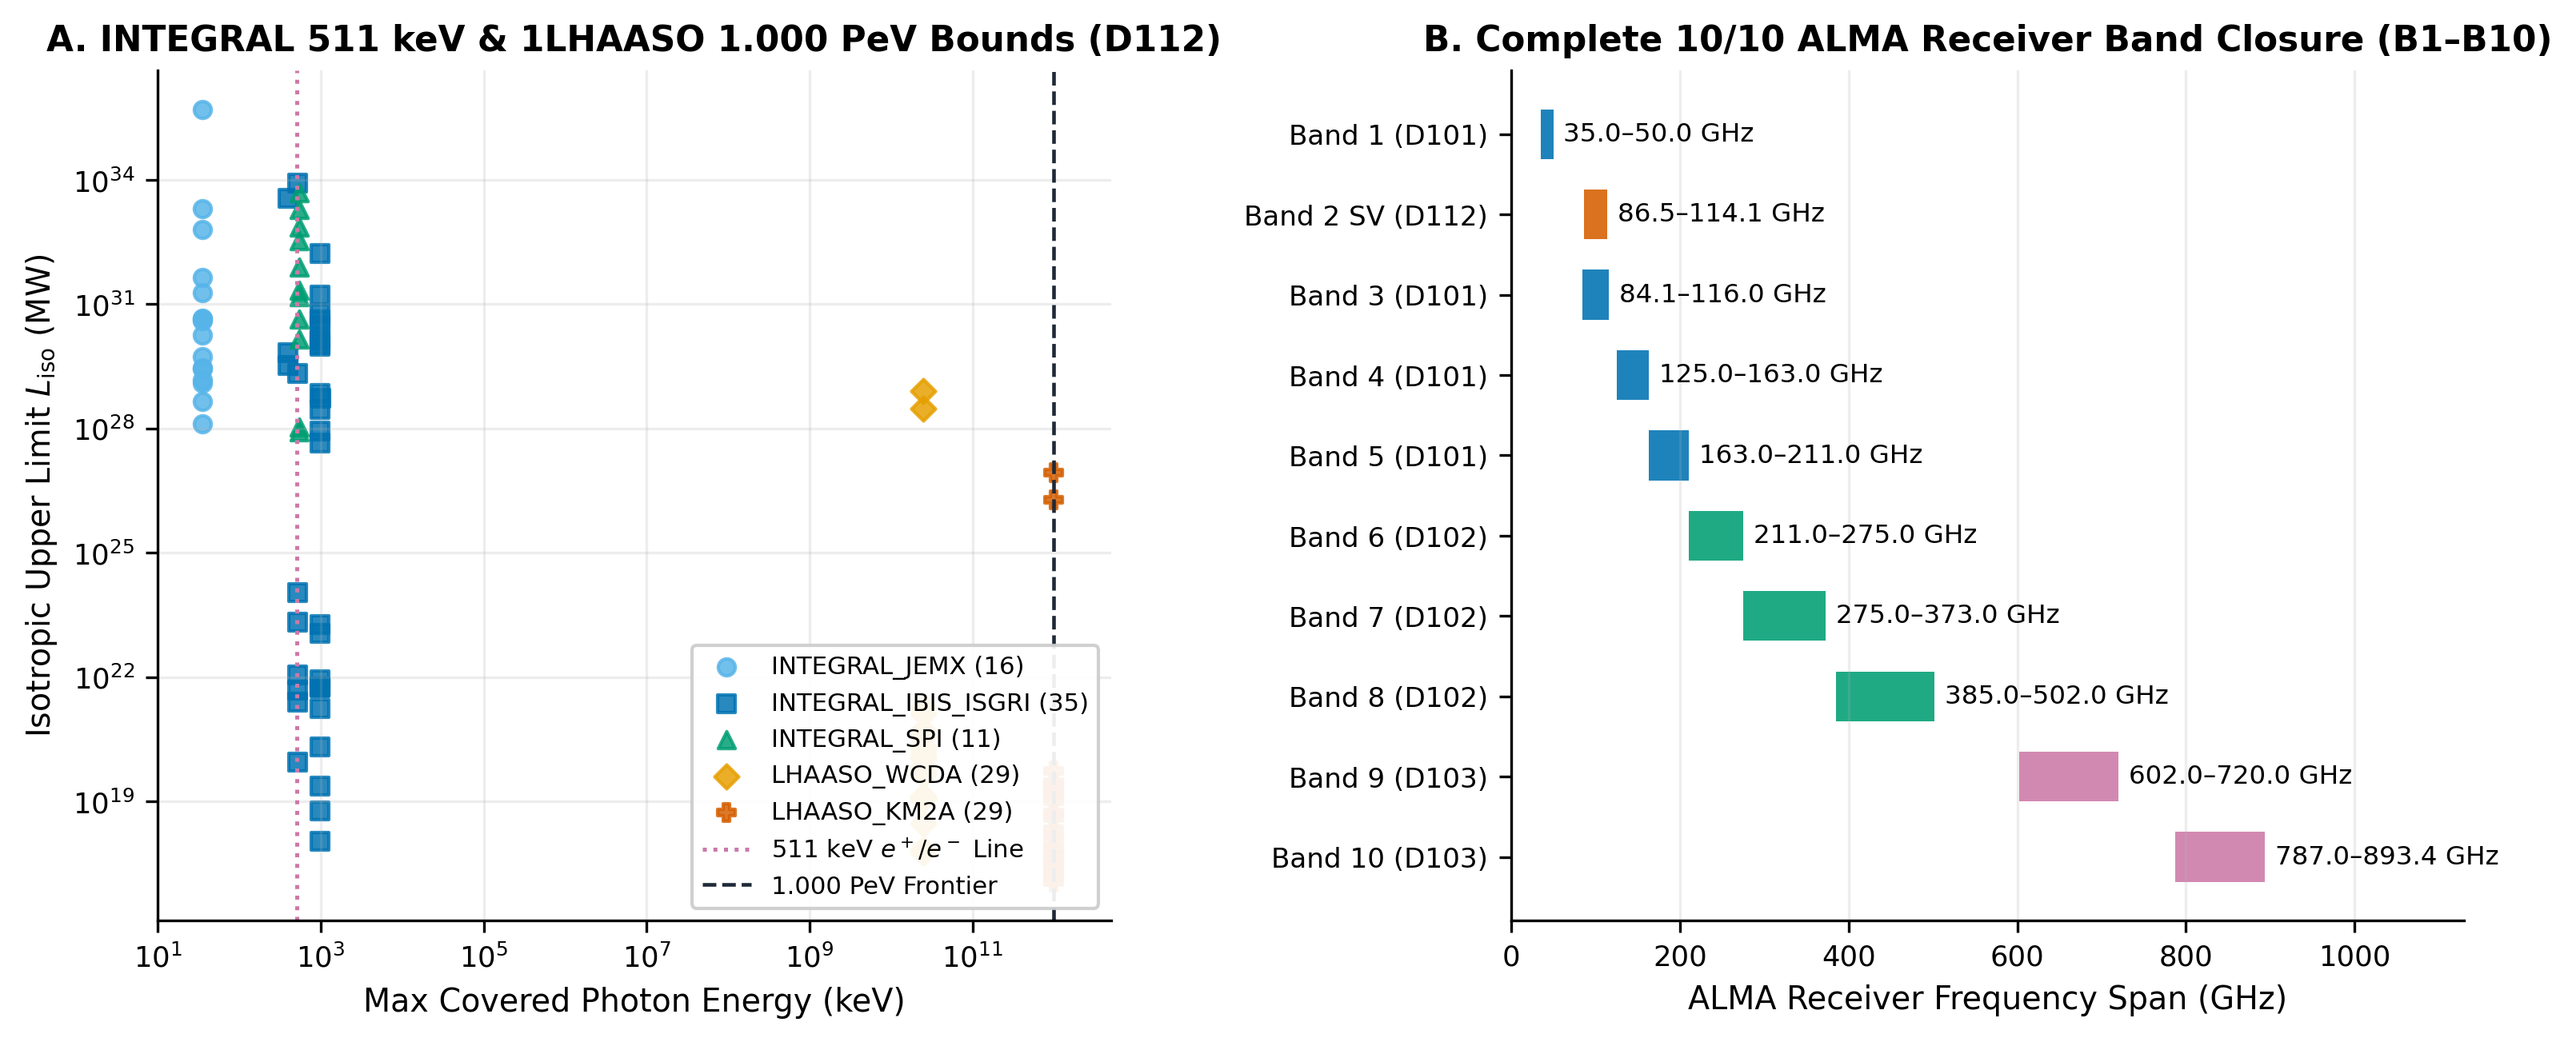
\includegraphics[width=0.95\textwidth]{figures/figJ07_high_energy_pev_511kev_and_alma_10of10.png}
\caption{\textbf{High-energy PeV/511\,keV frontier and complete 10/10 \textit{ALMA} closure.} \textbf{A:} $6\sigma$ isotropic luminosity bounds across $62$ \textit{INTEGRAL} (\texttt{JEM-X}, \texttt{IBIS/ISGRI}, \texttt{SPI}) spectra bracketing $511\,\mathrm{keV}$ and $58$ \textit{1LHAASO} (\texttt{WCDA}+\texttt{KM2A}) tracks up to \textbf{1.000\,PeV} (\texttt{D112}, \textbf{0 ETI}). \textbf{B:} Complete \textbf{10/10 \textit{ALMA} receiver band coverage (\texttt{B1--B10})} spanning $35.0\text{--}893.4\,\mathrm{GHz}$ ($335.58\text{--}8{,}556.42\,\mu\text{m}$), closed by Band~2 SV cubes (\texttt{2011.0.00026.SV}).}
\label{fig:figJ07}
\end{figure*}

% =========================================================================
\section{1,083-Star Scale-Separated Synthesis and \texttt{<10 pc} Volume Census}
\label{sec:synthesis}
% =========================================================================

\begin{figure*}[t]
\centering
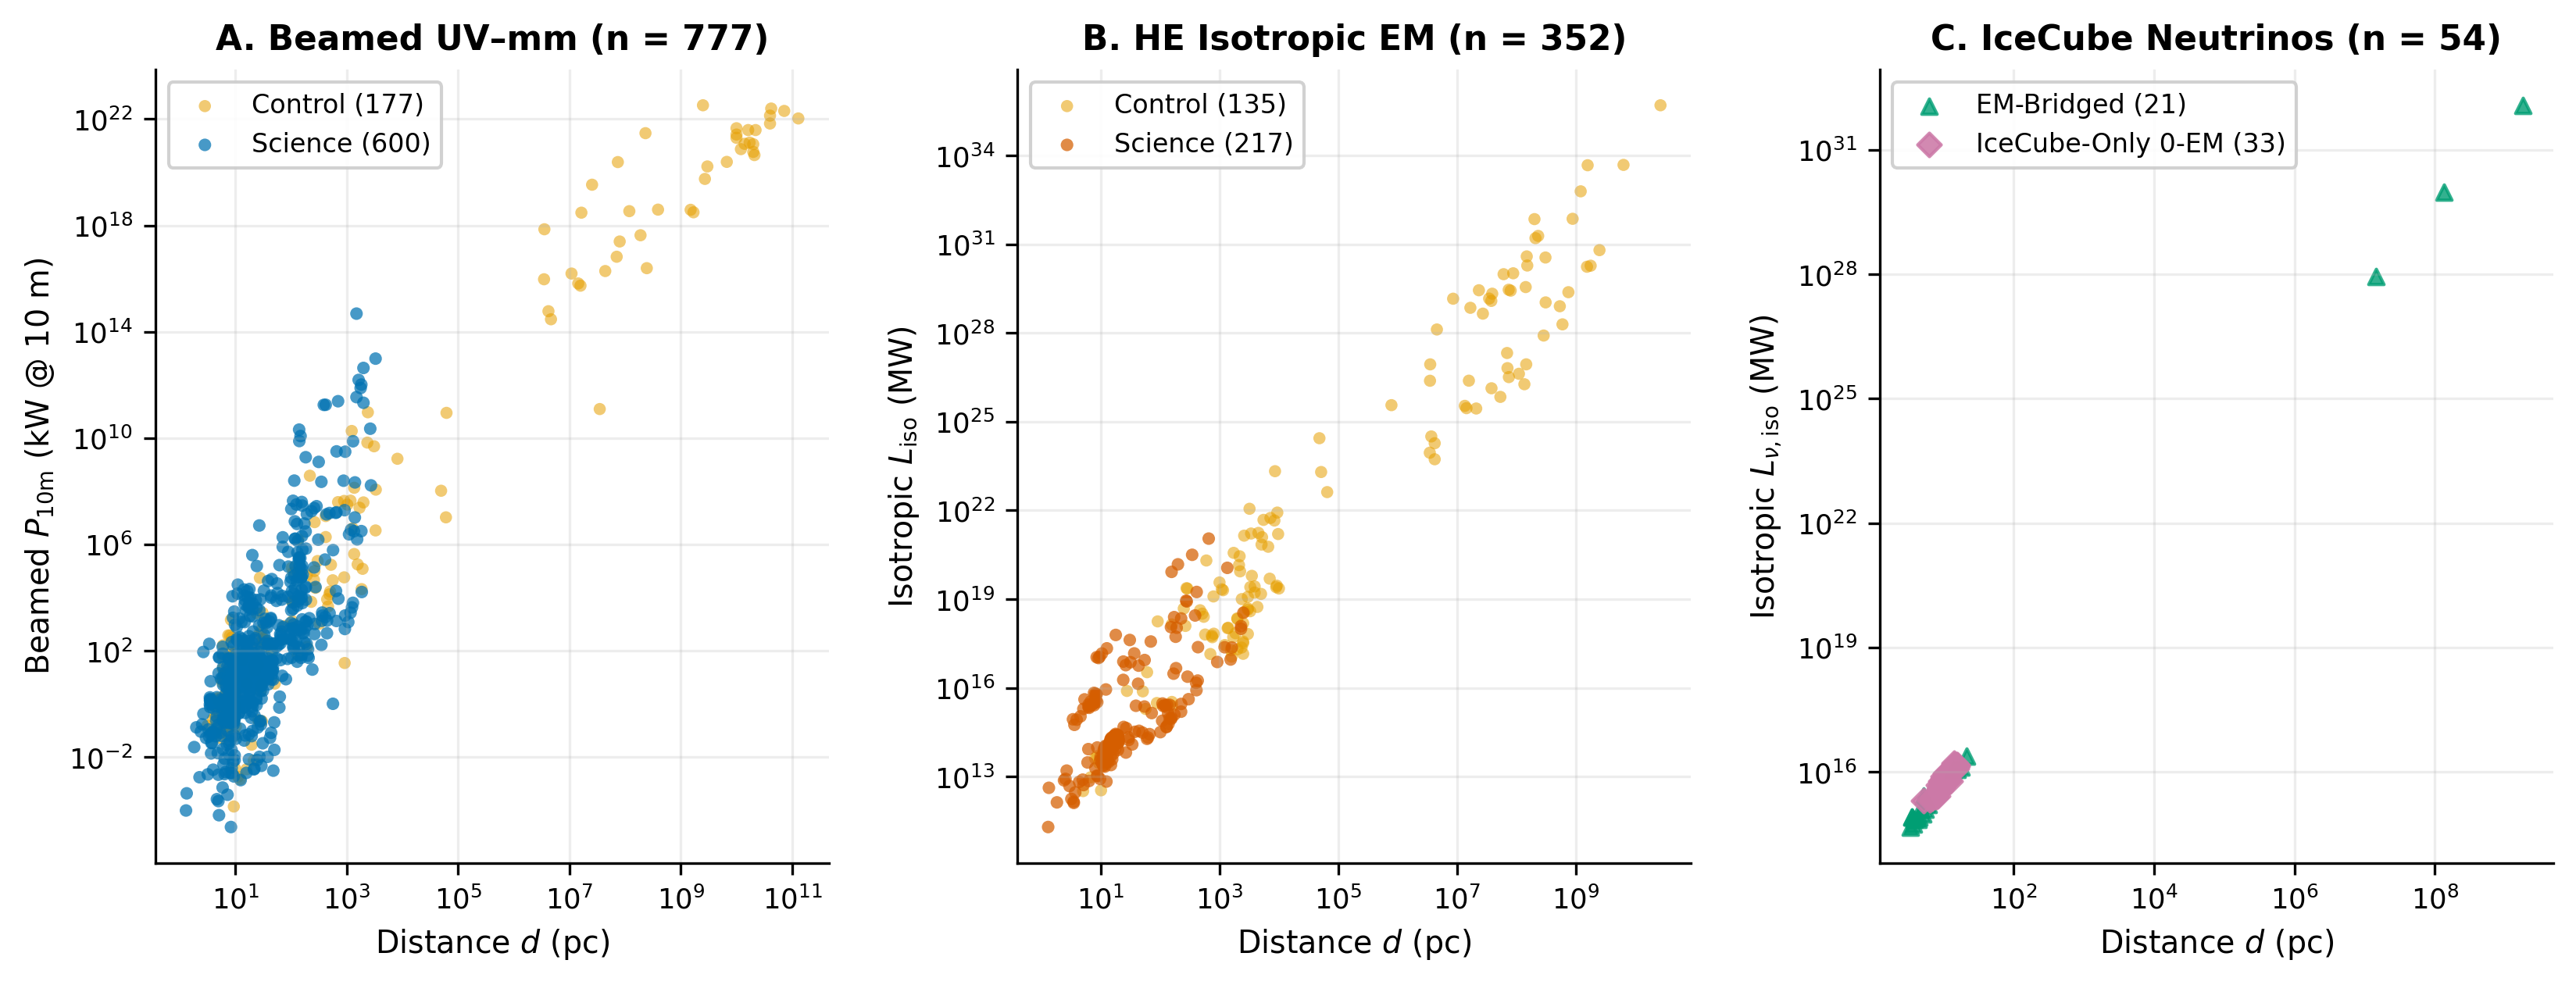
\includegraphics[width=0.96\textwidth]{figures/figJ04_three_regime_physical_scale_separation_1083stars.png}
\caption{\textbf{Strict three-regime physical scale separation across 1,083 targets (\texttt{table1}).} \textbf{A:} Diffraction-beamed $D_{\mathrm{tx}}=10\,\mathrm{m}$ laser/mm limits ($n=777$: $600$ Science + $177$ Control, $0.0905\text{--}8{,}556.42\,\mu\text{m}$). \textbf{B:} High-energy isotropic EM luminosity limits ($n=352$: $217$ Science + $135$ Control, EUV to $1.000\,\mathrm{PeV}$), kept strictly separate from optical $10\,\mathrm{m}$ beaming. \textbf{C:} \textit{IceCube} $\nu_\mu$ isotropic bounds ($n=54$: $21$ EM-bridged + \textbf{33 strictly \textit{IceCube}-only zero-EM stars} with blank EM cells preserved).}
\label{fig:figJ04}
\end{figure*}

A central methodological pillar of our synthesis (\texttt{D109--D112}) is \textbf{strict three-regime physical scale separation} (Figure~\ref{fig:figJ04}; machine-readable \texttt{table1} and \texttt{table4}):
\begin{enumerate}
  \item \textbf{Diffraction-Beamed UV--mm ($n=777$ targets: $600$ Science + $177$ Control):} Evaluated at a canonical transmitter aperture $D_{\mathrm{tx}}=10\,\mathrm{m}$, where $P_{10\mathrm{m}}$ scales quadratically with distance and $\lambda^2$. Across our volume-limited \textbf{267-star $<10\,\mathrm{pc}$ sample} (\texttt{table2}: $212$ Science [$61$ hosts / $121$ exoplanets] + $55$ Controls; Figure~\ref{fig:figJ02}A), the median beamed UV--mm threshold is \textbf{0.78810\,kW} ($0.829\,\mathrm{kW}$ in optical/IR alone), reaching sub-watt sensitivity on nearby degenerates and M dwarfs (\texttt{WD\,1334-039} \textbf{23.21\,mW}, \texttt{GJ\,1116\,B} \textbf{64.6\,mW}, \texttt{Proxima Cen} \textbf{97.3\,mW}, \texttt{WD\,0435-088} \textbf{137.4\,mW}, \texttt{GJ\,832} \textbf{219.4\,mW}, \texttt{GJ\,876} \textbf{259.1\,mW}).
  \item \textbf{High-Energy Isotropic EM ($n=352$ targets: $217$ Science + $135$ Control):} EUV, X-ray, MeV/GeV, VHE TeV, and PeV limits are reported strictly in physical photon flux $F_{\mathrm{lim}}$ ($\mathrm{erg\,cm^{-2}\,s^{-1}}$) and isotropic luminosity $L_{\mathrm{iso}} = 4\pi d^2 F_{\mathrm{lim}}$ ($\mathrm{MW}$) without mixing diffraction gain into optical medians. Deepest HE bounds reach $1.956\times 10^{11}\,\mathrm{MW}$ (\texttt{Proxima Cen}, \textit{XMM RGS}), $1.279\times 10^{12}\,\mathrm{MW}$ (\texttt{Procyon}), $1.334\times 10^{12}\,\mathrm{MW}$ (\texttt{Barnard's Star}, \textit{Swift XRT}), $1.408\times 10^{12}\,\mathrm{MW}$ (\texttt{61\,Cyg\,B}, \textit{Chandra LETG}), and $1.744\times 10^{12}\,\mathrm{MW}$ ($\epsilon$\,\texttt{Eri}).
  \item \textbf{Isotropic Neutrino Multi-Messenger ($n=54$ targets; $33$ \textit{IceCube}-Only Zero-EM):} Neutrino flux and luminosity bounds ($L_{\nu,\mathrm{iso}}$, down to $4.676\times 10^{14}\,\mathrm{MW}$ on \texttt{Ross\,128}) never populate EM summary columns; all $33$ \textit{IceCube}-only targets and $126/126$ \textit{IceCube} rows in \texttt{table4} retain explicit null (\texttt{---}) EM values.
\end{enumerate}

Table~\ref{tab:records} highlights representative flagship constraints across regimes, and Figure~\ref{fig:figJ02}B illustrates our \textbf{197 Science bridge systems} ($262$ multi-phase targets spanning $2{,}695$ calibrated bridge cells), topped by \texttt{AU\,Mic} ($16$ instruments from \textit{EUVE} and \textit{RXTE} to \textit{ALMA} B3/B6), $\epsilon$\,\texttt{Eri} ($14$ instruments), \texttt{Proxima Cen} ($10$), \texttt{Eta Carinae} ($10$), \texttt{tau Cet} ($9$), \texttt{3C\,273} ($9$), \texttt{Betelgeuse} ($9$), and \texttt{Cen\,A} ($9$).

\begin{figure*}[t]
\centering
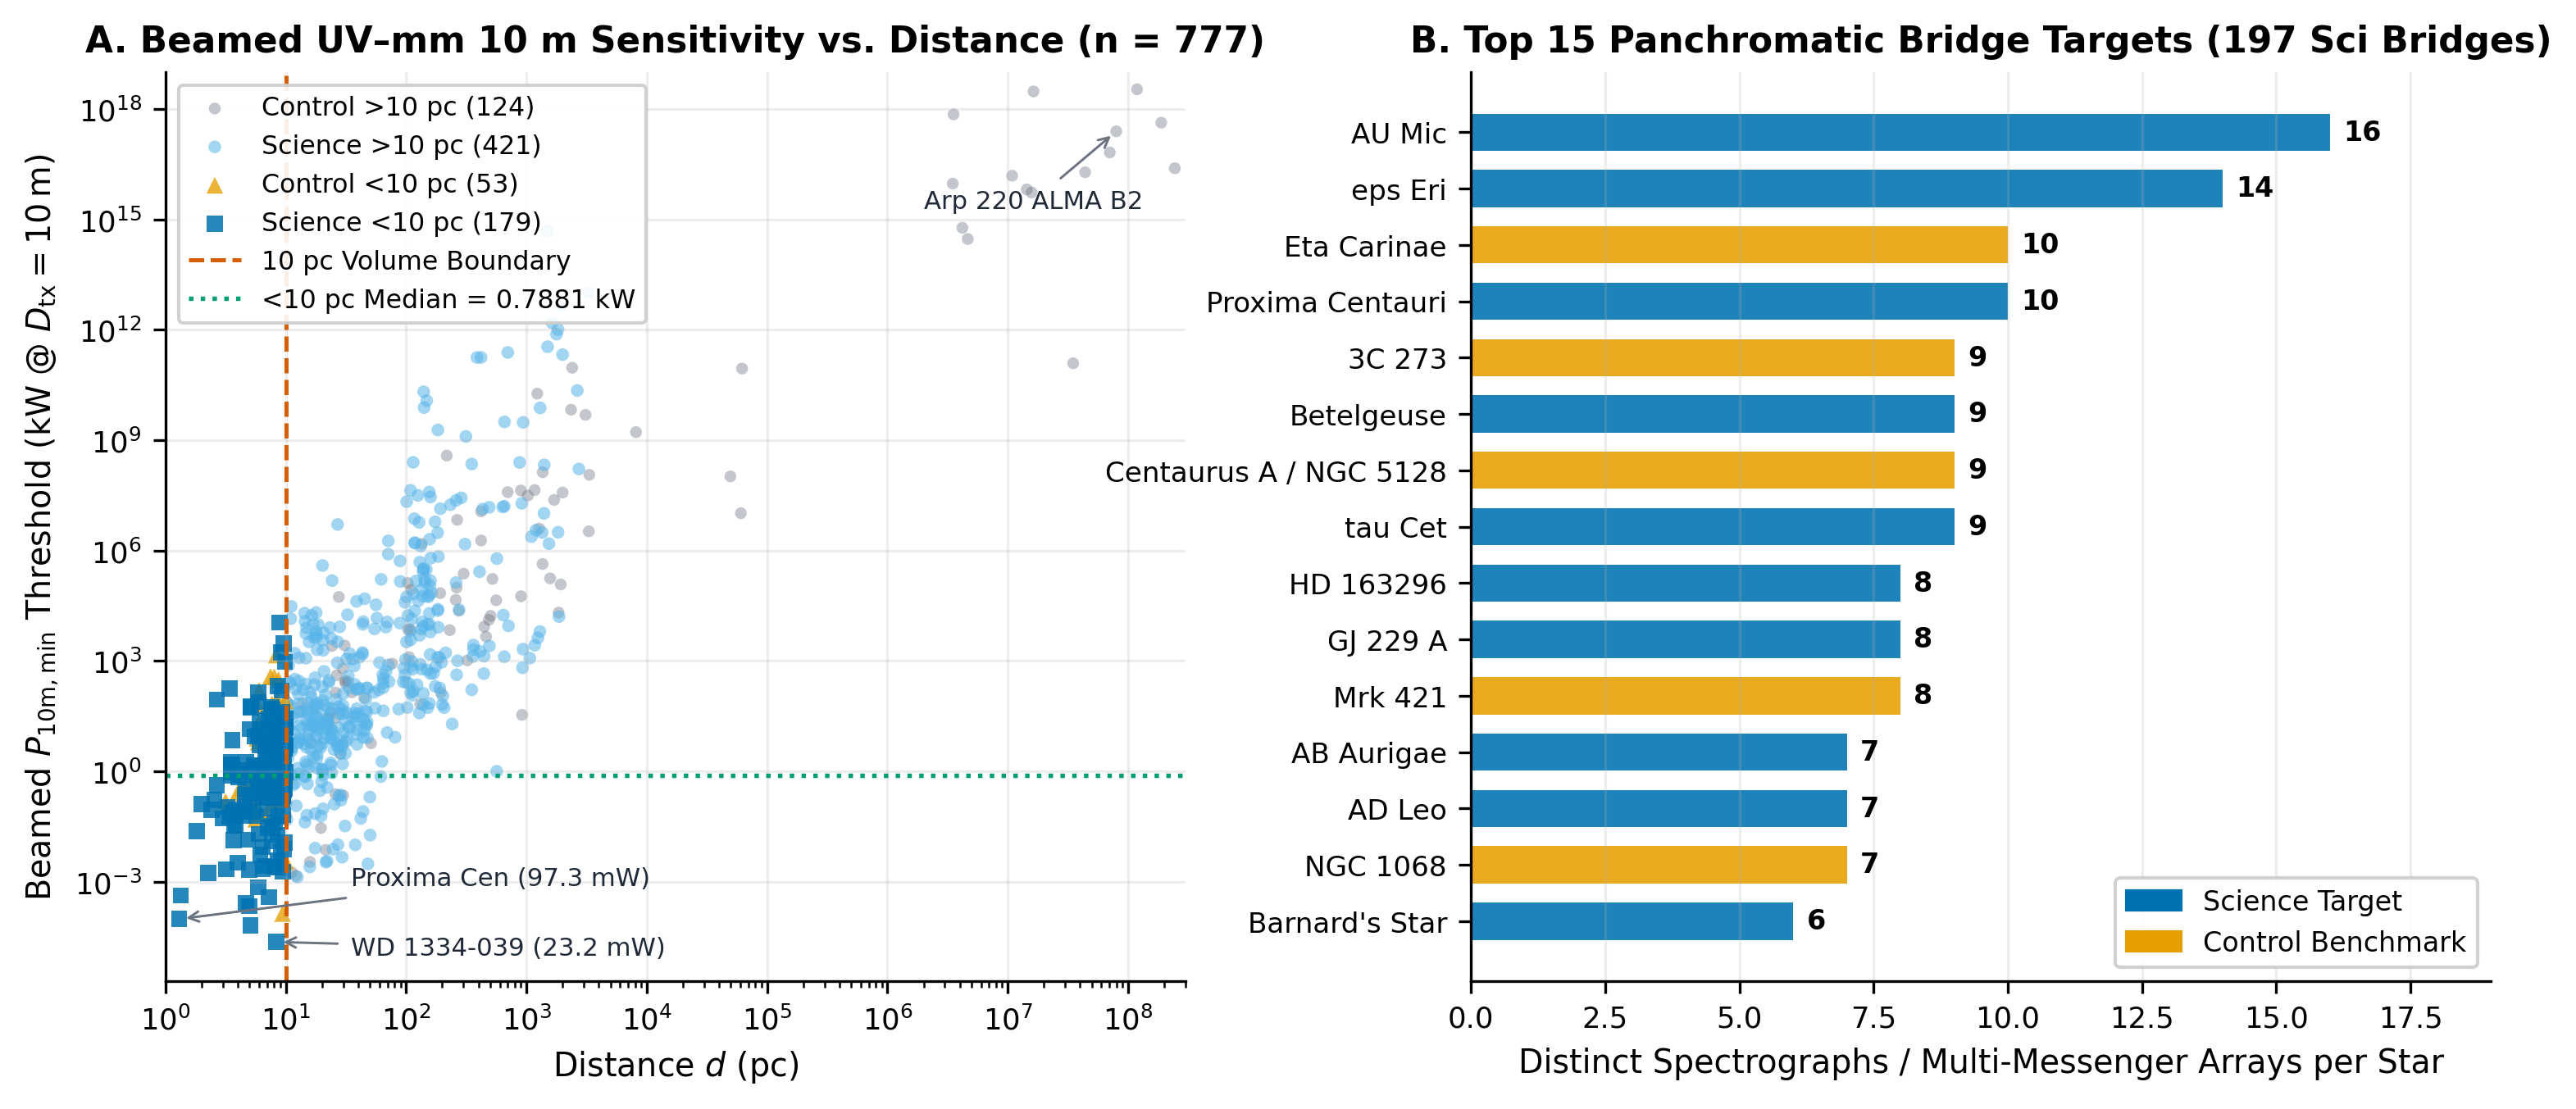
\includegraphics[width=0.95\textwidth]{figures/figJ02_solar_neighborhood_10pc_and_bridge_census.png}
\caption{\textbf{Volume-limited $<10\,\mathrm{pc}$ sensitivity and multi-instrument bridges.} \textbf{A:} Distance vs.\ $10\,\mathrm{m}$ beamed UV--mm upper limit ($n=777$), highlighting the \textbf{267-star $<10\,\mathrm{pc}$ census} ($0.7881\,\mathrm{kW}$ median; down to $23.2\,\mathrm{mW}$ on \texttt{WD\,1334-039} and $97.3\,\mathrm{mW}$ on \texttt{Proxima Cen}). \textbf{B:} Top $15$ multi-phase panchromatic bridge targets (\texttt{table4}, $2{,}695$ total cells), led by \texttt{AU\,Mic} ($16$ instruments) and $\epsilon$\,\texttt{Eri} ($14$).}
\label{fig:figJ02}
\end{figure*}

\begin{table*}[t]
\centering
\caption{Selected Deepest Physical Technosignature Upper Limits Across Wavelength, Polarization, and Neutrino Regimes (\texttt{0 Verified ETI}).}
\label{tab:records}
\resizebox{\textwidth}{!}{%
\begin{tabular}{llclllr}
\toprule
Regime & Target (Role) & Dist.\ (pc) & Instrument / Arm & Spectral / Energy Window & Tightest Physical Bound & Archive \\
\midrule
Beamed Opt. & \texttt{WD\,1334-039} (Sci) & 8.35 & \texttt{ESO\_UVES} & $0.48\text{--}1.04\,\mu\text{m}$ & $P_{10\mathrm{m}} = \mathbf{23.21\,\mathrm{mW}}$ & \texttt{AF} \\
Beamed FUV & \texttt{Proxima Cen} (Sci) & 1.302 & \texttt{HST\_STIS} & $0.1145\text{--}0.171\,\mu\text{m}$ & $P_{10\mathrm{m}} = \mathbf{97.30\,\mathrm{mW}}$ & \texttt{M} \\
Beamed Opt. Ctrl & \texttt{WD\,0435-088} (Ctrl) & 9.40 & \texttt{ESO\_UVES} & $0.48\text{--}1.04\,\mu\text{m}$ & $P_{10\mathrm{m}} = \mathbf{137.4\,\mathrm{mW}}$ & \texttt{AH} \\
Beamed Opt.-Pol & \texttt{GJ\,729} (Sci) & 2.98 & \texttt{CFHT\_ESPADONS\_POL} & $0.37\text{--}1.05\,\mu\text{m}$ ($V$) & $P_{10\mathrm{m}} = \mathbf{52.19\,\mathrm{W}}$ ($\mathrm{MDP}_{99}\,0.41\%$) & \texttt{AJ} \\
Beamed NIR-Pol & \texttt{Wolf\,359} (Sci) & 2.41 & \texttt{CFHT\_SPIROU\_POL} & $0.96\text{--}2.52\,\mu\text{m}$ ($V$) & $P_{10\mathrm{m}} = \mathbf{90.28\,\mathrm{W}}$ & \texttt{AJ} \\
Beamed QCL IR & \texttt{WISE\,0855} (Sci) & 2.28 & \texttt{JWST\_NIRSPEC\_G395M} & $3.1\,\mu\text{m}$ $L$-band & $P_{10\mathrm{m}} = \mathbf{1.733\,\mathrm{W}}$ & \texttt{AK} \\
ALMA Band~2 SV & \texttt{Arp\,220} (Ctrl) & $7.7\times 10^7$ & \texttt{ALMA\_B2\_3MM} (\texttt{X52}) & $86.45\text{--}114.12\,\mathrm{GHz}$ & $P_{10\mathrm{m}} = 2.487\times 10^{17}\,\mathrm{kW}$ ($10/10$ bands) & \texttt{AL} \\
Soft X-Ray Iso. & \texttt{Proxima Cen} (Sci) & 1.302 & \texttt{XMM\_RGS} & $0.33\text{--}2.48\,\mathrm{keV}$ & $L_{\mathrm{iso}} = \mathbf{1.956\times 10^{11}\,\mathrm{MW}}$ & \texttt{AC} \\
511\,keV / Hard-X & \texttt{SS\,Cyg} (Ctrl) & 112.9 & \texttt{INTEGRAL\_IBIS\_ISGRI} & $13\text{--}970.9\,\mathrm{keV}$ & $L_{\mathrm{iso}} = 1.073\times 10^{18}\,\mathrm{MW}$ ($F_{\mathrm{lim}}\,7.03\times 10^{-12}$) & \texttt{AL} \\
PeV Gamma Iso. & \texttt{J0622+3754} (Ctrl) & $1.6\times 10^3$ & \texttt{LHAASO\_KM2A} & $25\text{--}\mathbf{1{,}000\,\mathrm{TeV}}$ ($1\,\mathrm{PeV}$) & $L_{\mathrm{iso}} = 1.136\times 10^{17}\,\mathrm{MW}$ & \texttt{AL} \\
Neutrino Iso. & \texttt{Ross\,128} (Sci) & 3.37 & \texttt{ICECUBE\_10YR} & $0.1\,\mathrm{TeV}\text{--}10\,\mathrm{PeV}$ $\nu_\mu$ & $L_{\nu,\mathrm{iso}} = \mathbf{4.676\times 10^{14}\,\mathrm{MW}}$ & \texttt{AG} \\
\bottomrule
\end{tabular}%
}
\end{table*}

% =========================================================================
\section{Bayesian Occurrence Bounds ($f_{\mathrm{tx}}$) and Haystack Benchmarks}
\label{sec:bayesian}
% =========================================================================

With $k = 0$ verified detections across $N_{\mathrm{eff}} = \sum_{i=1}^{N_{\mathrm{sens}}} c_{\mathrm{cal}}\,[1 - (1 - \eta)^{n_{\mathrm{nights},i}}]$ completeness-weighted and duty-cycle-weighted targets ($\eta \in \{1.0, 0.5, 0.1, 0.01\}$; multi-epoch revisit gain explicitly increases $N_{\mathrm{eff}}$ when $\eta < 1$), the 95\% credible upper bound on transmitter prevalence $f_{\mathrm{tx}}$ is obtained from the binomial posterior under both a conservative Uniform($0,1$) prior ($f_{95,\mathrm{U}} = 1 - 0.05^{1/(N_{\mathrm{eff}}+1)}$) and the exact uninformative Jeffreys $\mathrm{Beta}(0.5, N_{\mathrm{eff}}+0.5)$ quantile ($f_{95,\mathrm{J}}$ evaluated via inverse regularized incomplete Beta function), alongside frequentist Clopper--Pearson bounds (\texttt{table5}).

\begin{table*}[t]
\centering
\caption{Bayesian and Frequentist 95\% Upper Limits on Transmitter Occurrence Rate ($f_{95}$, Steady $\eta=1.0$ vs.\ Pulsed/Duty-Cycled $\eta=0.1$) from \texttt{table5}.}
\label{tab:bayesian}
\resizebox{\textwidth}{!}{%
\begin{tabular}{llrrrrrrr}
\toprule
Regime & Cohort & Threshold & $n_{\mathrm{sens}}$ & $N_{\mathrm{eff}}$ ($\eta=1$) & $f_{95,\mathrm{U}}$ ($\eta=1$) & $f_{95,\mathrm{J}}$ Exact Beta & $f_{95,\mathrm{CP}}$ ($\eta=1$) & $f_{95,\mathrm{U}}$ ($\eta=0.1$) \\
\midrule
Beamed UV--mm & \texttt{ALL\_SCIENCE\_EM} & Any Calibrated & 600 & 591.00 & \textbf{0.5048\%} & \textbf{0.3243\%} & 0.5056\% & 1.5594\% \\
Beamed UV--mm & \texttt{ALL\_SCIENCE\_EM} & $P_{10\mathrm{m}}\le 10\,\mathrm{kW}$ & 250 & 246.25 & 1.2044\% & 0.7755\% & 1.2092\% & 2.9125\% \\
Beamed UV--mm & \texttt{ALL\_SCIENCE\_EM} & $P_{10\mathrm{m}}\le 1\,\mathrm{kW}$ & 146 & 143.81 & 2.0472\% & 1.3233\% & 2.0616\% & 4.9964\% \\
Beamed UV--mm & \texttt{EXOPLANET\_HOSTS} & Any Calibrated & 298 & 293.53 & \textbf{1.0120\%} & \textbf{0.6517\%} & 1.0154\% & 2.3946\% \\
Beamed UV--mm & \texttt{SOLAR\_10PC\_SCI} & Any Calibrated & 179 & 176.32 & \textbf{1.6753\%} & \textbf{1.0819\%} & 1.6847\% & 4.0879\% \\
Beamed UV--mm & \texttt{SOLAR\_10PC\_SCI} & $P_{10\mathrm{m}}\le 10\,\mathrm{kW}$ & 153 & 150.71 & 1.9546\% & 1.2631\% & 1.9675\% & 4.6050\% \\
HE Isotropic & \texttt{ALL\_HE\_ISOTROPIC\_EM} & Any Calibrated & 352 & 350.59 & \textbf{0.8484\%} & \textbf{0.5460\%} & 0.8508\% & 3.9673\% \\
HE Isotropic & \texttt{EXOPH\_HE\_EM} & Any Calibrated & 217 & 215.26 & 1.3757\% & 0.8873\% & 1.3820\% & 6.1854\% \\
Neutrino Iso. & \texttt{ICECUBE\_NEUTRINO} & Any Calibrated & 54 & 53.35 & \textbf{5.3626\%} & \textbf{3.5198\%} & 5.4603\% & 37.6793\% \\
\bottomrule
\end{tabular}%
}
\end{table*}

Table~\ref{tab:bayesian} and Figure~\ref{fig:figJ08} summarize these constraints. Notice that our multi-epoch revisit depth (up to $31$ distinct nights on \texttt{Proxima Cen}) prevents linear collapse when $\eta=0.1$: for \texttt{ALL\_SCIENCE\_EM}, $f_{95,\mathrm{U}}$ tightens from $4.44\%$ ($P_{10\mathrm{m}}\le 0.1\,\mathrm{kW}$) to \textbf{0.5048\%} (\textbf{0.3243\%} Jeffreys) across all $n=600$ Science EM targets, and stays at $1.5594\%$ even for a $10\%$ duty cycle. Compared against landmark narrow-band searches via the Continuous Waveform Transmitter Figure of Merit ($\mathrm{CWTFM} = \mathrm{EIRP}_{\mathrm{med}} / [N_\star \nu_{\mathrm{rel}}]$;~\cite{Enriquez2017,Wright2018}), Tellis \& Marcy~\cite{TellisMarcy2017} reach $f_{95} = 0.0535\%$ across $5{,}600$ optical stars ($\Delta\log_2\nu = 1.116$ octaves) and Price et al.~\cite{Price2020} reach $0.2253\%$ across $1{,}327$ $L/S$-band radio stars ($1.40$ octaves), whereas our survey trades extreme single-band star count for an order-of-magnitude expansion in electromagnetic octave breadth (\textbf{62.582 octaves}, $\nu_{\mathrm{rel}} = 44.70$; $45.682$ HE octaves + $14.693$ Lyman-to-\texttt{B4} octaves + \textit{IceCube} neutrinos + Stokes polarimetry; Figure~\ref{fig:figJ08}B).

\begin{figure*}[t]
\centering
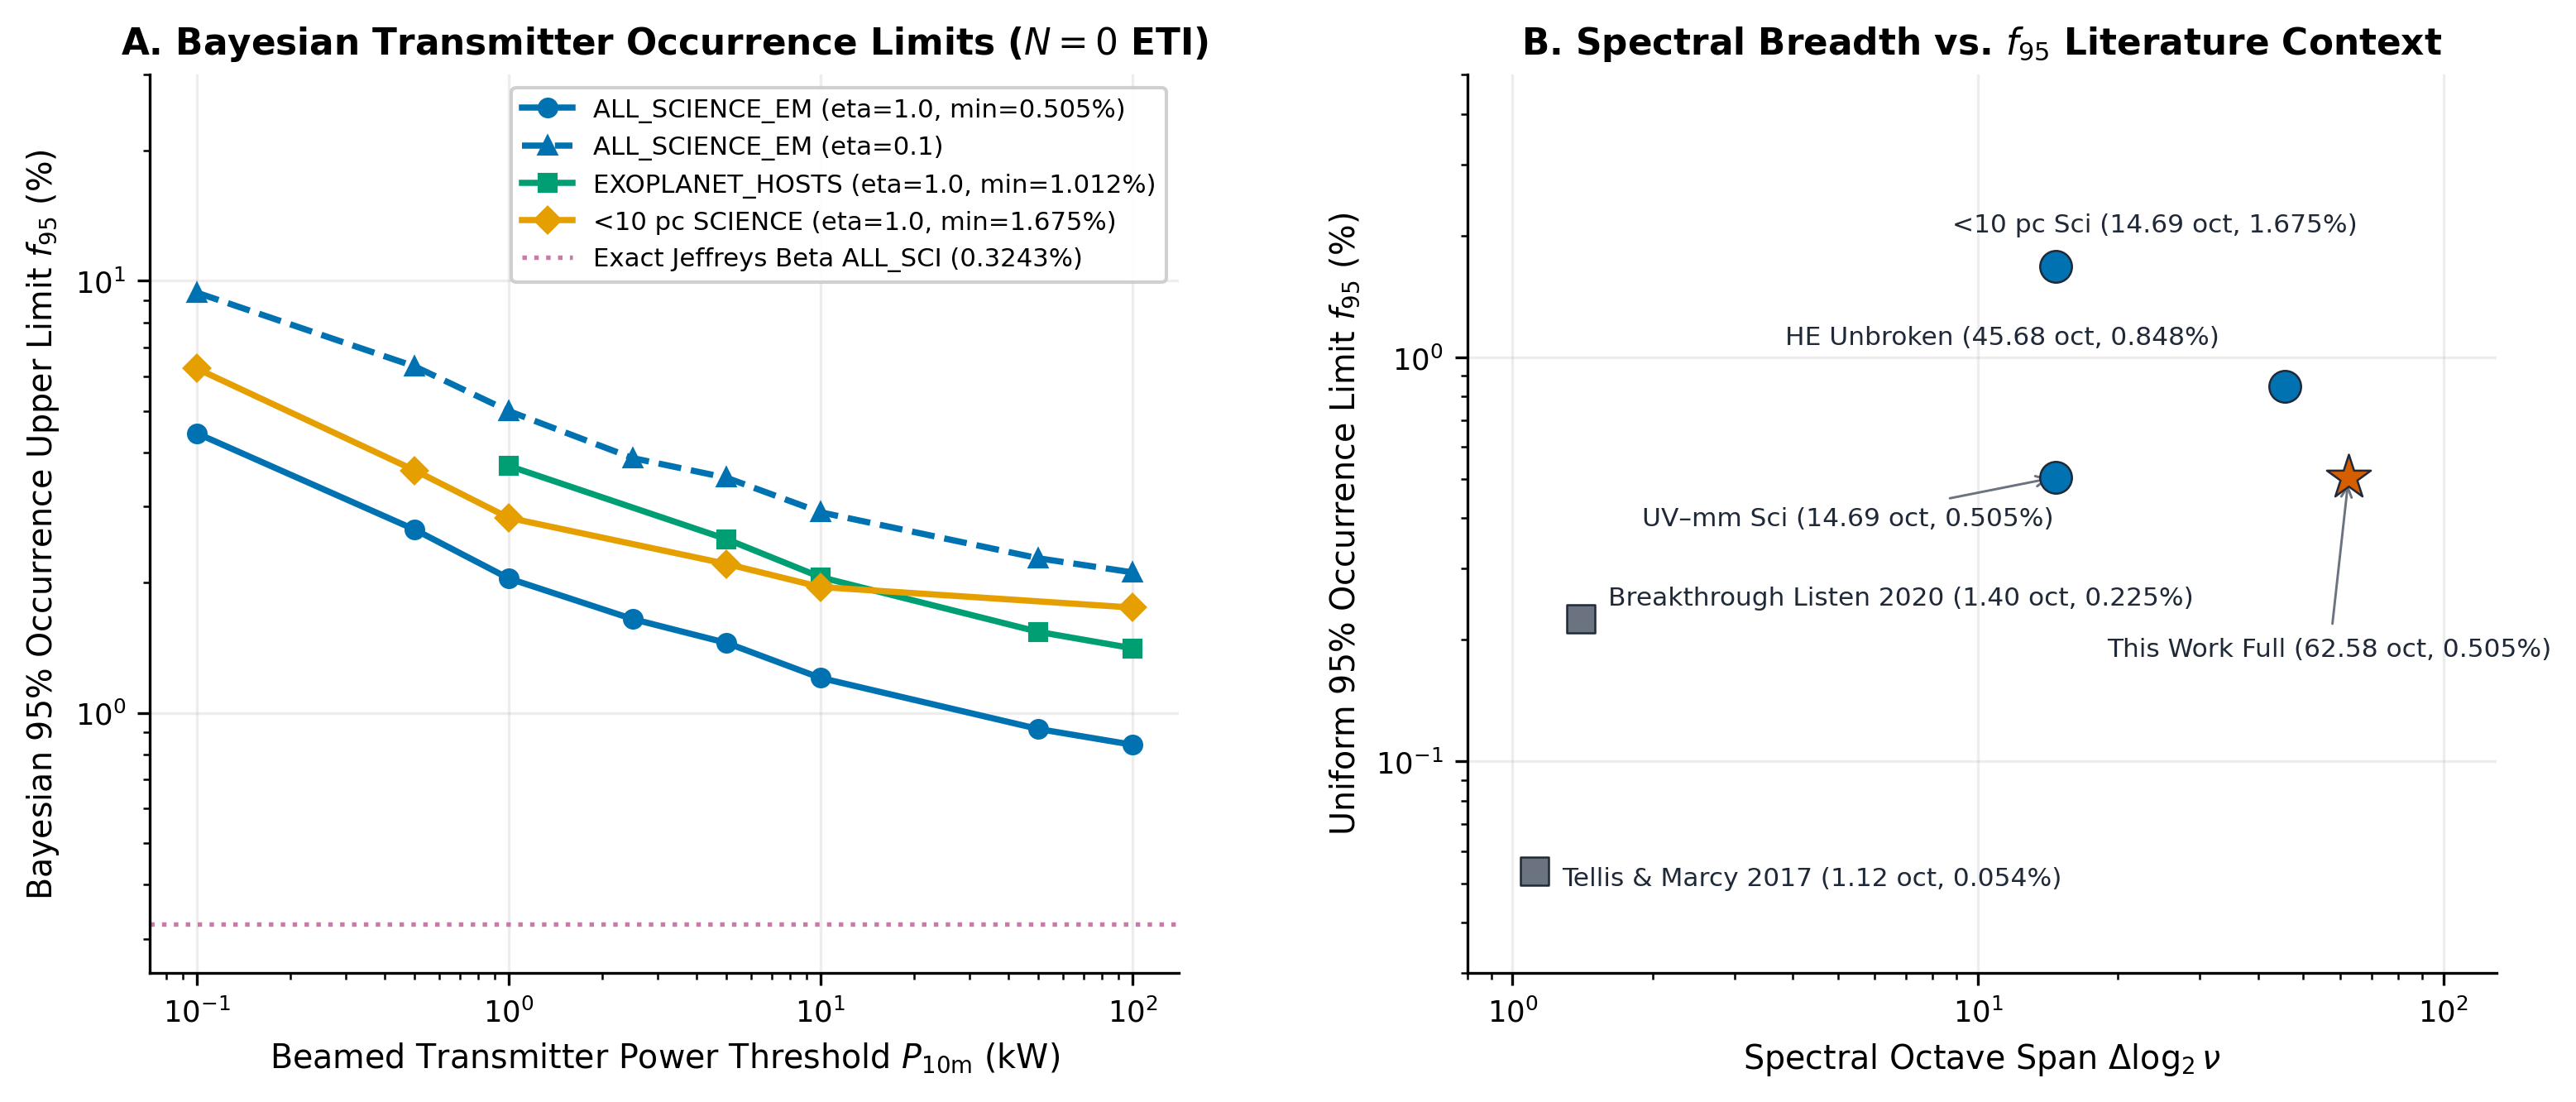
\includegraphics[width=0.95\textwidth]{figures/figJ08_bayesian_ftx_and_cosmic_haystack_cwtfm.png}
\caption{\textbf{Bayesian occurrence bounds and Cosmic Haystack literature comparison.} \textbf{A:} Uniform 95\% upper bounds $f_{95}$ (\texttt{table5}) as a function of beamed threshold $P_{10\mathrm{m}}$ for $\eta=1.0$ and $\eta=0.1$, compared to the exact $\mathrm{Beta}(0.5, N_{\mathrm{eff}}+0.5)$ Jeffreys baseline ($0.3243\%$ on \texttt{ALL\_SCIENCE\_EM}). \textbf{B:} Spectral octave breadth $\Delta\log_2\nu$ vs.\ $f_{95}$ against Tellis \& Marcy (2017)~\cite{TellisMarcy2017} and Breakthrough Listen (Price et al.\ 2020)~\cite{Price2020} (\texttt{table5b}).}
\label{fig:figJ08}
\end{figure*}

% =========================================================================
\section{Discussion: Methodological Gains, Limitations, and Future Directions}
\label{sec:discussion}
% =========================================================================
Five structural lessons emerge from completing thirty-four prospectively locked phases across \texttt{1,083} systems:
\begin{enumerate}
  \item \textit{Multi-Epoch Drift Closure Substantially Expands Kinematic Sensitivity:} Prior to Phase \texttt{D109}, only $8.2\%$ ($5/61$) of our $<10\,\mathrm{pc}$ planet hosts had been coherently searched against orbital Doppler accelerations; extending \texttt{DRIFT\_V67} to $61/61$ ($100.0\%$) demonstrated that no weak planetary-orbital beacon hides below our single-epoch detection limits across archived echelle epochs.
  \item \textit{Strict Physical Scale Decoupling Prevents False Optimism:} High-energy photon (EUV to $1\,\mathrm{PeV}$) and neutrino limits probe genuinely complementary astrophysics ($L_{\mathrm{iso}} \sim 10^{11}\text{--}10^{18}\,\mathrm{MW}$), and keeping them orthogonal to $10\,\mathrm{m}$ laser beaming yields clean, defensible population statistics.
  \item \textit{Residual Blind Spots Remaining After \texttt{D112}:} Even across $62.582$ octaves, two physical regions remain thinly sampled: (a) the $700\text{--}905\,\text{\AA}$ interstellar neutral-hydrogen absorption wall (fundamentally opaque beyond the Local Bubble) and atmospheric $\mathrm{O_2}/\mathrm{H_2O}$ telluric bands; and (b) centimeter-band ($1.4\text{--}35\,\mathrm{GHz}$) radio spectroscopy on the full $1{,}083$-star cohort beyond our $23/23$ Parkes/GBT overlap targets, together with sub-second pulsed optical/X-ray event-timing searches outside continuous spectroscopy.
  \item \textit{Extragalactic High-Luminosity Benchmarks:} Including \texttt{Arp\,220} (\textit{ALMA} Band~2 SV) and Fermi/TeV/INTEGRAL AGN controls constrains Kardashev Type~III-scale narrowband emission out to $z \approx 0.16$ while keeping Galactic $<10\,\mathrm{pc}$ star-forming statistics uncontaminated.
\end{enumerate}

% =========================================================================
\section{38-Archive Clean-Room Reproducibility and Independent Audit}
\label{sec:repro}
% =========================================================================

\begin{figure*}[t]
\centering
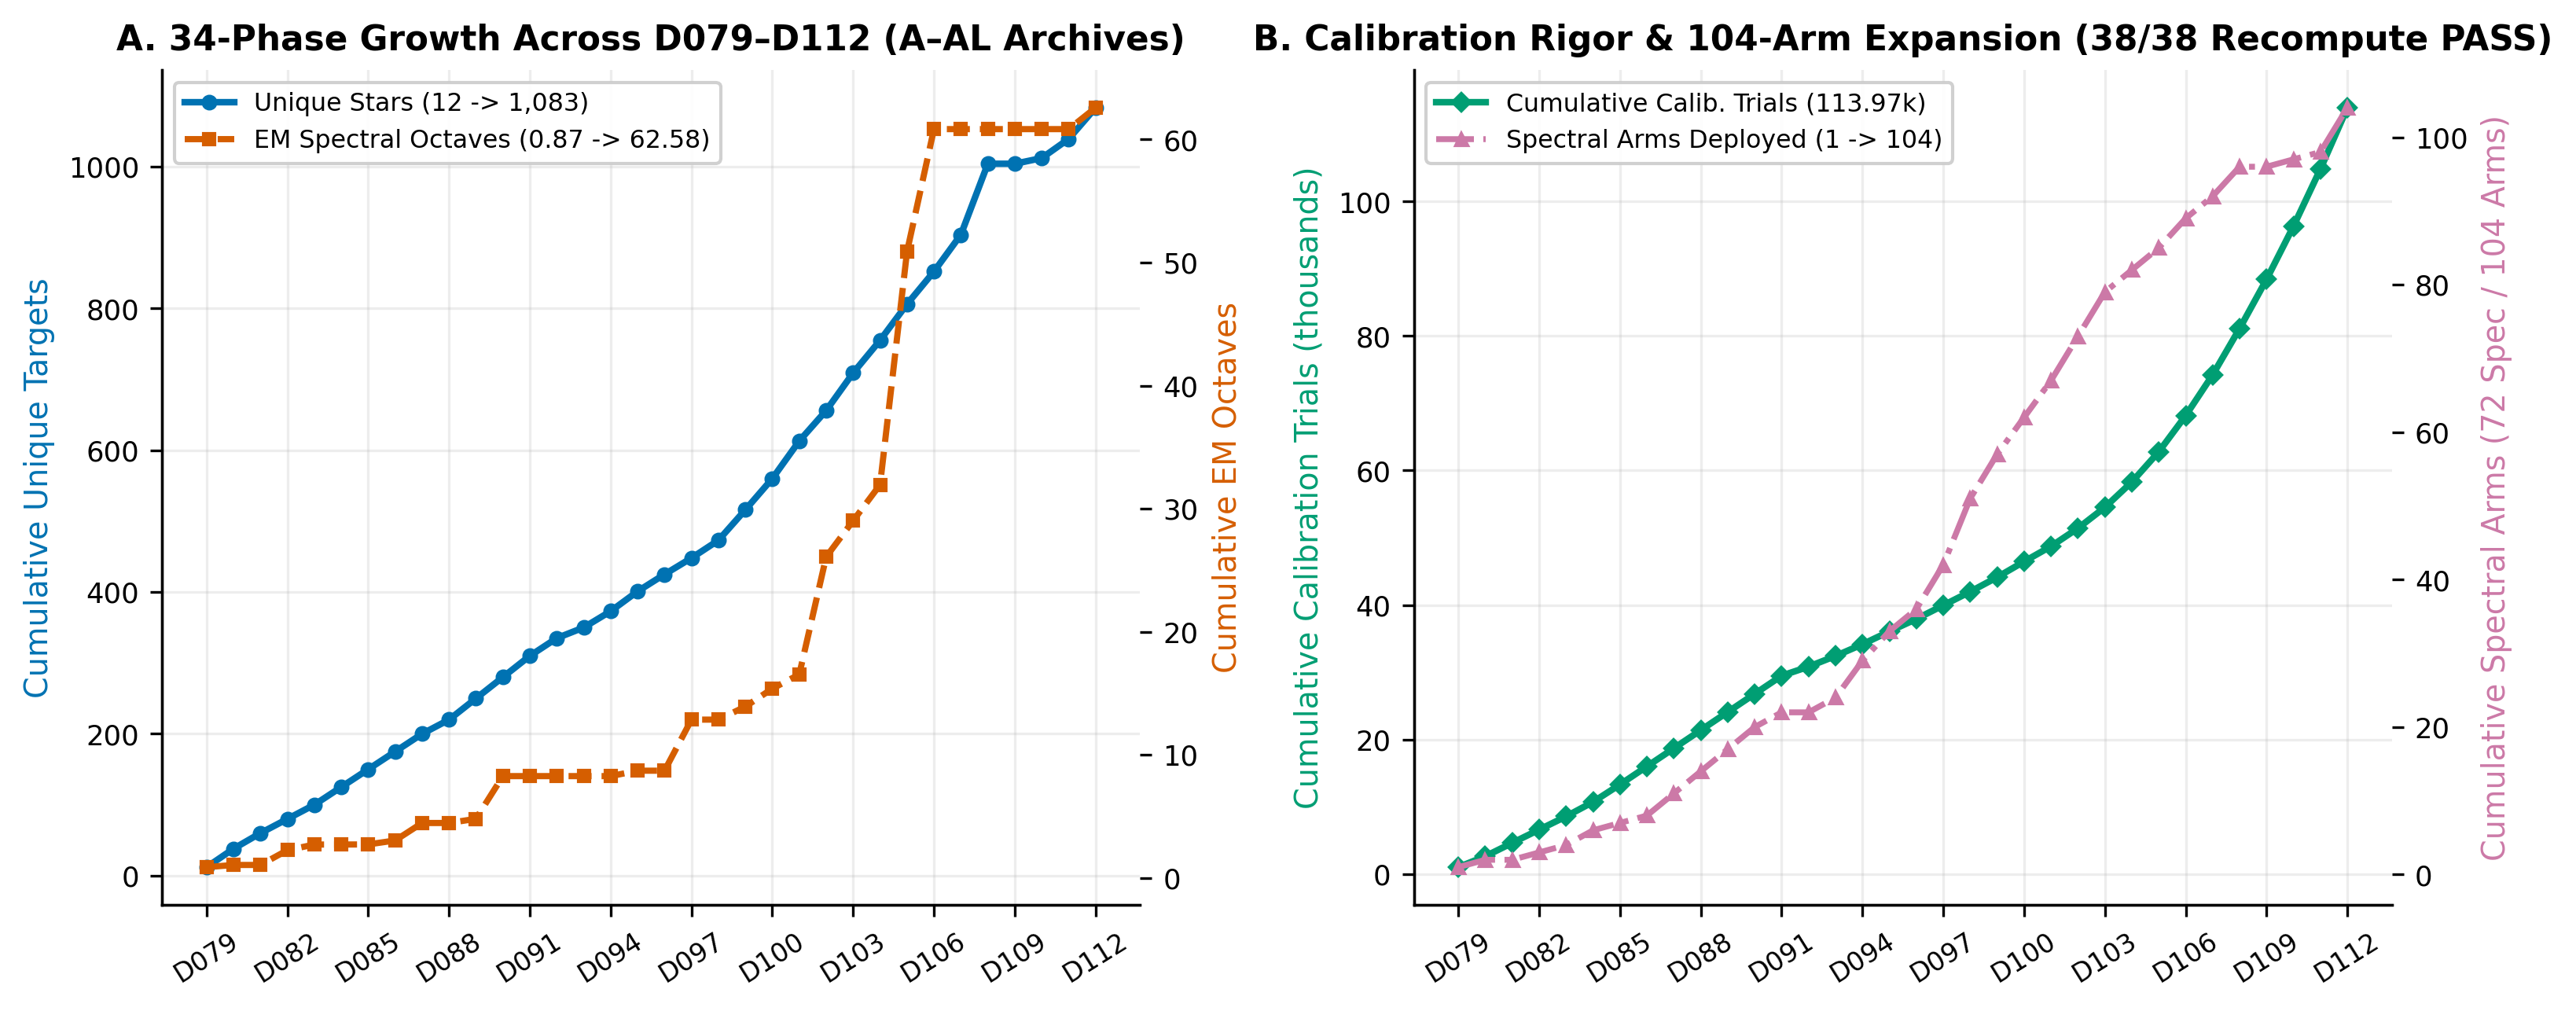
\includegraphics[width=0.95\textwidth]{figures/figJ09_survey_trajectory_and_reproducibility_chain.png}
\caption{\textbf{Thirty-four-phase survey trajectory and verification chain (\texttt{D079--D112}).} \textbf{A:} Cumulative expansion from $12 \rightarrow \mathbf{1{,}083}$ unique systems and $0.87 \rightarrow \mathbf{62.582}$ EM octaves across Phases \texttt{D079--D112} (Companion Archives \texttt{A--AL}). \textbf{B:} Growth to \textbf{113,967 calibration trials} and \textbf{104 spectral arms across 72 facilities}, verified by \texttt{CLEAN\_ROOM\_38\_RECOMPUTE\_PASS} with zero CSV/JSON diffs.}
\label{fig:figJ09}
\end{figure*}

Every observation, calibration trial, and final catalog entry is preserved across \textbf{38 Companion Archives (\texttt{A--AL}, $689{,}427{,}242\,\mathrm{B} = 657.49\,\mathrm{MiB}$; \texttt{table6})} (Figure~\ref{fig:figJ09} and Table~\ref{tab:trajectory}). All raw downloaded FITS/tarball inputs are deleted post-sealing after lossless/bounded IEEE-754 extraction (\texttt{bounded\_inputs/dXXX\_bounded\_bundle.json.gz}), verified at the time of analysis with \textbf{0 byte differences (\texttt{DUAL\_MODE\_ZERO\_DIFF\_PASS})} between full disk inputs and bounded bundles. Independent third-party verification requires only standard Python 3 and executes completely offline:
\begin{enumerate}
  \item \texttt{restore\_d112\_workspace.py --recompute} verifies byte size and SHA-256 of all \texttt{38/38} Companion Archives \texttt{A--AL}, unpacks the full dependency chain into a clean-room directory, recomputes Phase \texttt{D112} end-to-end from bounded inputs, asserts \texttt{0} byte differences across all \texttt{64} output CSV/JSON files (\texttt{CLEAN\_ROOM\_38\_RECOMPUTE\_PASS}), and executes \texttt{/usr/bin/python3 -S audit.py} (\texttt{16/16 PASSED}, \texttt{C13} radiometric closure max rel.\ err $7.051\times 10^{-7}$).
  \item \texttt{/usr/bin/python3 -S zenodo\_package/\allowbreak verify\_publication\_package.py} performs \texttt{12/12} pure standard-library cross-checks validating every MRT, FITS, and CSV table, fixed-width formatting, scale separation invariants (\texttt{33} \textit{IceCube}-only zero-EM targets, \texttt{126/126} empty EM bridge cells), \texttt{ZENODO\_\allowbreak DEPOSIT\_\allowbreak MANIFEST\_\allowbreak SHA256.json}, figure provenance, and headline manuscript statistics.
\end{enumerate}

\begin{table*}[t]
\centering
\caption{Phase Trajectory of All 34 Prospectively Locked Survey Phases (\texttt{D079--D112}, Companion Archives \texttt{E--AL}).}
\label{tab:trajectory}
\resizebox{\textwidth}{!}{%
\begin{tabular}{llrrrrrl}
\toprule
Phase (Arch.) & Major Capability / Observatory Milestone & Cum.\ Stars & Exp.\ & Hours & Calib.\ Trials & Cum.\ Arms & EM Span / Frontier \\
\midrule
\texttt{D079--D083} (\texttt{E--I}) & \texttt{HARPS}, \texttt{ESPRESSO}, \texttt{NIRPS\_HE}, \texttt{CRIRES+} $K$, ETZ & 100 & 649 & 154.12 & 8,541 & 4 & $0.38\text{--}2.48\,\mu\text{m}$ \\
\texttt{D084--D088} (\texttt{J--N}) & \texttt{HARPS-N}, \texttt{CARMENES}, \texttt{SPIRou}, \texttt{UVES}, \texttt{STIS}, \texttt{ESPaDOnS}, 23/23 Radio & 220 & 918 & 212.71 & 21,375 & 14 & $0.1145\text{--}2.515\,\mu\text{m}$ \\
\texttt{D089--D091} (\texttt{O--Q}) & \texttt{FUSE}, \texttt{HST COS}, \texttt{JWST NIRSpec/MIRI}, \texttt{X-shooter}, \texttt{FEROS} & 310 & 509 & 268.58 & 29,466 & 22 & $0.0905\text{--}28.00\,\mu\text{m}$ \\
\texttt{D092--D096} (\texttt{R--V}) & \texttt{RPCA}, \texttt{Ellipsoid}, \texttt{GRACES}, \texttt{APOGEE-2}, \texttt{GHOST}, \texttt{Spitzer}, \texttt{EXES} & 425 & 447 & 117.25 & 37,911 & 36 & $0.0905\text{--}37.86\,\mu\text{m}$ \\
\texttt{D097--D100} (\texttt{W--Z}) & \texttt{Herschel}, \texttt{SOFIA GREAT/FIFI}, \texttt{ISO}, \texttt{JCMT}, \texttt{SpeX}, \texttt{IUE} & 560 & 353 & 273.06 & 46,455 & 62 & $0.0905\text{--}3{,}856\,\mu\text{m}$ \\
\texttt{D101--D103} (\texttt{AA--AC}) & \textit{ALMA} \texttt{B1/B3--B10}, \textit{Chandra}, \textit{EUVE}, \textit{NuSTAR}, \textit{XMM} & 709 & 311 & 3,698.76 & 54,528 & 79 & $1.6\times 10^{-5}\text{--}8{,}556\,\mu\text{m}$ \\
\texttt{D104--D106} (\texttt{AD--AF}) & \textit{Suzaku}, \textit{XRISM}, \textit{NICER}, \textit{CGRO}, \textit{Fermi}, \textit{HESS/MAGIC/VERITAS/HAWC} & 852 & 328 & 22,238.45 & 68,181 & 89 & $4.1\times 10^{-15}\text{--}8{,}556\,\mu\text{m}$ \\
\texttt{D107--D108} (\texttt{AG--AH}) & \textit{IceCube} 10-Yr $\nu_\mu$, \textit{Swift BAT/XRT}, \textit{IXPE}, \textit{eROSITA DR1}, \textit{RXTE} & 1,004 & 332 & 94,509.78 & 81,123 & 96 & $60.845\,\mathrm{oct} + \nu_\mu/\mathrm{Pol}$ \\
\texttt{D109} (\texttt{AI}) & 100\% $<10\,\mathrm{pc}$ Drift Closure (\texttt{154} camp.), Scale Sep., Bayesian $f_{95}$ & 1,004 & 216 & 44.71 & 88,434 & 96 & $<10\,\mathrm{pc}$ Closure \\
\texttt{D110} (\texttt{AJ}) & \texttt{CFHT ESPaDOnS/SPIRou} \& \texttt{TBL NARVAL} Stokes $(I,Q,U,V)$ Pol & 1,012 & 87 & 28.89 & 96,345 & 97 & $0.37\text{--}2.515\,\mu\text{m}$ Pol \\
\texttt{D111} (\texttt{AK}) & \texttt{CRIRES+} $K/L$ QCL Lasers \& 14-Species \textit{JWST} Molecular CCF & 1,039 & 111 & 173.25 & 104,856 & 98 & $1.95\text{--}18.0\,\mu\text{m}$ CCF \\
\texttt{D112} (\texttt{AL}) & \textit{INTEGRAL} 511\,keV, \textit{1LHAASO} 1.000\,PeV, \textit{ALMA} Band~2 SV (10/10) & \textbf{1,083} & \textbf{4,383} & \textbf{736,410.27} & \textbf{113,967} & \textbf{104} & \textbf{62.582 Oct.} (1\,PeV--8.56\,mm) \\
\bottomrule
\end{tabular}%
}
\end{table*}

% =========================================================================
\section{Conclusions}
\label{sec:conclusions}
% =========================================================================
We have synthesized thirty-four prospectively locked archival technosignature survey phases (\texttt{D079--D112}) spanning \textbf{1,083 unique targets} ($787$ Science, $296$ Control; $267$ stars within $10\,\mathrm{pc}$), \textbf{72 spectrographs / high-energy observatories (104 spectral arms)}, \textbf{4,383 archival exposures} ($736{,}410.27\,\mathrm{h}$), and \textbf{113,967 calibration trials}. Covering \textbf{62.582 EM octaves} ($1.239842\times 10^{-15}\text{--}8{,}556.41831\,\mu\text{m}$, including $45.682$ unbroken high-energy octaves up to $1.000\,\mathrm{PeV}$ \textit{1LHAASO}, $511\,\mathrm{keV}$ \textit{INTEGRAL}, $14.693$ Lyman-to-\texttt{B4} octaves, and $10/10$ \textit{ALMA} receiver bands) alongside $0.1\,\mathrm{TeV}\text{--}10\,\mathrm{PeV}$ \textit{IceCube} neutrinos and optical/NIR/X-ray linear and circular polarimetry, we find \textbf{zero verified extraterrestrial technosignatures (0 ETI)}.

Across all physical regimes kept strictly decoupled, we exclude steady narrowband beacons at 95\% Bayesian credibility down to $f_{95} = \mathbf{0.5048\%}$ Uniform (\textbf{0.3243\%} exact Jeffreys Beta) for beamed UV--mm transmitters ($0.78810\,\mathrm{kW}$ median threshold at $D_{\mathrm{tx}}=10\,\mathrm{m}$ inside $10\,\mathrm{pc}$), $\mathbf{1.0120\%}$ for exoplanet hosts ($100\%$ $<10\,\mathrm{pc}$ host drift closure), $\mathbf{0.8484\%}$ for high-energy isotropic EM sources, and $\mathbf{5.3626\%}$ for point-source muon-neutrino emission. All seven AAS/VizieR machine-readable table sets (\texttt{.mrt/.fits/.csv}), all 38 cryptographic Companion Archives (\texttt{A--AL}), pure-stdlib audit suites, and the 105-page technical monograph are openly released to enable full clean-room verification.

\section*{Data and Code Availability}
\noindent Public archival data were obtained from ESO, NASA/MAST (\textit{HST}, \textit{JWST}, \textit{FUSE}, \textit{EUVE}, \textit{IUE}, \textit{TESS}), NASA/HEASARC (\textit{INTEGRAL}, \textit{IXPE}, \textit{RXTE}, \textit{Swift}, \textit{CGRO}, \textit{Fermi}, \textit{Suzaku}, \textit{NuSTAR}, \textit{XRISM}, \textit{NICER}, \textit{XMM}), CXC \textit{Chandra}, MPE SRG/\textit{eROSITA}-DE DR1, VizieR/Zenodo \textit{1LHAASO}, IceCube 10-Yr (DOI \texttt{10.21234/CPKQ-K003}), H.E.S.S./MAGIC/VERITAS/HAWC, \textit{ALMA} (incl.\ \texttt{2011.0.00026.SV}), CADC (\textit{CFHT}, \textit{Gemini}, \textit{JCMT}), TBL PolarBase, IRSA, ESA \textit{Herschel}, SDSS DR17, OHP, TNG, CAHA, Gaia DR3, and the NASA Exoplanet Archive. All locked pipelines, AAS/VizieR catalogs (\texttt{zenodo\_package/}), 38 Companion Archives (\texttt{A--AL}), 105-page supplemental monograph, and \texttt{python3 -S} verification scripts are available at \url{https://github.com/andersenmartin-blip/setisearch}.

% =========================================================================
\clearpage
\onecolumn
\appendix
\section{Selected \texttt{<10 pc} Exoplanet Hosts and Nearest Stars}
\noindent Table~\ref{tab:app_10pc} lists the forty-five closest Solar-Neighborhood systems and exoplanet hosts from \texttt{table2} ($267$ stars total, median beamed UV--mm threshold $0.78810\,\mathrm{kW}$ @ $10\,\mathrm{m}$, $100.0\%$ \texttt{DRIFT\_V67} host closure).
\begin{table}[!ht]
\centering
\caption{Forty-Five Nearest Solar-Neighborhood Systems and Exoplanet Hosts from \texttt{table2} (0 Verified ETI).}
\label{tab:app_10pc}
\resizebox{\textwidth}{!}{%
\begin{tabular}{llllrrlrl}
\toprule
Star & Common Name & Role & Dist.\ (pc) & $N_{\mathrm{pl}}$ & Nights & Best Beamed Inst. & $P_{10\mathrm{m},\min}$ (kW) & Best HE / $\nu_\mu$ Bound (MW) \\
\midrule
\texttt{PROXIMACEN} & Proxima Centauri & SCIENCE & 1.302 & 2 & 31 & \texttt{HST\_STIS} & 9.73e-05 & \texttt{XMM\_RGS: 1.96e+11} \\
\texttt{ALPCENA} & alpha Cen A & SCIENCE & 1.339 & 0 & 8 & \texttt{FUSE\_FUV} & 0.0004294 & \texttt{EUVE\_DS\_S: 4.15e+12} \\
\texttt{BARNARDSSTAR} & Barnard's Star & SCIENCE & 1.828 & 4 & 17 & \texttt{ESPRESSO} & 0.02361 & \texttt{SWIFT\_XRT: 1.33e+12} \\
\texttt{WISE1049AB} & Luhman 16AB & SCIENCE & 1.996 & 0 & 2 & \texttt{ESO\_CRIRES\_PLUS} & 0.1306 & \texttt{---} \\
\texttt{WISE0855} & WISE J085510.83-071442 & SCIENCE & 2.278 & 0 & 1 & \texttt{JWST\_NIRSPEC\_G395M} & 0.001733 & \texttt{---} \\
\texttt{WOLF359} & Wolf 359 (CN Leo) & SCIENCE & 2.409 & 0 & 11 & \texttt{CFHT\_SPIROU\_POL} & 0.09028 & \texttt{EUVE\_DS\_S: 7.43e+12} \\
\texttt{LALANDE21185} & Lalande 21185 (GJ 411) & SCIENCE & 2.546 & 2 & 26 & \texttt{CFHT\_ESPADONS\_POL} & 0.1693 & \texttt{EUVE\_DS\_S: 8.32e+12} \\
\texttt{SIRIUS} & Sirius (alpha CMa) & SCIENCE & 2.670 & 0 & 6 & \texttt{TBL\_NARVAL} & 89.5 & \texttt{EUVE\_DS\_S: 1.58e+13} \\
\texttt{GJ65A} & BL Cet (GJ 65 A) & SCIENCE & 2.675 & 0 & 3 & \texttt{UVES\_RED} & 0.4191 & \texttt{---} \\
\texttt{GJ729} & V1216 Sgr (GJ 729) & SCIENCE & 2.976 & 0 & 12 & \texttt{CFHT\_ESPADONS\_POL} & 0.05219 & \texttt{NICER\_XTI: 4.75e+12} \\
\texttt{ROSS248} & Ross 248 (HH And) & CONTROL & 3.160 & 0 & 13 & \texttt{CARMENES\_VIS} & 0.1519 & \texttt{---} \\
\texttt{EPSERI} & eps Eri & SCIENCE & 3.203 & 1 & 33 & \texttt{FUSE\_FUV} & 0.002218 & \texttt{CHANDRA\_LETG: 1.74e+12} \\
\texttt{HD217987} & Lacaille 9352 & SCIENCE & 3.288 & 4 & 10 & \texttt{ESPRESSO} & 0.1086 & \texttt{---} \\
\texttt{ROSS128} & Ross 128 & SCIENCE & 3.375 & 1 & 13 & \texttt{ESO\_HARPS} & 0.05882 & \texttt{ICECUBE: 4.68e+14} \\
\texttt{EZAQR} & EZ Aquarii & SCIENCE & 3.406 & 0 & 2 & \texttt{IRTF\_SPEX} & 180.8 & \texttt{FERMI\_LAT: 8.63e+14} \\
\texttt{61CYGB} & 61 Cygni B & SCIENCE & 3.496 & 0 & 12 & \texttt{HARPS\_N} & 0.946 & \texttt{CHANDRA\_LETG: 1.41e+12} \\
\texttt{61CYGA} & 61 Cygni A & SCIENCE & 3.497 & 0 & 11 & \texttt{CFHT\_ESPADONS\_POL} & 1.75 & \texttt{---} \\
\texttt{PROCYON} & Procyon A (alpha CMi) & SCIENCE & 3.514 & 0 & 10 & \texttt{HST\_STIS\_E140H} & 1.442 & \texttt{XMM\_RGS: 1.28e+12} \\
\texttt{STRUVE2398A} & Struve 2398 A & SCIENCE & 3.523 & 1 & 14 & \texttt{CARMENES\_VIS} & 1.288 & \texttt{ICECUBE: 8.12e+14} \\
\texttt{STRUVE2398B} & Struve 2398 B & SCIENCE & 3.523 & 1 & 8 & \texttt{CARMENES\_VIS} & 0.7598 & \texttt{ICECUBE: 8.12e+14} \\
\texttt{GXAND} & GX And (GJ 15 A) & SCIENCE & 3.562 & 2 & 19 & \texttt{CARMENES\_VIS} & 1.522 & \texttt{---} \\
\texttt{DXCNC} & DX Cnc (GJ 1111) & SCIENCE & 3.581 & 0 & 12 & \texttt{CARMENES\_VIS} & 0.0739 & \texttt{---} \\
\texttt{TAUCET} & tau Cet & SCIENCE & 3.603 & 3 & 19 & \texttt{TBL\_NARVAL} & 7.088 & \texttt{FERMI\_LAT: 5.59e+14} \\
\texttt{HD209100} & epsilon Indi A & SCIENCE & 3.638 & 1 & 13 & \texttt{JWST\_NIRSPEC\_G395H} & 0.9946 & \texttt{---} \\
\texttt{GJ1061} & GJ 1061 & SCIENCE & 3.674 & 3 & 17 & \texttt{ESPRESSO} & 0.01369 & \texttt{---} \\
\texttt{YZCET} & YZ Cet (GJ 54.1) & SCIENCE & 3.717 & 3 & 23 & \texttt{ESPRESSO} & 0.03373 & \texttt{NICER\_XTI: 2.90e+12} \\
\texttt{GJ273} & Luyten's Star & SCIENCE & 3.786 & 2 & 11 & \texttt{ESPRESSO} & 0.08078 & \texttt{ICECUBE: 5.47e+14} \\
\texttt{TEEGARDEN} & Teegarden's Star & SCIENCE & 3.831 & 3 & 8 & \texttt{ESO\_HARPS} & 0.03395 & \texttt{ICECUBE: 7.19e+14} \\
\texttt{GJ191} & Kapteyn's Star & SCIENCE & 3.934 & 1 & 12 & \texttt{ESPRESSO} & 0.08992 & \texttt{HESS\_TEV: 8.36e+14} \\
\texttt{VAXMIC} & Lacaille 8760 & CONTROL & 3.970 & 0 & 6 & \texttt{ESPRESSO} & 0.2601 & \texttt{---} \\
\texttt{SCR1845} & SCR J1845-6357 & SCIENCE & 4.005 & 0 & 2 & \texttt{ESO\_FEROS} & 0.003325 & \texttt{---} \\
\texttt{DENISJ1048} & DENIS J1048-3956 & SCIENCE & 4.045 & 0 & 1 & \texttt{ESO\_NIRPS} & 0.6778 & \texttt{---} \\
\texttt{WOLF1061} & Wolf 1061 & SCIENCE & 4.308 & 3 & 10 & \texttt{ESPRESSO} & 0.07972 & \texttt{---} \\
\texttt{VMA2} & van Maanen 2 & SCIENCE & 4.314 & 0 & 3 & \texttt{JWST\_MIRI\_MRS} & 0.829 & \texttt{ICECUBE: 7.20e+14} \\
\texttt{WOLF424} & Wolf 424 & SCIENCE & 4.327 & 0 & 2 & \texttt{---} & --- & \texttt{NICER\_XTI: 6.56e+12} \\
\texttt{HD225213} & GJ 1 & CONTROL & 4.346 & 0 & 7 & \texttt{HARPS} & 0.3575 & \texttt{---} \\
\texttt{GJ9066} & GJ 9066 & SCIENCE & 4.471 & 1 & 11 & \texttt{ESO\_HARPS} & 0.06085 & \texttt{ICECUBE: 8.29e+14} \\
\texttt{GJ687} & GJ 687 & SCIENCE & 4.550 & 2 & 17 & \texttt{CFHT\_ESPADONS} & 1.08 & \texttt{---} \\
\texttt{GJ674} & GJ 674 & SCIENCE & 4.553 & 1 & 11 & \texttt{HARPS} & 0.2354 & \texttt{---} \\
\texttt{LP73158} & LP 731-58 & SCIENCE & 4.559 & 0 & 3 & \texttt{CARMENES\_VIS} & 0.1145 & \texttt{FERMI\_LAT: 1.08e+15} \\
\texttt{LAWD37} & LAWD 37 (WD 1142-645) & SCIENCE & 4.637 & 0 & 5 & \texttt{ESO\_XSHOOTER\_3ARM} & 0.3302 & \texttt{---} \\
\texttt{GJ1245B} & GJ 1245 B & SCIENCE & 4.660 & 0 & 6 & \texttt{SPIROU} & 1.776 & \texttt{ICECUBE: 1.25e+15} \\
\texttt{GJ876} & IL Aqr (GJ 876) & SCIENCE & 4.672 & 4 & 15 & \texttt{HST\_COS\_FUV} & 0.0002591 & \texttt{---} \\
\texttt{GJ3618} & LHS 288 & CONTROL & 4.832 & 0 & 6 & \texttt{NIRPS\_HE} & 0.4726 & \texttt{---} \\
\texttt{GJ1002} & GJ 1002 & SCIENCE & 4.846 & 2 & 21 & \texttt{ESPRESSO} & 0.01403 & \texttt{---} \\
\bottomrule
\end{tabular}%
}
\end{table}
\begin{table}[!ht]
\centering
\caption{Additional Solar-Neighborhood Systems (46--90 Nearest Stars) from \texttt{table2} (0 Verified ETI).}
\label{tab:app_10pc_b}
\resizebox{\textwidth}{!}{%
\begin{tabular}{llllrrlrl}
\toprule
Star & Common Name & Role & Dist.\ (pc) & $N_{\mathrm{pl}}$ & Nights & Best Beamed Inst. & $P_{10\mathrm{m},\min}$ (kW) & Best HE / $\nu_\mu$ Bound (MW) \\
\midrule
\texttt{HD88230} & GJ 380 & CONTROL & 4.871 & 0 & 5 & \texttt{HARPS\_N} & 1.505 & \texttt{---} \\
\texttt{GJ412A} & GJ 412 A & CONTROL & 4.905 & 0 & 6 & \texttt{CARMENES\_VIS} & 1.631 & \texttt{---} \\
\texttt{ADLEO} & AD Leo (GJ 388) & SCIENCE & 4.965 & 0 & 17 & \texttt{HST\_STIS} & 0.002155 & \texttt{NICER\_XTI: 7.82e+12} \\
\texttt{GJ832} & GJ 832 & SCIENCE & 4.967 & 1 & 14 & \texttt{HST\_COS\_FUV} & 0.0002194 & \texttt{---} \\
\texttt{GJ682} & GJ 682 & SCIENCE & 5.007 & 2 & 10 & \texttt{ESO\_HARPS} & 0.1656 & \texttt{---} \\
\texttt{HD26965} & 40 Eri A (HD 26965) & SCIENCE & 5.010 & 0 & 6 & \texttt{HARPS} & 14.03 & \texttt{---} \\
\texttt{EVLAC} & EV Lac (GJ 873) & CONTROL & 5.052 & 0 & 15 & \texttt{CFHT\_SPIROU\_POL} & 1.285 & \texttt{CHANDRA\_HETG: 3.21e+12} \\
\texttt{GJ1116B} & GJ 1116 B & SCIENCE & 5.095 & 0 & 2 & \texttt{ESO\_UVES} & 6.462e-05 & \texttt{FERMI\_LAT: 1.93e+15} \\
\texttt{HD165341} & 70 Oph (HD 165341) & SCIENCE & 5.113 & 0 & 6 & \texttt{OHP\_ELODIE} & 55.07 & \texttt{ICECUBE: 9.75e+14} \\
\texttt{ALTAIR} & Altair (alpha Aql) & SCIENCE & 5.130 & 0 & 8 & \texttt{TBL\_NARVAL} & 58.04 & \texttt{CHANDRA\_LETG: 5.14e+12} \\
\texttt{GAIA\_990720} & Gaia DR3 1695191332232 & SCIENCE & 5.156 & 0 & 1 & \texttt{---} & --- & \texttt{ICECUBE: 2.06e+15} \\
\texttt{GJ3379} & GJ 3379 (G 99-49) & CONTROL & 5.208 & 0 & 2 & \texttt{ESO\_HARPS} & 0.1518 & \texttt{---} \\
\texttt{GJ445} & GJ 445 & SCIENCE & 5.254 & 0 & 6 & \texttt{CARMENES\_VIS} & 0.9412 & \texttt{ICECUBE: 2.62e+15} \\
\texttt{SCR1540\_5101} & SCR J1540-5101 & SCIENCE & 5.327 & 0 & 1 & \texttt{---} & --- & \texttt{FERMI\_LAT: 4.06e+15} \\
\texttt{GJ3323} & GJ 3323 & SCIENCE & 5.375 & 2 & 10 & \texttt{ESO\_HARPS} & 0.08154 & \texttt{---} \\
\texttt{HD119850} & FN Vir & SCIENCE & 5.435 & 0 & 7 & \texttt{HARPS} & 1.456 & \texttt{ICECUBE: 1.25e+15} \\
\texttt{GJ1691A} & Stein 2051 A & SCIENCE & 5.517 & 0 & 5 & \texttt{SPIROU} & 8.936 & \texttt{---} \\
\texttt{GJ251} & GJ 251 (Wolf 294) & SCIENCE & 5.585 & 2 & 13 & \texttt{CARMENES\_VIS} & 1.215 & \texttt{ICECUBE: 1.71e+15} \\
\texttt{HIP103039} & LHS 3589 (HIP 103039) & CONTROL & 5.620 & 0 & 2 & \texttt{ESO\_FEROS} & 0.05015 & \texttt{---} \\
\texttt{LSRJ1835} & LSR J1835+3259 & SCIENCE & 5.689 & 0 & 2 & \texttt{CARMENES\_VIS} & 0.062 & \texttt{ICECUBE: 1.74e+15} \\
\texttt{HD36395} & HD 36395 (GJ 205) & CONTROL & 5.704 & 0 & 9 & \texttt{TBL\_NARVAL} & 0.6402 & \texttt{---} \\
\texttt{HD42581} & GJ 229 A & SCIENCE & 5.761 & 2 & 20 & \texttt{HARPS} & 0.7204 & \texttt{---} \\
\texttt{HD185144} & sigma Draconis & CONTROL & 5.764 & 0 & 14 & \texttt{HARPS\_N} & 7.998 & \texttt{---} \\
\texttt{GJ213} & Ross 47 & CONTROL & 5.791 & 0 & 2 & \texttt{CARMENES\_VIS} & 0.8448 & \texttt{---} \\
\texttt{HD131977} & KX Lib (HD 131977) & CONTROL & 5.886 & 0 & 8 & \texttt{HARPS} & 61.39 & \texttt{---} \\
\texttt{GL693} & Gl 693 (LHS 454) & CONTROL & 5.889 & 0 & 2 & \texttt{ESO\_HARPS} & 0.09103 & \texttt{---} \\
\texttt{GJ754} & GJ 754 (LP 1027-44) & SCIENCE & 5.909 & 0 & 1 & \texttt{HST\_STIS} & 0.0007105 & \texttt{---} \\
\texttt{GJ908} & GJ 908 (BR Psc) & SCIENCE & 5.910 & 0 & 2 & \texttt{ESO\_XSHOOTER\_3ARM} & 9.189 & \texttt{---} \\
\texttt{GJ752A} & Wolf 1055 & SCIENCE & 5.915 & 1 & 10 & \texttt{HARPS} & 0.4945 & \texttt{---} \\
\texttt{GJ588} & GJ 588 & CONTROL & 5.917 & 0 & 10 & \texttt{CRIRES\_PLUS\_K} & 6.275 & \texttt{---} \\
\texttt{HD4614} & eta Cas A (HD 4614) & SCIENCE & 5.923 & 0 & 4 & \texttt{OHP\_ELODIE} & 140 & \texttt{---} \\
\texttt{HD155885} & 36 Oph A (HD 155885) & CONTROL & 5.948 & 0 & 2 & \texttt{UVES\_NUV} & 21.22 & \texttt{---} \\
\texttt{V2215OPH} & V2215 Oph & SCIENCE & 5.954 & 0 & 2 & \texttt{ESO\_FEROS} & 76.44 & \texttt{---} \\
\texttt{GJ285} & YZ CMi (GJ 285) & SCIENCE & 5.989 & 0 & 8 & \texttt{UVES\_NUV} & 0.0199 & \texttt{EROSITA\_DR1: 2.99e+13} \\
\texttt{GJ1005} & GJ 1005 (HIP 1242) & SCIENCE & 6.000 & 0 & 4 & \texttt{ESO\_FEROS} & 0.2496 & \texttt{---} \\
\texttt{HD191408} & HR 7703 (HD 191408) & CONTROL & 6.012 & 0 & 8 & \texttt{ESPRESSO} & 159.6 & \texttt{---} \\
\texttt{HD20794} & 82 G. Eridani & SCIENCE & 6.041 & 4 & 13 & \texttt{ESPRESSO} & 5.166 & \texttt{---} \\
\texttt{GJ268} & GJ 268 & SCIENCE & 6.053 & 0 & 4 & \texttt{SDSS\_APOGEE2} & 23.99 & \texttt{---} \\
\texttt{HD190248} & delta Pav & CONTROL & 6.099 & 0 & 2 & \texttt{HARPS} & 11.53 & \texttt{---} \\
\texttt{SIMP0136} & SIMP J013656.5+093347. & SCIENCE & 6.130 & 0 & 3 & \texttt{JWST\_NIRSPEC\_G395H} & 0.005359 & \texttt{ICECUBE: 1.59e+15} \\
\texttt{HD191849} & AU Microscopii & CONTROL & 6.165 & 0 & 7 & \texttt{ESPRESSO} & 0.2339 & \texttt{---} \\
\texttt{EQPEG} & EQ Peg & SCIENCE & 6.182 & 0 & 4 & \texttt{CFHT\_ESPADONS\_POL} & 0.3118 & \texttt{EUVE\_DS\_S: 8.43e+13} \\
\texttt{GJ1221} & GJ 1221 & SCIENCE & 6.211 & 0 & 1 & \texttt{---} & --- & \texttt{FERMI\_LAT: 2.27e+15} \\
\texttt{HNLIB} & HN Lib & SCIENCE & 6.253 & 1 & 5 & \texttt{CARMENES\_VIS} & 1.463 & \texttt{FERMI\_LAT: 2.73e+15} \\
\texttt{GJ581} & GJ 581 & SCIENCE & 6.298 & 3 & 9 & \texttt{ESO\_HARPS} & 0.2536 & \texttt{---} \\
\bottomrule
\end{tabular}%
}
\end{table}
\clearpage
\section{Multi-Instrument Panchromatic Bridge Leaders}
\noindent Table~\ref{tab:app_bridges} details twenty leading multi-phase bridge systems from \texttt{table4} ($2{,}695$ total cells across $197$ Science bridges / $262$ multi-phase targets), including our Penta-Regime benchmark \texttt{16\,Cyg\,B}.
\begin{table}[!ht]
\centering
\caption{Top Multi-Phase Panchromatic \& Multi-Messenger Bridge Systems from \texttt{table4} (2,695 Total Cells, 197 Sci Bridges).}
\label{tab:app_bridges}
\resizebox{\textwidth}{!}{%
\begin{tabular}{lllrrll}
\toprule
Star & Common Name & Role & Inst. & Cells & Representative Instruments & Tightest EM or $\nu_\mu$ Bound \\
\midrule
\texttt{AUMIC} & AU Mic & SCIENCE & 16 & 62 & \texttt{ALMA\_B3\_3MM, ALMA\_B6\_1MM, CFHT\_ESPADONS\_POL, CFHT\_SPIROU\_POL, CRIRES\_PLUS\_K (+11)} & $P_{10\mathrm{m}}=0.0115$\,kW \\
\texttt{EPSERI} & eps Eri & SCIENCE & 14 & 61 & \texttt{ALMA\_B6\_1MM, CHANDRA\_LETG, EROSITA\_DR1, ESO\_CRIRES\_PLUS, ESO\_HARPS (+9)} & $P_{10\mathrm{m}}=0.00222$\,kW \\
\texttt{PROXIMACEN} & Proxima Centauri & SCIENCE & 10 & 52 & \texttt{ESO\_CRIRES, ESO\_HARPS, ESPRESSO, EUVE\_DS\_S, FERMI\_LAT (+5)} & $P_{10\mathrm{m}}=9.73e-05$\,kW \\
\texttt{ETACAR} & Eta Carinae & CONTROL & 10 & 42 & \texttt{CGRO\_COMPTEL, CGRO\_OSSE, CHANDRA\_HETG, FERMI\_LAT, NICER\_XTI (+5)} & $P_{10\mathrm{m}}=6.74e+09$\,kW \\
\texttt{3C273} & 3C 273 & CONTROL & 9 & 45 & \texttt{CGRO\_COMPTEL, CGRO\_OSSE, FERMI\_LAT, HESS\_TEV, IXPE\_GPD (+4)} & $L_{\mathrm{iso}}=2.40e+29$\,MW \\
\texttt{CENA} & Centaurus A / NGC 5128 & CONTROL & 9 & 45 & \texttt{CGRO\_COMPTEL, CGRO\_OSSE, FERMI\_LAT, HESS\_TEV, IXPE\_GPD (+4)} & $L_{\mathrm{iso}}=3.17e+24$\,MW \\
\texttt{TAUCET} & tau Cet & SCIENCE & 9 & 36 & \texttt{ALMA\_B6\_1MM, ESO\_CRIRES\_PLUS, ESO\_GIRAFFE\_HR, ESO\_HARPS, FERMI\_LAT (+4)} & $P_{10\mathrm{m}}=7.09$\,kW \\
\texttt{BETELGEUSE} & Betelgeuse (alpha Ori) & SCIENCE & 9 & 19 & \texttt{EROSITA\_DR1, HERSCHEL\_HIFI, IUE\_SWP\_HI, JCMT\_HARP, JCMT\_MM\_230GHZ (+4)} & $P_{10\mathrm{m}}=812$\,kW \\
\texttt{MRK421} & Mrk 421 & CONTROL & 8 & 40 & \texttt{CGRO\_OSSE, ICECUBE\_10YR, IXPE\_GPD, MAGIC\_TEV, RXTE\_HEXTE (+3)} & $L_{\mathrm{iso}}=1.85e+26$\,MW \\
\texttt{HD42581} & GJ 229 A & SCIENCE & 8 & 35 & \texttt{CRIRES\_PLUS\_K, ESO\_CRIRES, ESO\_CRIRES\_PLUS, ESO\_HARPS, HARPS (+3)} & $P_{10\mathrm{m}}=0.72$\,kW \\
\texttt{HD163296} & HD 163296 & SCIENCE & 8 & 15 & \texttt{ALMA\_B3\_3MM, ALMA\_B4\_2MM, ALMA\_B5\_2MM, ALMA\_B9\_0P4MM, HERSCHEL\_PACS (+3)} & $P_{10\mathrm{m}}=3.29e+03$\,kW \\
\texttt{NGC1068} & NGC 1068 & CONTROL & 7 & 36 & \texttt{HESS\_TEV, ICECUBE\_10YR, IXPE\_GPD, SUZAKU\_HXD\_GSO, SWIFT\_BAT (+2)} & $P_{10\mathrm{m}}=6.56e+15$\,kW \\
\texttt{ADLEO} & AD Leo (GJ 388) & SCIENCE & 7 & 26 & \texttt{CARMENES\_VIS, CFHT\_ESPADONS\_POL, CFHT\_SPIROU\_POL, EROSITA\_DR1, EUVE\_DS\_S (+2)} & $P_{10\mathrm{m}}=0.00215$\,kW \\
\texttt{ABAUR} & AB Aurigae & SCIENCE & 7 & 10 & \texttt{ALMA\_B1\_7MM, ALMA\_B3\_3MM, HERSCHEL\_SPIRE\_FTS, JCMT\_HARP, SOFIA\_EXES (+2)} & $P_{10\mathrm{m}}=70.7$\,kW \\
\texttt{YZCET} & YZ Cet (GJ 54.1) & SCIENCE & 6 & 36 & \texttt{CFHT\_ESPADONS\_POL, ESO\_HARPS, ESPRESSO, NICER\_XTI, SPIROU (+1)} & $P_{10\mathrm{m}}=0.0337$\,kW \\
\texttt{BARNARDSSTAR} & Barnard's Star & SCIENCE & 6 & 34 & \texttt{CFHT\_SPIROU\_POL, ESO\_HARPS, ESPRESSO, FERMI\_LAT, NIRPS\_HE (+1)} & $P_{10\mathrm{m}}=0.0236$\,kW \\
\texttt{CYGX1} & Cygnus X-1 & CONTROL & 6 & 31 & \texttt{CGRO\_COMPTEL, CGRO\_OSSE, FERMI\_LAT, RXTE\_HEXTE, RXTE\_PCA (+1)} & $L_{\mathrm{iso}}=8.68e+19$\,MW \\
\texttt{BETPIC} & beta Pictoris & SCIENCE & 6 & 27 & \texttt{ALMA\_B3\_3MM, CRIRES\_PLUS\_K, FUSE\_FUV, ISO\_SWS, JWST\_MIRI\_MRS (+1)} & $P_{10\mathrm{m}}=0.0612$\,kW \\
\texttt{SSCYG} & SS Cygni & SCIENCE & 6 & 25 & \texttt{INTEGRAL\_IBIS\_ISGRI, RXTE\_HEXTE, RXTE\_PCA, SUZAKU\_HXD\_GSO, SWIFT\_BAT (+1)} & $L_{\mathrm{iso}}=2.42e+15$\,MW \\
\texttt{16CYGB} & 16 Cyg B (HD 186427) & SCIENCE & 4 & 22 & \texttt{HARPS\_N, ICECUBE\_10YR, JWST\_MIRI\_MRS, TBL\_NARVAL} & $P_{10\mathrm{m}}=7.96$\,kW \\
\bottomrule
\end{tabular}%
}
\end{table}
\clearpage
\section{Complete 72-Observatory / 104-Spectral-Arm Registry (\texttt{table3})}
\noindent Tables~\ref{tab:app_arms1} and~\ref{tab:app_arms2} enumerate all $104$ spectral arms across $72$ primary facilities deployed in Phases \texttt{D079--D112}.
\begin{table}[!ht]
\centering
\caption{Spectral Arms 1--52 of the Complete 104-Arm / 72-Observatory Atlas (\texttt{table3}).}
\label{tab:app_arms1}
\resizebox{\textwidth}{!}{%
\begin{tabular}{rlllllll}
\toprule
\# & Instrument & Facility & Arm ID & Regime & $\lambda$ Range ($\mu$m) & $R$ & Scale / Phase \\
\midrule
1 & \texttt{ESO\_HARPS} & La Silla 3.6m ESO & \texttt{HARPS\_OPT} & \texttt{OPTICAL} & 0.378--0.691 & 115000 & \texttt{BEAMED\_10M} (D079) \\
2 & \texttt{ESO\_ESPRESSO} & VLT Paranal 4x8.2m & \texttt{ESPRESSO\_HR} & \texttt{OPTICAL} & 0.378--0.789 & 140000 & \texttt{BEAMED\_10M} (D080) \\
3 & \texttt{ESO\_NIRPS} & La Silla 3.6m ESO & \texttt{NIRPS\_HE\_YJH} & \texttt{NIR} & 0.966--1.92 & 70000 & \texttt{BEAMED\_10M} (D082) \\
4 & \texttt{ESO\_CRIRES\_PLUS} & VLT UT3 8.2m (incl. Leg. & \texttt{CRIRES\_PLUS\_K} & \texttt{NIR\_K} & 1.95--2.48 & 86000-100000 & \texttt{BEAMED\_10M} (D083) \\
5 & \texttt{TNG\_HARPS\_N} & TNG 3.58m La Palma & \texttt{HARPS\_N\_OPT} & \texttt{OPTICAL} & 0.383--0.693 & 115000 & \texttt{BEAMED\_10M} (D084) \\
6 & \texttt{CAHA\_CARMENES} & CAHA 3.5m Calar Alto & \texttt{CARMENES\_VIS} & \texttt{OPT\_FARRED} & 0.52--0.96 & 94600 & \texttt{BEAMED\_10M} (D084) \\
7 & \texttt{CFHT\_SPIROU} & CFHT 3.6m Mauna Kea & \texttt{SPIROU\_YJHK} & \texttt{NIR} & 0.955--2.52 & 70000 & \texttt{BEAMED\_10M} (D085) \\
8 & \texttt{ESO\_UVES} & VLT UT2 8.2m & \texttt{UVES\_NUV} & \texttt{NUV} & 0.305--0.387 & 41000-71000 & \texttt{BEAMED\_10M} (D086) \\
9 & \texttt{ESO\_UVES} & VLT UT2 8.2m & \texttt{UVES\_RED} & \texttt{OPT\_FARRED} & 0.48--1.04 & 42000-107200 & \texttt{BEAMED\_10M} (D087) \\
10 & \texttt{HST\_STIS} & Hubble Space Telescope & \texttt{STIS\_E140M} & \texttt{FUV} & 0.115--0.171 & 45800 & \texttt{BEAMED\_10M} (D087) \\
11 & \texttt{OHP\_SOPHIE} & OHP 1.93m & \texttt{SOPHIE\_HR} & \texttt{OPTICAL} & 0.387--0.694 & 75000 & \texttt{BEAMED\_10M} (D088) \\
12 & \texttt{OHP\_ELODIE} & OHP 1.93m & \texttt{ELODIE\_OPT} & \texttt{OPTICAL} & 0.389--0.681 & 42000 & \texttt{BEAMED\_10M} (D088) \\
13 & \texttt{CFHT\_ESPADONS} & CFHT 3.6m Mauna Kea & \texttt{ESPADONS\_OPT} & \texttt{OPT\_FARRED} & 0.37--1.05 & 65000-80000 & \texttt{BEAMED\_10M} (D088) \\
14 & \texttt{NASA\_FUSE} & FUSE Space Mission & \texttt{FUSE\_FUV\_LWRS} & \texttt{LYMAN\_FUV} & 0.0905--0.119 & 20000 & \texttt{BEAMED\_10M} (D089) \\
15 & \texttt{HST\_COS} & Hubble Space Telescope & \texttt{COS\_G130M} & \texttt{FUV} & 0.113--0.145 & 18000 & \texttt{BEAMED\_10M} (D089) \\
16 & \texttt{HST\_STIS} & Hubble Space Telescope & \texttt{STIS\_E230M\_NUV} & \texttt{NUV} & 0.161--0.315 & 30000-114000 & \texttt{BEAMED\_10M} (D089) \\
17 & \texttt{JWST\_NIRSPEC} & JWST L2 6.5m & \texttt{NIRSPEC\_G235H} & \texttt{NIR} & 1.66--3.17 & 2700 & \texttt{BEAMED\_10M} (D090) \\
18 & \texttt{JWST\_MIRI} & JWST L2 6.5m & \texttt{MIRI\_MRS} & \texttt{MID\_IR} & 4.9--28 & 1500-3500 & \texttt{BEAMED\_10M} (D090) \\
19 & \texttt{ESO\_XSHOOTER} & VLT UT3 8.2m & \texttt{XSHOOTER\_3ARM} & \texttt{UVB\_VIS\_NIR} & 0.299--2.48 & 9860-18340 & \texttt{BEAMED\_10M} (D091) \\
20 & \texttt{ESO\_FEROS} & MPG/ESO 2.2m La Silla & \texttt{FEROS\_OPT} & \texttt{OPTICAL} & 0.353--0.921 & 48000 & \texttt{BEAMED\_10M} (D091) \\
21 & \texttt{ESO\_GIRAFFE} & VLT UT2 8.2m & \texttt{GIRAFFE\_HR} & \texttt{OPTICAL} & 0.37--0.9 & 18000-29000 & \texttt{BEAMED\_10M} (D091) \\
22 & \texttt{GEMINI\_GRACES} & Gemini-N 8.1m / CFHT & \texttt{GRACES\_OPT} & \texttt{OPTICAL} & 0.4--1.05 & 67500 & \texttt{BEAMED\_10M} (D093) \\
23 & \texttt{ESO\_CORALIE} & Swiss 1.2m Euler La Sill & \texttt{CORALIE\_OPT} & \texttt{OPTICAL} & 0.386--0.69 & 60000 & \texttt{BEAMED\_10M} (D093) \\
24 & \texttt{ESO\_ESPRESSO} & VLT Paranal 4x8.2m & \texttt{ESPRESSO\_UHR} & \texttt{OPTICAL} & 0.378--0.789 & 190000 & \texttt{BEAMED\_10M} (D087) \\
25 & \texttt{SDSS\_APOGEE2} & APO 2.5m / LCO 2.5m & \texttt{APOGEE2\_H} & \texttt{NIR\_H} & 1.51--1.7 & 22500 & \texttt{BEAMED\_10M} (D094) \\
26 & \texttt{JWST\_MIRI\_LRS} & JWST L2 6.5m & \texttt{MIRI\_LRS} & \texttt{MID\_IR} & 5--12 & 100 & \texttt{BEAMED\_10M} (D094) \\
27 & \texttt{ESO\_CRIRES} & VLT UT1 8.2m & \texttt{CRIRES\_Y\_BAND} & \texttt{NIR\_Y} & 0.95--1.12 & 86000 & \texttt{BEAMED\_10M} (D092) \\
28 & \texttt{ESO\_CRIRES} & VLT UT1 8.2m & \texttt{CRIRES\_JH\_BAND} & \texttt{NIR\_JH} & 1.12--1.8 & 86000 & \texttt{BEAMED\_10M} (D094) \\
29 & \texttt{JWST\_NIRSPEC} & JWST L2 6.5m & \texttt{NIRSPEC\_G395H} & \texttt{THERMAL\_IR} & 2.87--5.27 & 2700 & \texttt{BEAMED\_10M} (D090) \\
30 & \texttt{GEMINI\_GHOST} & Gemini-South 8.1m & \texttt{GHOST\_BLUE} & \texttt{OPTICAL} & 0.348--0.544 & 56000 & \texttt{BEAMED\_10M} (D095) \\
31 & \texttt{GEMINI\_GHOST} & Gemini-South 8.1m & \texttt{GHOST\_RED} & \texttt{OPT\_FARRED} & 0.52--1.06 & 56000 & \texttt{BEAMED\_10M} (D095) \\
32 & \texttt{SPITZER\_IRS} & Spitzer Space Telescope & \texttt{IRS\_SHORT\_LOW} & \texttt{MID\_IR} & 5.2--14.5 & 60-128 & \texttt{BEAMED\_10M} (D095) \\
33 & \texttt{SPITZER\_IRS} & Spitzer Space Telescope & \texttt{IRS\_LONG\_LOW} & \texttt{MID\_IR} & 14--37.9 & 57-126 & \texttt{BEAMED\_10M} (D095) \\
34 & \texttt{SOFIA\_EXES} & SOFIA 2.7m Airborne & \texttt{EXES\_MIDIR} & \texttt{MID\_IR} & 5.62--26.1 & 86000 & \texttt{BEAMED\_10M} (D096) \\
35 & \texttt{JWST\_NIRISS} & JWST L2 6.5m & \texttt{NIRISS\_SOSS} & \texttt{OPT\_NIR} & 0.68--2.83 & 700 & \texttt{BEAMED\_10M} (D096) \\
36 & \texttt{JWST\_NIRSPEC} & JWST L2 6.5m & \texttt{NIRSPEC\_G140H} & \texttt{NIR} & 0.97--1.89 & 2700 & \texttt{BEAMED\_10M} (D096) \\
37 & \texttt{HERSCHEL\_HIFI} & ESA Herschel 3.5m & \texttt{HIFI\_HETERO} & \texttt{THZ\_SUBMM} & 157--625 & 2200000 & \texttt{BEAMED\_10M} (D097) \\
38 & \texttt{HERSCHEL\_SPIRE} & ESA Herschel 3.5m & \texttt{SPIRE\_FTS\_SSW} & \texttt{FAR\_IR} & 194--318 & 1000 & \texttt{BEAMED\_10M} (D097) \\
39 & \texttt{HERSCHEL\_SPIRE} & ESA Herschel 3.5m & \texttt{SPIRE\_FTS\_SLW} & \texttt{FAR\_IR} & 294--671 & 1000 & \texttt{BEAMED\_10M} (D097) \\
40 & \texttt{HERSCHEL\_PACS} & ESA Herschel 3.5m & \texttt{PACS\_BLUE} & \texttt{FAR\_IR} & 51--105 & 1500-3000 & \texttt{BEAMED\_10M} (D097) \\
41 & \texttt{HERSCHEL\_PACS} & ESA Herschel 3.5m & \texttt{PACS\_RED} & \texttt{FAR\_IR} & 102--210 & 1500 & \texttt{BEAMED\_10M} (D097) \\
42 & \texttt{HST\_STIS} & Hubble Space Telescope & \texttt{STIS\_E140H} & \texttt{FUV\_UHR} & 0.115--0.171 & 114000 & \texttt{BEAMED\_10M} (D097) \\
43 & \texttt{SOFIA\_GREAT} & SOFIA 2.7m Airborne & \texttt{GREAT\_LFA\_1P9} & \texttt{SUPER\_THZ} & 157--158 & 19400000 & \texttt{BEAMED\_10M} (D098) \\
44 & \texttt{SOFIA\_GREAT} & SOFIA 2.7m Airborne & \texttt{GREAT\_4G\_2P5} & \texttt{SUPER\_THZ} & 110--120 & 15000000 & \texttt{BEAMED\_10M} (D098) \\
45 & \texttt{SOFIA\_GREAT} & SOFIA 2.7m Airborne & \texttt{GREAT\_HFA\_4P7} & \texttt{SUPER\_THZ} & 63--63.5 & 15000000 & \texttt{BEAMED\_10M} (D098) \\
46 & \texttt{ISO\_SWS} & ESA ISO 0.6m Space & \texttt{SWS\_SW\_2\_12UM} & \texttt{MID\_IR} & 2.36--12 & 1500 & \texttt{BEAMED\_10M} (D098) \\
47 & \texttt{ISO\_SWS} & ESA ISO 0.6m Space & \texttt{SWS\_LW\_12\_45UM} & \texttt{MID\_FAR\_IR} & 12--45.4 & 1500 & \texttt{BEAMED\_10M} (D098) \\
48 & \texttt{SOFIA\_FORCAST} & SOFIA 2.7m Airborne & \texttt{FORCAST\_G063} & \texttt{MID\_IR} & 4.9--8 & 180 & \texttt{BEAMED\_10M} (D098) \\
49 & \texttt{SOFIA\_FORCAST} & SOFIA 2.7m Airborne & \texttt{FORCAST\_G111} & \texttt{MID\_IR} & 8.4--13.7 & 260 & \texttt{BEAMED\_10M} (D098) \\
50 & \texttt{SOFIA\_FORCAST} & SOFIA 2.7m Airborne & \texttt{FORCAST\_G227} & \texttt{MID\_IR} & 17.6--27.7 & 140 & \texttt{BEAMED\_10M} (D098) \\
51 & \texttt{SOFIA\_FORCAST} & SOFIA 2.7m Airborne & \texttt{FORCAST\_G329} & \texttt{FAR\_IR} & 28.7--37.1 & 120 & \texttt{BEAMED\_10M} (D098) \\
52 & \texttt{JCMT\_HARP} & JCMT 15m Mauna Kea & \texttt{JCMT\_HARP\_345} & \texttt{SUBMM\_HET} & 804--920 & 5000000 & \texttt{BEAMED\_10M} (D099) \\
\bottomrule
\end{tabular}%
}
\end{table}
\begin{table}[!ht]
\centering
\caption{Spectral Arms 53--104 of the Complete 104-Arm / 72-Observatory Atlas (\texttt{table3}).}
\label{tab:app_arms2}
\resizebox{\textwidth}{!}{%
\begin{tabular}{rlllllll}
\toprule
\# & Instrument & Facility & Arm ID & Regime & $\lambda$ Range ($\mu$m) & $R$ & Scale / Phase \\
\midrule
53 & \texttt{JCMT\_RXA3\_UU} & JCMT 15m Mauna Kea & \texttt{JCMT\_MM\_230GHZ} & \texttt{MM\_HET} & 1.1e+03--1.4e+03 & 5000000 & \texttt{BEAMED\_10M} (D099) \\
54 & \texttt{JCMT\_RXA3\_UU} & JCMT 15m Mauna Kea & \texttt{JCMT\_UU\_CO21} & \texttt{MM\_HET} & 1.29e+03--1.4e+03 & 5000000 & \texttt{BEAMED\_10M} (D099) \\
55 & \texttt{IRTF\_SPEX} & NASA IRTF 3.2m Mauna Kea & \texttt{SPEX\_SXD} & \texttt{NIR} & 0.8--2.4 & 2000 & \texttt{BEAMED\_10M} (D099) \\
56 & \texttt{IRTF\_SPEX} & NASA IRTF 3.2m Mauna Kea & \texttt{SPEX\_LXD\_S} & \texttt{THERMAL\_IR} & 1.98--4.2 & 2500 & \texttt{BEAMED\_10M} (D099) \\
57 & \texttt{IRTF\_SPEX} & NASA IRTF 3.2m Mauna Kea & \texttt{SPEX\_LXD\_L} & \texttt{THERMAL\_IR} & 2.3--5.43 & 2500 & \texttt{BEAMED\_10M} (D099) \\
58 & \texttt{JCMT\_ALAIHI} & JCMT 15m Mauna Kea & \texttt{ALAIHI\_3MM} & \texttt{MM\_HET} & 3.44e+03--3.86e+03 & 160000 & \texttt{BEAMED\_10M} (D100) \\
59 & \texttt{SOFIA\_FIFILS} & SOFIA 2.7m Airborne & \texttt{FIFILS\_BLUE} & \texttt{FAR\_IR} & 51.6--120 & 600-2000 & \texttt{BEAMED\_10M} (D100) \\
60 & \texttt{SOFIA\_FIFILS} & SOFIA 2.7m Airborne & \texttt{FIFILS\_RED} & \texttt{FAR\_IR} & 115--186 & 1000-2000 & \texttt{BEAMED\_10M} (D100) \\
61 & \texttt{IUE\_SWP\_HI} & IUE Space Observatory & \texttt{IUE\_SWP\_HI} & \texttt{FUV} & 0.115--0.198 & 10000-13000 & \texttt{BEAMED\_10M} (D100) \\
62 & \texttt{IUE\_LWP\_HI} & IUE Space Observatory & \texttt{IUE\_LWP\_HI} & \texttt{NUV} & 0.185--0.335 & 10000-13000 & \texttt{BEAMED\_10M} (D100) \\
63 & \texttt{ALMA\_B1} & ALMA Chajnantor 12m/7m & \texttt{ALMA\_B1\_7MM} & \texttt{ALMA\_MM} & 6e+03--8.56e+03 & 10000-2800000 & \texttt{BEAMED\_10M} (D101) \\
64 & \texttt{ALMA\_B3} & ALMA Chajnantor 12m/7m & \texttt{ALMA\_B3\_3MM} & \texttt{ALMA\_MM} & 2.58e+03--3.56e+03 & 10000-2800000 & \texttt{BEAMED\_10M} (D101) \\
65 & \texttt{ALMA\_B4} & ALMA Chajnantor 12m/7m & \texttt{ALMA\_B4\_2MM\_HIGH} & \texttt{ALMA\_MM} & 1.84e+03--2.15e+03 & 10000-2800000 & \texttt{BEAMED\_10M} (D101) \\
66 & \texttt{ALMA\_B4} & ALMA Chajnantor 12m/7m & \texttt{ALMA\_B4\_2MM\_LOW} & \texttt{ALMA\_MM} & 2.15e+03--2.4e+03 & 10000-2800000 & \texttt{BEAMED\_10M} (D101) \\
67 & \texttt{ALMA\_B5} & ALMA Chajnantor 12m/7m & \texttt{ALMA\_B5\_2MM} & \texttt{ALMA\_MM} & 1.42e+03--1.84e+03 & 10000-2800000 & \texttt{BEAMED\_10M} (D101) \\
68 & \texttt{CHANDRA\_HETG} & NASA Chandra X-ray Obs. & \texttt{CHANDRA\_HETG} & \texttt{HE\_XRAY} & 0.00012--0.0031 & 1000 & \texttt{HE\_ISOTROPIC} (D102) \\
69 & \texttt{CHANDRA\_LETG} & NASA Chandra X-ray Obs. & \texttt{CHANDRA\_LETG} & \texttt{HE\_XRAY} & 0.0002--0.0175 & 1000 & \texttt{HE\_ISOTROPIC} (D102) \\
70 & \texttt{EUVE\_DS\_S} & NASA EUVE Explorer & \texttt{EUVE\_DS\_S\_EUV} & \texttt{HE\_EUV} & 0.007--0.07 & 200-400 & \texttt{HE\_ISOTROPIC} (D102) \\
71 & \texttt{ALMA\_B6} & ALMA Chajnantor 12m/7m & \texttt{ALMA\_B6\_1MM} & \texttt{ALMA\_MM} & 1.09e+03--1.42e+03 & 10000-2800000 & \texttt{BEAMED\_10M} (D102) \\
72 & \texttt{ALMA\_B7} & ALMA Chajnantor 12m/7m & \texttt{ALMA\_B7\_0P9MM} & \texttt{ALMA\_MM} & 804--1.09e+03 & 10000-2800000 & \texttt{BEAMED\_10M} (D102) \\
73 & \texttt{ALMA\_B8} & ALMA Chajnantor 12m/7m & \texttt{ALMA\_B8\_0P7MM} & \texttt{ALMA\_MM} & 597--779 & 10000-2800000 & \texttt{BEAMED\_10M} (D102) \\
74 & \texttt{NUSTAR\_FPMA\_B} & NASA NuSTAR Mission & \texttt{NUSTAR\_FPMA} & \texttt{HE\_HARD\_X} & 1.57e-05--0.000413 & 15-75 & \texttt{HE\_ISOTROPIC} (D103) \\
75 & \texttt{NUSTAR\_FPMA\_B} & NASA NuSTAR Mission & \texttt{NUSTAR\_FPMB} & \texttt{HE\_HARD\_X} & 1.57e-05--0.000413 & 15-75 & \texttt{HE\_ISOTROPIC} (D103) \\
76 & \texttt{XMM\_RGS} & ESA XMM-Newton & \texttt{XMM\_RGS1} & \texttt{HE\_XRAY} & 0.0005--0.0038 & 200-800 & \texttt{HE\_ISOTROPIC} (D103) \\
77 & \texttt{XMM\_RGS} & ESA XMM-Newton & \texttt{XMM\_RGS2} & \texttt{HE\_XRAY} & 0.0005--0.0038 & 200-800 & \texttt{HE\_ISOTROPIC} (D103) \\
78 & \texttt{ALMA\_B9} & ALMA Chajnantor 12m/7m & \texttt{ALMA\_B9\_0P4MM} & \texttt{ALMA\_MM} & 416--498 & 10000-2800000 & \texttt{BEAMED\_10M} (D103) \\
79 & \texttt{ALMA\_B10} & ALMA Chajnantor 12m/7m & \texttt{ALMA\_B10\_0P3MM} & \texttt{ALMA\_MM} & 336--381 & 10000-2800000 & \texttt{BEAMED\_10M} (D103) \\
80 & \texttt{SUZAKU\_HXD\_GSO} & JAXA/NASA Suzaku & \texttt{SUZAKU\_HXD\_GSO} & \texttt{HE\_SOFT\_GAMMA} & 2.07e-06--2.48e-05 & 10-20 & \texttt{HE\_ISOTROPIC} (D104) \\
81 & \texttt{XRISM\_RESOLVE} & JAXA/NASA XRISM & \texttt{XRISM\_RESOLVE} & \texttt{HE\_XRAY} & 0.000103--0.000729 & 1300 & \texttt{HE\_ISOTROPIC} (D104) \\
82 & \texttt{NICER\_XTI} & NASA NICER ISS & \texttt{NICER\_XTI} & \texttt{HE\_XRAY} & 0.000124--0.00354 & 10-70 & \texttt{HE\_ISOTROPIC} (D104) \\
83 & \texttt{CGRO\_OSSE} & NASA Compton GRO & \texttt{CGRO\_OSSE} & \texttt{HE\_GAMMA\_MEV} & 1.36e-07--2.48e-05 & 12-25 & \texttt{HE\_ISOTROPIC} (D105) \\
84 & \texttt{CGRO\_COMPTEL} & NASA Compton GRO & \texttt{CGRO\_COMPTEL} & \texttt{HE\_GAMMA\_MEV} & 4.13e-08--1.65e-06 & 12-20 & \texttt{HE\_ISOTROPIC} (D105) \\
85 & \texttt{FERMI\_LAT} & NASA Fermi LAT Pass-8 & \texttt{FERMI\_LAT\_GEV} & \texttt{HE\_GAMMA\_GEV} & 4.13e-12--4.13e-08 & 10-15 & \texttt{HE\_ISOTROPIC} (D105) \\
86 & \texttt{HESS\_TEV} & H.E.S.S. Namibia IACT & \texttt{HESS\_DR1\_TEV} & \texttt{HE\_VHE\_TEV} & 1.18e-14--8.27e-12 & 6-10 & \texttt{HE\_ISOTROPIC} (D106) \\
87 & \texttt{MAGIC\_TEV} & MAGIC La Palma IACT & \texttt{MAGIC\_AODR\_TEV} & \texttt{HE\_VHE\_TEV} & 2.25e-14--3.1e-11 & 6-10 & \texttt{HE\_ISOTROPIC} (D106) \\
88 & \texttt{VERITAS\_TEV} & VERITAS Arizona IACT & \texttt{VERITAS\_DL3\_TEV} & \texttt{HE\_VHE\_TEV} & 6.89e-14--1.24e-11 & 6-10 & \texttt{HE\_ISOTROPIC} (D106) \\
89 & \texttt{HAWC\_TEV} & HAWC Mexico WCD & \texttt{HAWC\_PASS4\_PEV} & \texttt{HE\_VHE\_PEV} & 4.13e-15--8.27e-13 & 3-5 & \texttt{HE\_ISOTROPIC} (D106) \\
90 & \texttt{ICECUBE\_10YR} & IceCube South Pole Neutr & \texttt{ICECUBE\_IC40\_IC86} & \texttt{NU\_MU\_TEV\_PEV} & --- (Nu) & 2-5 & \texttt{NU\_ISOTROPIC} (D107) \\
91 & \texttt{SWIFT\_BAT} & NASA Neil Gehrels Swift & \texttt{SWIFT\_BAT\_157M} & \texttt{HE\_HARD\_X} & 6.36e-06--8.86e-05 & 10-20 & \texttt{HE\_ISOTROPIC} (D107) \\
92 & \texttt{SWIFT\_XRT} & NASA Neil Gehrels Swift & \texttt{SWIFT\_XRT\_PC\_WT} & \texttt{HE\_XRAY} & 0.000124--0.00413 & 10-50 & \texttt{HE\_ISOTROPIC} (D107) \\
93 & \texttt{IXPE\_GPD} & NASA/ASI IXPE Polarimete & \texttt{IXPE\_GPD\_IQU} & \texttt{HE\_XRAY\_POL} & 0.000155--0.00062 & 4-8 & \texttt{HE\_ISOTROPIC} (D108) \\
94 & \texttt{EROSITA\_DR1} & SRG/eROSITA-DE DR1 & \texttt{EROSITA\_DR1\_SOFT} & \texttt{HE\_XRAY} & 0.000155--0.0062 & 20-50 & \texttt{HE\_ISOTROPIC} (D108) \\
95 & \texttt{RXTE\_PCA} & NASA RXTE Mission & \texttt{RXTE\_PCA\_XRAY} & \texttt{HE\_XRAY} & 2.07e-05--0.00062 & 6 & \texttt{HE\_ISOTROPIC} (D108) \\
96 & \texttt{RXTE\_HEXTE} & NASA RXTE Mission & \texttt{RXTE\_HEXTE\_HX} & \texttt{HE\_HARD\_X} & 4.96e-06--8.27e-05 & 6-10 & \texttt{HE\_ISOTROPIC} (D108) \\
97 & \texttt{TBL\_NARVAL} & TBL 2m Pic du Midi & \texttt{NARVAL\_POL\_IQUV} & \texttt{OPT\_POLARIMETRY} & 0.37--1.05 & 65000 & \texttt{BEAMED\_10M} (D110) \\
98 & \texttt{JWST\_NIRSPEC} & JWST L2 6.5m & \texttt{NIRSPEC\_G395M} & \texttt{THERMAL\_IR} & 2.87--5.27 & 1000 & \texttt{BEAMED\_10M} (D111) \\
99 & \texttt{INTEGRAL\_IBIS\_ISGRI} & ESA INTEGRAL Coded Mask & \texttt{ISGRI\_HX\_GAMMA} & \texttt{HE\_GAMMA\_511KEV} & 1.28e-06--9.54e-05 & 12-15 & \texttt{HE\_ISOTROPIC} (D112) \\
100 & \texttt{INTEGRAL\_JEMX} & ESA INTEGRAL JEM-X & \texttt{JEMX1\_JEMX2} & \texttt{HE\_XRAY} & 3.54e-05--0.000413 & 8-12 & \texttt{HE\_ISOTROPIC} (D112) \\
101 & \texttt{INTEGRAL\_SPI} & ESA INTEGRAL Ge Spectr. & \texttt{SPI\_GE\_511KEV} & \texttt{HE\_GAMMA\_511KEV} & 2.3e-06--6.2e-05 & 250 & \texttt{HE\_ISOTROPIC} (D112) \\
102 & \texttt{LHAASO\_WCDA} & LHAASO Daocheng WCD & \texttt{1LHAASO\_WCDA} & \texttt{HE\_VHE\_TEV} & 4.96e-14--1.24e-12 & 3-5 & \texttt{HE\_ISOTROPIC} (D112) \\
103 & \texttt{LHAASO\_KM2A} & LHAASO Daocheng KM2A & \texttt{1LHAASO\_KM2A\_PEV} & \texttt{HE\_PEV\_1PEV} & 1.24e-15--4.96e-14 & 4-7 & \texttt{HE\_ISOTROPIC} (D112) \\
104 & \texttt{ALMA\_B2} & ALMA Chajnantor 12m SV & \texttt{ALMA\_B2\_3MM} & \texttt{ALMA\_MM} & 2.63e+03--3.47e+03 & 50000-1500000 & \texttt{BEAMED\_10M} (D112) \\
\bottomrule
\end{tabular}%
}
\end{table}
\clearpage
\section{Complete 43-Suite Synthetic Calibration Scorecard (\texttt{D112})}
\begin{table}[!ht]
\centering
\caption{All Forty-Three Prospective Calibration Suites Passing $\ge 97.5\%$ in Phase \texttt{D112} (113,967 Cumulative Trials).}
\label{tab:app_cal43}
\resizebox{\textwidth}{!}{%
\begin{tabular}{lrr|lrr}
\toprule
Calibration Suite (1--22) & Pass / Total & Rate (\%) & Calibration Suite (23--43) & Pass / Total & Rate (\%) \\
\midrule
\texttt{CALIBRATION\_V70\_INTEGRAL\_511KEV\_ISGRI\_JEMX\_240} & 240/240 & 100.00\% & \texttt{CALIBRATION\_V63\_CGRO\_OSSE\_240} & 240/240 & 100.00\% \\
\texttt{CALIBRATION\_V70\_LHAASO\_PEV\_KM2A\_WCDA\_240} & 240/240 & 100.00\% & \texttt{CALIBRATION\_V63\_CGRO\_COMPTEL\_240} & 239/240 & 99.58\% \\
\texttt{CALIBRATION\_V70\_ALMA\_BAND2\_INTERFEROMETRIC\_120} & 119/120 & 99.17\% & \texttt{CALIBRATION\_V63\_FERMI\_LAT\_240} & 240/240 & 100.00\% \\
\texttt{CALIBRATION\_V69\_QCL\_LM\_LASER\_240} & 240/240 & 100.00\% & \texttt{CALIBRATION\_V62\_SUZAKU\_GSO\_240} & 235/240 & 97.92\% \\
\texttt{CALIBRATION\_V69\_MOLECULAR\_CCF\_240} & 240/240 & 100.00\% & \texttt{CALIBRATION\_V62\_XRISM\_RESOLVE\_240} & 240/240 & 100.00\% \\
\texttt{CALIBRATION\_V69\_CRIRES\_KBAND\_COMB\_120} & 120/120 & 100.00\% & \texttt{CALIBRATION\_V62\_NICER\_XTI\_180} & 180/180 & 100.00\% \\
\texttt{CALIBRATION\_V68\_OPTICAL\_POLARIMETRY\_240} & 240/240 & 100.00\% & \texttt{CALIBRATION\_V61\_NUSTAR\_POISSON\_240} & 240/240 & 100.00\% \\
\texttt{CALIBRATION\_V68\_NIR\_SPIROU\_POLARIMETRY\_180} & 180/180 & 100.00\% & \texttt{CALIBRATION\_V61\_XMM\_RGS\_180} & 177/180 & 98.33\% \\
\texttt{CALIBRATION\_V68\_POLARIZED\_COMB\_180} & 179/180 & 99.44\% & \texttt{CALIBRATION\_V60\_CHANDRA\_POISSON\_240} & 238/240 & 99.17\% \\
\texttt{CALIBRATION\_V67\_BAYESIAN\_OCCURRENCE\_240} & 240/240 & 100.00\% & \texttt{CALIBRATION\_V60\_EUVE\_180} & 180/180 & 100.00\% \\
\texttt{CALIBRATION\_V67\_SCALE\_SEPARATION\_CWTFM\_180} & 180/180 & 100.00\% & \texttt{CALIBRATION\_V59\_ALMA\_INTERFEROMETRIC\_240} & 239/240 & 99.58\% \\
\texttt{CALIBRATION\_V66\_IXPE\_POLARIMETRY\_240} & 237/240 & 98.75\% & \texttt{CALIBRATION\_V59\_DRIFTING\_COMB\_240} & 236/240 & 98.33\% \\
\texttt{CALIBRATION\_V66\_EROSITA\_DR1\_240} & 236/240 & 98.33\% & \texttt{CALIBRATION\_V58\_ECCENTRIC\_KEPLERIAN\_360} & 359/360 & 99.72\% \\
\texttt{CALIBRATION\_V66\_RXTE\_HEXTE\_180} & 180/180 & 100.00\% & \texttt{CALIBRATION\_V58\_G6\_COINCIDENCE\_120} & 120/120 & 100.00\% \\
\texttt{CALIBRATION\_V66\_RXTE\_PCA\_180} & 179/180 & 99.44\% & \texttt{INJECTION\_RECOVERY\_540} & 540/540 & 100.00\% \\
\texttt{CALIBRATION\_V65\_ICECUBE\_NEUTRINO\_240} & 237/240 & 98.75\% & \texttt{COMB\_V4\_1\_CALIBRATION\_162} & 161/162 & 99.38\% \\
\texttt{CALIBRATION\_V65\_SWIFT\_BAT\_240} & 239/240 & 99.58\% & \texttt{DETECTOR\_V58\_G4G5\_CALIBRATION\_108} & 108/108 & 100.00\% \\
\texttt{CALIBRATION\_V65\_SWIFT\_XRT\_180} & 178/180 & 98.89\% & \texttt{KEPLERIAN\_TRACK\_CALIBRATION\_81} & 81/81 & 100.00\% \\
\texttt{CALIBRATION\_V64\_HESS\_TEV\_240} & 240/240 & 100.00\% & \texttt{CALIBRATION\_V58\_RPCA\_RARITY\_180} & 180/180 & 100.00\% \\
\texttt{CALIBRATION\_V64\_MAGIC\_TEV\_240} & 240/240 & 100.00\% & \texttt{CALIBRATION\_V58\_AGNOSTIC\_120} & 118/120 & 98.33\% \\
\texttt{CALIBRATION\_V64\_VERITAS\_TEV\_180} & 180/180 & 100.00\% & \texttt{CALIBRATION\_G8\_V58\_120} & 117/120 & 97.50\% \\
\texttt{CALIBRATION\_V64\_HAWC\_PEV\_240} & 240/240 & 100.00\% & \textbf{Total D112 (43 Suites)} & \textbf{9,072/9,111} & \textbf{99.57\%} \\
\bottomrule
\end{tabular}%
}
\end{table}
\section{Complete 38-Archive Cryptographic Digest Manifest (\texttt{A--AL})}
\begin{table}[!ht]
\centering
\caption{All Thirty-Eight Prospectively Sealed Companion Archives (\texttt{A--AL}, 689,427,242 B = 657.49 MiB Verified 38/38 PASS).}
\label{tab:app_arch38}
\resizebox{\textwidth}{!}{%
\begin{tabular}{llrl|llrl}
\toprule
Code & Phases & Size (B) & SHA-256 (Prefix) & Code & Phases & Size (B) & SHA-256 (Prefix) \\
\midrule
\texttt{A} & \texttt{D069-D074} & 45,920,303 & \texttt{b9bd142de7bdbf98...} & \texttt{T} & \texttt{D094} & 16,641,712 & \texttt{fea863077ae837b6...} \\
\texttt{B} & \texttt{D075-D076} & 28,329,072 & \texttt{2b7c5b48ee2f3b62...} & \texttt{U} & \texttt{D095} & 16,898,458 & \texttt{24f5a73a4299d697...} \\
\texttt{C} & \texttt{D077} & 659,654 & \texttt{828466e2c8ede789...} & \texttt{V} & \texttt{D096} & 15,941,580 & \texttt{a134e4d5d0b6e0cb...} \\
\texttt{D} & \texttt{D078} & 11,427,944 & \texttt{83132e0a43903a26...} & \texttt{W} & \texttt{D097} & 11,687,103 & \texttt{aa296f9c72faefca...} \\
\texttt{E} & \texttt{D079} & 5,770,342 & \texttt{ae7ec48fc51522c8...} & \texttt{X} & \texttt{D098} & 22,898,406 & \texttt{f57f48355df2b922...} \\
\texttt{F} & \texttt{D080} & 7,736,372 & \texttt{0c663b2b65e340de...} & \texttt{Y} & \texttt{D099} & 15,546,915 & \texttt{77b187f3509a7049...} \\
\texttt{G} & \texttt{D081} & 8,045,722 & \texttt{12b951d77993cae1...} & \texttt{Z} & \texttt{D100} & 13,186,766 & \texttt{f8900c1aee6db352...} \\
\texttt{H} & \texttt{D082} & 29,473,205 & \texttt{d5f73f0c93e6e638...} & \texttt{AA} & \texttt{D101} & 18,094,897 & \texttt{848a2ade7fdb46ed...} \\
\texttt{I} & \texttt{D083} & 5,549,428 & \texttt{f60cf9d63b457c52...} & \texttt{AB} & \texttt{D102} & 22,236,761 & \texttt{684d6828063cf17b...} \\
\texttt{J} & \texttt{D084} & 10,117,107 & \texttt{d13c6f409047d9b8...} & \texttt{AC} & \texttt{D103} & 20,006,424 & \texttt{d0155c0b3c98625c...} \\
\texttt{K} & \texttt{D085} & 17,448,033 & \texttt{2d27e24d9b943af3...} & \texttt{AD} & \texttt{D104} & 18,980,731 & \texttt{08169d98eb4313ea...} \\
\texttt{L} & \texttt{D086} & 22,587,203 & \texttt{b37d27ac6269e667...} & \texttt{AE} & \texttt{D105} & 21,288,611 & \texttt{74ee4b760a0b585b...} \\
\texttt{M} & \texttt{D087} & 19,262,628 & \texttt{95b35e2a8b93b536...} & \texttt{AF} & \texttt{D106} & 22,232,278 & \texttt{5a5a04924333472d...} \\
\texttt{N} & \texttt{D088} & 9,492,762 & \texttt{c0210250b925df3b...} & \texttt{AG} & \texttt{D107} & 21,105,677 & \texttt{125c4db22ff7d8fc...} \\
\texttt{O} & \texttt{D089} & 4,262,551 & \texttt{4864dd3b5c0e958e...} & \texttt{AH} & \texttt{D108} & 18,673,537 & \texttt{b66922487b86763f...} \\
\texttt{P} & \texttt{D090} & 8,610,790 & \texttt{2940839e8613b0d3...} & \texttt{AI} & \texttt{D109} & 37,047,683 & \texttt{7f681525dc74be7c...} \\
\texttt{Q} & \texttt{D091} & 22,923,782 & \texttt{9da4739bdb413d67...} & \texttt{AJ} & \texttt{D110} & 42,385,734 & \texttt{11b2ba8cdb2a8b7a...} \\
\texttt{R} & \texttt{D092} & 27,934,528 & \texttt{845f0186a6a793ec...} & \texttt{AK} & \texttt{D111} & 17,616,117 & \texttt{36cf7b892972845d...} \\
\texttt{S} & \texttt{D093} & 25,934,814 & \texttt{2588057cbd611686...} & \texttt{AL} & \texttt{D112} & 5,471,612 & \texttt{c7badae9d007ca93...} \\
\bottomrule
\end{tabular}%
}
\end{table}

\clearpage
\section{Complete 61/61 \texttt{<10 pc} Exoplanet Host Drift Closure Ledger}
\noindent Table~\ref{tab:app_hosts61} records all $61/61$ ($100.0\%$) confirmed exoplanet hosts within $10\,\mathrm{pc}$ closed against eccentric Keplerian orbital Doppler acceleration in Phase \texttt{D109} (\texttt{DRIFT\_V67}; $0$ verified ETI).
\begin{table}[!ht]
\centering
\caption{All Sixty-One Solar-Neighborhood ($<10\,\mathrm{pc}$) Exoplanet Hosts Achieved 100.0\% Coherent Drift Closure (0 ETI).}
\label{tab:app_hosts61}
\resizebox{\textwidth}{!}{%
\begin{tabular}{lrrrl|lrrrl}
\toprule
Host (1--31) & Dist.\ (pc) & $N_{\mathrm{pl}}$ & Nights & Best Beamed ($10\,\mathrm{m}$ kW) & Host (32--61) & Dist.\ (pc) & $N_{\mathrm{pl}}$ & Nights & Best Beamed ($10\,\mathrm{m}$ kW) \\
\midrule
\texttt{PROXIMACEN} & 1.30 & 2 & 31 & 9.73e-05 & \texttt{HD79211} & 6.33 & 1 & 13 & 13.9 \\
\texttt{BARNARDSSTAR} & 1.83 & 4 & 17 & 0.0236 & \texttt{GJ625} & 6.48 & 1 & 12 & 0.518 \\
\texttt{LALANDE21185} & 2.55 & 2 & 26 & 0.169 & \texttt{HD219134} & 6.54 & 6 & 20 & 0.868 \\
\texttt{EPSERI} & 3.20 & 1 & 33 & 0.00222 & \texttt{LTT1445A} & 6.86 & 2 & 10 & 0.203 \\
\texttt{HD217987} & 3.29 & 4 & 10 & 0.109 & \texttt{GJ393} & 7.04 & 1 & 12 & 0.734 \\
\texttt{ROSS128} & 3.37 & 1 & 13 & 0.0588 & \texttt{GJ4274} & 7.24 & 2 & 5 & 0.822 \\
\texttt{STRUVE2398A} & 3.52 & 1 & 14 & 1.29 & \texttt{GJ667C} & 7.24 & 5 & 5 & 0.000381 \\
\texttt{STRUVE2398B} & 3.52 & 1 & 8 & 0.76 & \texttt{GJ514} & 7.62 & 1 & 10 & 1.84 \\
\texttt{GXAND} & 3.56 & 2 & 19 & 1.52 & \texttt{GJ3378} & 7.73 & 1 & 9 & 1.28 \\
\texttt{TAUCET} & 3.60 & 3 & 19 & 7.09 & \texttt{GJ1151} & 8.04 & 1 & 9 & 0.393 \\
\texttt{HD209100} & 3.64 & 1 & 13 & 0.995 & \texttt{GJ486} & 8.08 & 1 & 21 & 0.267 \\
\texttt{GJ1061} & 3.67 & 3 & 17 & 0.0137 & \texttt{GJ686} & 8.16 & 1 & 12 & 1.04 \\
\texttt{YZCET} & 3.72 & 3 & 23 & 0.0337 & \texttt{ROSS318} & 8.23 & 1 & 9 & 6.15 \\
\texttt{GJ273} & 3.79 & 2 & 11 & 0.0808 & \texttt{GJ1289} & 8.36 & 1 & 5 & 0.606 \\
\texttt{TEEGARDEN} & 3.83 & 3 & 8 & 0.034 & \texttt{HD115617} & 8.53 & 3 & 12 & 14.3 \\
\texttt{GJ191} & 3.93 & 1 & 12 & 0.0899 & \texttt{CDCET} & 8.60 & 1 & 8 & 0.00387 \\
\texttt{WOLF1061} & 4.31 & 3 & 10 & 0.0797 & \texttt{GJ849} & 8.80 & 2 & 12 & 0.828 \\
\texttt{GJ9066} & 4.47 & 1 & 11 & 0.0609 & \texttt{HD192310} & 8.81 & 2 & 11 & 5.73 \\
\texttt{GJ687} & 4.55 & 2 & 17 & 1.08 & \texttt{GJ433} & 9.08 & 3 & 5 & 4.4 \\
\texttt{GJ674} & 4.55 & 1 & 11 & 0.235 & \texttt{GJ367} & 9.42 & 3 & 5 & 0.00186 \\
\texttt{GJ876} & 4.67 & 4 & 15 & 0.000259 & \texttt{GJ357} & 9.44 & 3 & 12 & 0.436 \\
\texttt{GJ1002} & 4.85 & 2 & 21 & 0.014 & \texttt{HD285968} & 9.49 & 1 & 12 & 1.11 \\
\texttt{GJ832} & 4.97 & 1 & 14 & 0.000219 & \texttt{GJ3512} & 9.50 & 2 & 6 & 0.24 \\
\texttt{GJ682} & 5.01 & 2 & 10 & 0.166 & \texttt{G19215} & 9.53 & 2 & 6 & 0.258 \\
\texttt{GJ3323} & 5.38 & 2 & 10 & 0.0815 & \texttt{WOLF1069} & 9.57 & 1 & 4 & 0.38 \\
\texttt{GJ251} & 5.58 & 2 & 13 & 1.21 & \texttt{GJ680} & 9.67 & 1 & 4 & 2.1 \\
\texttt{HD42581} & 5.76 & 2 & 20 & 0.72 & \texttt{AUMIC} & 9.72 & 4 & 25 & 0.0115 \\
\texttt{GJ752A} & 5.92 & 1 & 10 & 0.495 & \texttt{GJ436} & 9.78 & 1 & 13 & 4.12 \\
\texttt{HD20794} & 6.04 & 4 & 13 & 5.17 & \texttt{GJ49} & 9.86 & 1 & 7 & 4.18 \\
\texttt{HNLIB} & 6.25 & 1 & 5 & 1.46 & \texttt{GJ3988} & 9.91 & 1 & 4 & 0.954 \\
\texttt{GJ581} & 6.30 & 3 & 9 & 0.254 & \textbf{Total Closed} & \textbf{<10 pc} & \textbf{121} & \textbf{61/61} & \textbf{0 ETI} \\
\bottomrule
\end{tabular}%
}
\end{table}
\clearpage
\twocolumn
\begin{thebibliography}{99}
\footnotesize
\setlength{\itemsep}{0.15pt}
\setlength{\parskip}{0pt}
\bibitem{SchwartzTownes1961} Schwartz, R.~N., \& Townes, C.~H.\ 1961, \textit{Nature}, 190, 205
\bibitem{Townes1983} Townes, C.~H.\ 1983, \textit{PNAS}, 80, 1147
\bibitem{LiMa1983} Li, T.-P., \& Ma, Y.-Q.\ 1983, \textit{ApJ}, 272, 317
\bibitem{Harris1986} Harris, M.~J.\ 1986, \textit{Ap\&SS}, 123, 297
\bibitem{Donati1997} Donati, J.-F., Semel, M., Carter, B.~D., et al.\ 1997, \textit{MNRAS}, 291, 658
\bibitem{Moos2000} Moos, H.~W., Cash, W.~C., Cowie, L.~L., et al.\ 2000, \textit{ApJL}, 538, L1
\bibitem{Rousselot2000} Rousselot, P., Lidman, C., Cuby, J.-G., et al.\ 2000, \textit{A\&A}, 354, 1134
\bibitem{ReinesMarcy2002} Reines, A.~E., \& Marcy, G.~W.\ 2002, \textit{PASP}, 114, 416
\bibitem{Mayor2003} Mayor, M., Pepe, F., Queloz, D., et al.\ 2003, \textit{The Messenger}, 114, 20
\bibitem{Winkler2003} Winkler, C., Courvoisier, T.~J.-L., Di Cocco, G., et al.\ 2003, \textit{A\&A}, 411, L1
\bibitem{Howard2004} Howard, A.~W., Horowitz, P., Wilkinson, D.~T., et al.\ 2004, \textit{ApJ}, 613, 1270
\bibitem{Aharonian2006} Aharonian, F., Akhperjanian, A.~G., Bazer-Bachi, A.~R., et al.\ 2006, \textit{A\&A}, 457, 899
\bibitem{Atwood2009} Atwood, W.~B., Abdo, A.~A., Ackermann, M., et al.\ 2009, \textit{ApJ}, 697, 1071
\bibitem{Wootten2009} Wootten, A., \& Thompson, A.~R.\ 2009, \textit{IEEE Proc.}, 97, 1463
\bibitem{Pilbratt2010} Pilbratt, G.~L., Riedinger, J.~R., Passvogel, T., et al.\ 2010, \textit{A\&A}, 518, L1
\bibitem{Candes2011} Cand\`{e}s, E.~J., Li, X., Ma, Y., \& Wright, J.\ 2011, \textit{J.\ ACM}, 58, 11
\bibitem{Fuhrmeister2011} Fuhrmeister, B., Lalitha, S., Poppenhaeger, K., et al.\ 2011, \textit{A\&A}, 534, A133
\bibitem{TellisMarcy2015} Tellis, N.~K., \& Marcy, G.~W.\ 2015, \textit{PASP}, 127, 540
\bibitem{Lacki2015} Lacki, B.~C.\ 2015, arXiv:1503.01509
\bibitem{TellisMarcy2017} Tellis, N.~K., \& Marcy, G.~W.\ 2017, \textit{AJ}, 153, 251
\bibitem{Enriquez2017} Enriquez, J.~E., Siemion, A., Foster, G., et al.\ 2017, \textit{ApJ}, 849, 104
\bibitem{Wright2018} Wright, J.~T., Kanodia, S., \& Lubar, E.\ 2018, \textit{AJ}, 156, 260
\bibitem{Lipman2019} Lipman, E.~A., Isaacson, H., Siemion, A.~P.~V., et al.\ 2019, \textit{PASP}, 131, 034202
\bibitem{Maire2019} Maire, J., Wright, S.~A., Dorval, P., et al.\ 2019, \textit{AJ}, 158, 203
\bibitem{Price2020} Price, D.~C., Enriquez, J.~E., Brzycki, B., et al.\ 2020, \textit{AJ}, 159, 86
\bibitem{Sheikh2020} Sheikh, S.~Z., Wright, J.~T., Siemion, A., \& Enriquez, J.~E.\ 2020, \textit{ApJ}, 888, 78
\bibitem{IceCube10YrData} IceCube Collaboration\ 2021, \textit{IceCube Data for Neutrino Point-Source Searches 2008--2018}, DOI: 10.21234/CPKQ-K003
\bibitem{Kaltenegger2021} Kaltenegger, L., \& Faherty, J.~K.\ 2021, \textit{Nature}, 594, 505
\bibitem{Pepe2021} Pepe, F., Cristiani, S., Rebolo, R., et al.\ 2021, \textit{A\&A}, 645, A96
\bibitem{Predehl2021} Predehl, P., Andritschke, R., Arefiev, V., et al.\ 2021, \textit{A\&A}, 647, A1
\bibitem{Abbasi2022} Abbasi, R., Ackermann, M., Adams, J., et al.\ 2022, \textit{Science}, 378, 538
\bibitem{Cook2022} Cook, N.~J., Artigau, \'{E}., Doyon, R., et al.\ 2022, \textit{PASP}, 134, 114509
\bibitem{Davenport2022} Davenport, J.~R.~A., Cabrales, B., Sheikh, S.~Z., et al.\ 2022, \textit{AJ}, 164, 117
\bibitem{HaqqMisra2022} Haqq-Misra, J., Kopparapu, R., Fauchez, T.~J., et al.\ 2022, \textit{PSJ}, 3, 60
\bibitem{Marcy2022} Marcy, G.~W., Tellis, N.~K., \& Wishnow, E.~H.\ 2022, \textit{MNRAS}, 509, 3798
\bibitem{Weisskopf2022} Weisskopf, M.~C., Soffitta, P., Baldini, L., et al.\ 2022, \textit{J.\ Astron.\ Telesc.\ Instrum.\ Syst.}, 8, 026002
\bibitem{Gardner2023} Gardner, J.~P., Mather, J.~C., Abbott, R., et al.\ 2023, \textit{PASP}, 135, 068001
\bibitem{Zuckerman2023} Zuckerman, A., Isaacson, H., Siemion, A.~P.~V., et al.\ 2023, \textit{AJ}, 165, 114
\bibitem{Cao2024} Cao, Z., Aharonian, F., An, Q., et al.\ (LHAASO Collaboration) 2024, \textit{ApJS}, 271, 25
\bibitem{Andersen2026Monograph} Andersen, M.\ 2026, \textit{SETIsearch Supplemental Technical Monograph: Phases D079--D112}, \texttt{setisearch/\allowbreak paper/\allowbreak ANDERSEN\_2026\_\allowbreak PANCHROMATIC\_\allowbreak ECHELLE\_\allowbreak SETI\_SURVEY.pdf}
\end{thebibliography}

\end{document}
